% ******************************* PhD Thesis Template **************************
% Please have a look at the README.md file for info on how to use the template

\documentclass[a4paper,11pt,times,numbered,print,index]{PhDThesisPSnPDF}

% ******************************************************************************
% ******************************* Class Options ********************************
% *********************** See README for more details **************************
% ******************************************************************************

% `a4paper'(The University of Cambridge PhD thesis guidelines recommends a page
% size a4 - default option) or `a5paper': A5 Paper size is also allowed as per
% the Cambridge University Engineering Deparment guidelines for PhD thesis
%
% `11pt' or `12pt'(default): Font Size 10pt is NOT recommended by the University
% guidelines
%
% `oneside' or `twoside'(default): Printing double side (twoside) or single
% side.
%
% `print': Use `print' for print version with appropriate margins and page
% layout. Leaving the options field blank will activate Online version.
%
% `index': For index at the end of the thesis
%
% `draftclassic': For draft mode without loading any images (same as draft in book)
%
% `draft': Special draft mode with line numbers, images, and water mark with
% timestamp and custom text. Position of the text can also be modified.
%
% `abstract': To generate only the title page and abstract page with
% dissertation title and name, to submit to the Student Registry
%
% `chapter`: This option enables only the specified chapter and it's references
%  Useful for review and corrections.
%
% ************************* Custom Page Margins ********************************
%
% `custommargin`: Use `custommargin' in options to activate custom page margins,
% which can be defined in the preamble.tex. Custom margin will override
% print/online margin setup.
%
% *********************** Choosing the Fonts in Class Options ******************
%
% `times' : Times font with math support. (The Cambridge University guidelines
% recommend using times)
%
% `fourier': Utopia Font with Fourier Math font (Font has to be installed)
%            It's a free font.
%
% `customfont': Use `customfont' option in the document class and load the
% package in the preamble.tex
%
% default or leave empty: `Latin Modern' font will be loaded.
%
% ********************** Choosing the Bibliography style ***********************
%
% `authoryear': For author-year citation eg., Krishna (2013)
%
% `numbered': (Default Option) For numbered and sorted citation e.g., [1,5,2]
%
% `custombib': Define your own bibliography style in the `preamble.tex' file.
%              `\RequirePackage[square, sort, numbers, authoryear]{natbib}'.
%              This can be also used to load biblatex instead of natbib
%              (See Preamble)
%
% **************************** Choosing the Page Style *************************
%
% `default (leave empty)': For Page Numbers in Header (Left Even, Right Odd) and
% Chapter Name in Header (Right Even) and Section Name (Left Odd). Blank Footer.
%
% `PageStyleI': Chapter Name next & Page Number on Even Side (Left Even).
% Section Name & Page Number in Header on Odd Side (Right Odd). Footer is empty.
%
% `PageStyleII': Chapter Name on Even Side (Left Even) in Header. Section Number
% and Section Name in Header on Odd Side (Right Odd). Page numbering in footer

% Uncomment to change page style
%\pagestyle{PageStyleII}

% ********************************** Preamble **********************************
% Preamble: Contains packages and user-defined commands and settings
% ******************************************************************************
% ****************************** Custom Margin *********************************

% Add `custommargin' in the document class options to use this section
% Set {innerside margin / outerside margin / topmargin / bottom margin}  and
% other page dimensions
\ifsetCustomMargin
  \RequirePackage[left=37mm,right=30mm,top=35mm,bottom=30mm]{geometry}
  \setFancyHdr % To apply fancy header after geometry package is loaded
\fi

% Add spaces between paragraphs
%\setlength{\parskip}{0.5em}
% Ragged bottom avoids extra whitespaces between paragraphs
\raggedbottom
% To remove the excess top spacing for enumeration, list and description
%\usepackage{enumitem}
%\setlist[enumerate,itemize,description]{topsep=0em}

% *****************************************************************************
% ******************* Fonts (like different typewriter fonts etc.)*************

% Add `customfont' in the document class option to use this section

\ifsetCustomFont
  % Set your custom font here and use `customfont' in options. Leave empty to
  % load computer modern font (default LaTeX font).
  %\RequirePackage{helvet}

  % For use with XeLaTeX
  %  \setmainfont[
  %    Path              = ./libertine/opentype/,
  %    Extension         = .otf,
  %    UprightFont = LinLibertine_R,
  %    BoldFont = LinLibertine_RZ, % Linux Libertine O Regular Semibold
  %    ItalicFont = LinLibertine_RI,
  %    BoldItalicFont = LinLibertine_RZI, % Linux Libertine O Regular Semibold Italic
  %  ]
  %  {libertine}
  %  % load font from system font
  %  \newfontfamily\libertinesystemfont{Linux Libertine O}
\fi

% *****************************************************************************
% **************************** Custom Packages ********************************

% ************************* Algorithms and Pseudocode **************************

%\usepackage{algpseudocode}


% ********************Captions and Hyperreferencing / URL **********************

% Captions: This makes captions of figures use a boldfaced small font.
%\RequirePackage[small,bf]{caption}

\RequirePackage[labelsep=space,tableposition=top]{caption}
\renewcommand{\figurename}{Fig.} %to support older versions of captions.sty


% *************************** Graphics and figures *****************************

%\usepackage{rotating}
%\usepackage{wrapfig}

% Uncomment the following two lines to force Latex to place the figure.
% Use [H] when including graphics. Note 'H' instead of 'h'
%\usepackage{float}
%\restylefloat{figure}

% Subcaption package is also available in the sty folder you can use that by
% uncommenting the following line
% This is for people stuck with older versions of texlive
%\usepackage{sty/caption/subcaption}
\usepackage{subcaption}

% ********************************** Tables ************************************
\usepackage{booktabs} % For professional looking tables
\usepackage{multirow}

%\usepackage{multicol}
%\usepackage{longtable}
%\usepackage{tabularx}


% *********************************** SI Units *********************************
\usepackage{siunitx} % use this package module for SI units


% ******************************* Line Spacing *********************************

% Choose linespacing as appropriate. Default is one-half line spacing as per the
% University guidelines

% \doublespacing
% \onehalfspacing
% \singlespacing


% ************************ Formatting / Footnote *******************************

% Don't break enumeration (etc.) across pages in an ugly manner (default 10000)
%\clubpenalty=500
%\widowpenalty=500

%\usepackage[perpage]{footmisc} %Range of footnote options


% *****************************************************************************
% *************************** Bibliography  and References ********************

%\usepackage{cleveref} %Referencing without need to explicitly state fig /table

% Add `custombib' in the document class option to use this section
\ifuseCustomBib
   \RequirePackage[square, sort, numbers, authoryear]{natbib} % CustomBib

% If you would like to use biblatex for your reference management, as opposed to the default `natbibpackage` pass the option `custombib` in the document class. Comment out the previous line to make sure you don't load the natbib package. Uncomment the following lines and specify the location of references.bib file

%\RequirePackage[backend=biber, style=numeric-comp, citestyle=numeric, sorting=nty, natbib=true]{biblatex}
%\addbibresource{References/references} %Location of references.bib only for biblatex, Do not omit the .bib extension from the filename.

\fi

% changes the default name `Bibliography` -> `References'
\renewcommand{\bibname}{References}


% ******************************************************************************
% ************************* User Defined Commands ******************************
% ******************************************************************************

% *********** To change the name of Table of Contents / LOF and LOT ************

%\renewcommand{\contentsname}{My Table of Contents}
%\renewcommand{\listfigurename}{My List of Figures}
%\renewcommand{\listtablename}{My List of Tables}


% ********************** TOC depth and numbering depth *************************

\setcounter{secnumdepth}{2}
\setcounter{tocdepth}{2}


% ******************************* Nomenclature *********************************

% To change the name of the Nomenclature section, uncomment the following line

%\renewcommand{\nomname}{Symbols}


% ********************************* Appendix ***********************************

% The default value of both \appendixtocname and \appendixpagename is `Appendices'. These names can all be changed via:

%\renewcommand{\appendixtocname}{List of appendices}
%\renewcommand{\appendixname}{Appndx}

% *********************** Configure Draft Mode **********************************

% Uncomment to disable figures in `draft'
%\setkeys{Gin}{draft=true}  % set draft to false to enable figures in `draft'

% These options are active only during the draft mode
% Default text is "Draft"
%\SetDraftText{DRAFT}

% Default Watermark location is top. Location (top/bottom)
%\SetDraftWMPosition{bottom}

% Draft Version - default is v1.0
%\SetDraftVersion{v1.1}

% Draft Text grayscale value (should be between 0-black and 1-white)
% Default value is 0.75
%\SetDraftGrayScale{0.8}


% ******************************** Todo Notes **********************************
%% Uncomment the following lines to have todonotes.

%\ifsetDraft
%	\usepackage[colorinlistoftodos]{todonotes}
%	\newcommand{\mynote}[1]{\todo[author=kks32,size=\small,inline,color=green!40]{#1}}
%\else
%	\newcommand{\mynote}[1]{}
%	\newcommand{\listoftodos}{}
%\fi

% Example todo: \mynote{Hey! I have a note}

% ******************************** Highlighting Changes **********************************
%% Uncomment the following lines to be able to highlight text/modifications.
%\ifsetDraft
%  \usepackage{color, soul}
%  \newcommand{\hlc}[2][yellow]{{\sethlcolor{#1} \hl{#2}}}
%  \newcommand{\hlfix}[2]{\texthl{#1}\todo{#2}}
%\else
%  \newcommand{\hlc}[2]{}
%  \newcommand{\hlfix}[2]{}
%\fi

% Example highlight 1: \hlc{Text to be highlighted}
% Example highlight 2: \hlc[green]{Text to be highlighted in green colour}
% Example highlight 3: \hlfix{Original Text}{Fixed Text}

% *****************************************************************************
% ******************* Better enumeration my MB*************
\usepackage{enumitem}

% BJB Extra Packages
\usepackage{tikz}
% \usepackage{subfig}
\usepackage{xcolor}
\usepackage{floatrow}


\usepackage[export]{adjustbox} % for fixing max width of images
\usepackage{tabularx}
\usepackage{hyperref}
\usepackage{cleveref}
\usepackage{wrapfig}


\usepackage{xspace}
\usepackage{url}
\usepackage{nicefrac}

\usepackage{graphicx}
\usepackage{comment}
\usepackage{amsmath,amssymb} % define this before the line numbering.
\usepackage{color}
\usepackage{booktabs}
\usepackage{cuted}
\usepackage{array}
\usepackage{ragged2e}

% ************************ Thesis Information & Meta-data **********************
% Thesis title and author information, refernce file for biblatex
% ************************ Thesis Information & Meta-data **********************
%% The title of the thesis
\title{Animal Reconstruction with \\3D Morphable Models}
%\texorpdfstring is used for PDF metadata. Usage:
%\texorpdfstring{LaTeX_Version}{PDF Version (non-latex)} eg.,
%\texorpdfstring{$sigma$}{sigma}

%% Subtitle (Optional)
% \subtitle{Using the CUED template}

%% The full name of the author
\author{Benjamin Biggs}

%% Department (eg. Department of Engineering, Maths, Physics)
\dept{Department of Engineering}

%% University and Crest
\university{University of Cambridge}
% Crest minimum should be 30mm.
% \crest{
\includegraphics[width=0.2\textwidth]{University_Crest}}
%% Use this crest, if you are using the college crest
%% Crest long miminum should be 65mm
\crest{
\includegraphics[width=0.45\textwidth]{University_Crest_Long}}

%% College shield [optional] 
% Crest minimum should be 30mm.
\collegeshield{
\includegraphics[width=0.2\textwidth]{CollegeShields/Jesus}}


%% Supervisor (optional)
%% for multiple supervisors, append each supervisor with the \newline command
\supervisor{Dr. Andrew Fitzgibbon\newline
Prof. Roberto Cipolla}

%% Supervisor Role (optional) - Supervisor (default) or advisor
% \supervisorrole{\textbf{Supervisors: }}
%% if no title is desired:
% \supervisorrole{}

%% Supervisor line width: required to align supervisors
% \supervisorlinewidth{0.35\textwidth}
\supervisorlinewidth{0.40\textwidth}

%% Advisor (optional)
%% for multiple advisors, append each advisor with the \newline command
% \advisor{Prof. Joan Lasenby}
     
%% Advisor Role (optional) - Advisor (default) or leave empty
% \advisorrole{Advisors: }
%% if no title is required
% \advisorrole{}

%% Advisor line width: required to align supervisors
% \advisorlinewidth{0.40\textwidth}


%% You can redefine the submission text:
% Default as per the University guidelines:
% ``This dissertation is submitted for the degree of''
%\renewcommand{\submissiontext}{change the default text here if needed}

%% Full title of the Degree
\degreetitle{Doctor of Philosophy}

%% College affiliation (optional)
\college{Jesus College}

%% Submission date
% Default is set as {\monthname[\the\month]\space\the\year}
%\degreedate{September 2014} 

%% Meta information
\subject{LaTeX} \keywords{{LaTeX} {PhD Thesis} {Engineering} {University of
Cambridge}}


% ***************************** Abstract Separate ******************************
% To printout only the titlepage and the abstract with the PhD title and the
% author name for submission to the Student Registry, use the `abstract' option in
% the document class.

\ifdefineAbstract
 \pagestyle{empty}
 \includeonly{Declaration/declaration, Abstract/abstract}
\fi

% ***************************** Chapter Mode ***********************************
% The chapter mode allows user to only print particular chapters with references
% Title, Contents, Frontmatter are disabled by default
% Useful option to review a particular chapter or to send it to supervisior.
% To use choose `chapter' option in the document class

\ifdefineChapter
 \includeonly{Chapter3/chapter3}
\fi

% ******************************** Front Matter ********************************
\begin{document}

\frontmatter

\maketitle

% ******************************* Thesis Dedidcation ********************************

\begin{dedication} 

I would like to dedicate this thesis to my loving parents and wonderful siblings.

\end{dedication}


% ******************************* Thesis Declaration ***************************

\begin{declaration}

I hereby declare that except where specific reference is made to the work of 
others, the contents of this dissertation are original and have not been 
submitted in whole or in part for consideration for any other degree or 
qualification in this, or any other university. This dissertation is my own 
work and contains nothing which is the outcome of work done in collaboration 
with others, except as specified in the text and Acknowledgements. This 
dissertation contains fewer than 65,000 words including appendices, 
bibliography, footnotes, tables and equations and has fewer than 150 figures.

% Author and date will be inserted automatically from thesis.tex \author \degreedate

\end{declaration}


% ************************** Thesis Acknowledgements **************************

\begin{acknowledgements}      


This work would not have been possible without the dedicated support from my PhD supervisors, Andrew Fitzgibbon and Roberto Cipolla. I would also like to thank the dedicated staff at GlaxoSmithKline, in particular the Pharma Supply Chain Tech Digital Innovation group, and particularly my line manager Patrick Hyett and project sponsor Julie Huxley-Jones. 


The authors would like to thank Ignas Budvytis and James Charles for technical discussions, Peter Grandi and Raf Czlonka for their impassioned IT support, the Biggs' family for the excellent title pun and Philippa Liggins for proof reading.


The authors would like to thank Richard Turner for useful technical discussions relating to normalizing flows, and Philippa Liggins, Thomas Roddick and Nicholas Biggs for proof reading. This work was entirely funded by Facebook AI Research.


\end{acknowledgements}

% ************************** Thesis Abstract *****************************
% Use `abstract' as an option in the document class to print only the titlepage and the abstract.
\begin{abstract}
    Across many sectors concerned with animal husbandry, there is a growing need for automated tools for continuously monitoring captive animals. In farmyards, zoos, veterinary centres, animal research facilities and many others, humans are typically responsible for identifying signs of disease or distress within their animal populations. While this can be effective, a significant challenge is posed when a small number of humans are expected to care for large animal groups.
    
    Existing automated systems often install cameras and use computer vision algorithms to track motion and/or predict behaviours. However, these approaches are either low fidelity or cannot be readily applied to identifying ill health due to ethical concerns around data collection. This thesis proposes a solution based on using 3D morphable models (3DMMs) as a useful intermediary 3D animal representation, enabling identification of adverse events and reducing the task-specific data requirements for downstream behaviour/welfare prediction tasks. A 3DMM is a specially designed mesh, supplied with parameters that constrain deformations. Typical reconstruction pipelines tackle reconstructing a 3D articulated structure as estimating the 3DMM parameters per input frame. 
    
    This thesis focuses on designing methods for 3D animal reconstruction, making use of suitable 3DMMs. We as humans are highly proficient at estimating the 3D structure of articulated subjects, such as animals or people. Even from a single image or video sequence, a human can with reasonable accuracy, predict the 3D locations of the animal's limbs, estimate body proportions and even the camera's location and viewing direction. However, these remain challenging tasks for computers. 

    Recently, great progress has been made in 3D \emph{human} reconstruction but there are particular challenges with prevent naively transferring these techniques to animal categories. Firstly, human reconstruction techniques use large, specialized datasets of images with corresponding 2D and 3D annotations to learn accurate 3DMMs and train neural networks. Unfortunately, animal datasets are extremely limited which has led to significant prior work in animals requiring per-frame manual annotations at test time. This lack of data also contributes to difficulties in designing detailed 3D priors, which are needed to cover the enormous pose and shape diversity among animal species when compared to humans. Other challenges faced in this thesis are common to humans and animals alike, such as when tackling ambiguous input imagery, for example caused by self or environmental occlusions. 

    This thesis proposes a series of methods which are designed to tackle these challenges. \Cref{chap:cgas} begins with the first approach to perform fully \emph{automatic} 3D reconstruction for a wide range of quadruped species, based on a graphics pipeline for generating synthetic data. \Cref{chap:wldo} introduces WLDO, an automatic and \emph{real-time} system for 3D dog reconstruction. This chapter covers an approach for improving the representational power of a low-fidelity 3DMM; a common problem for animals, since the lack of 3D training data necessitates learning from other sources, such as artist-designed figurines. The approach operates without a real 3D dataset and produces state-of-the-art accuracy on a challenging new dataset StanfordExtra, outperforming energy minimization approaches even when they are given ground truth test time annotations. \Cref{chap:3dmulti} proposes a technique for reconstructing images with heavy occlusion, which is an open problem across 3D reconstruction literature and a common failure mode of existing systems. The approach achieves state-of-the-art performance on challenging benchmarks.
    
    % an open problem across 3D reconstruction literature, for both animals and humans,   common for animals due to limited 3D training data, based on learning from a large 2D dataset  and au approach that generates synthetic data from a graphics pipeline to perform the first \emph{automatic} 3D reconstruction of a variety of animal categories. 
    
    % necessitating methods explored in this thesis based on weakly or self-supervTechniques in humans benefit from techniques in humans benefit hugely from large image datasets with corresponding 3D and 2D annotations which are used in the design of 3DMMs and in loss functions for machine learning algoriths. Unfortunately, animal datasets are extremely limited  necessitating . Shape and pose diversity.
    
    
    % which necessitates the self-supervised approach based on synthetic data in \Cref{chap:cgas} and weakly-supervised approach in \Cref{chap:wldo}. The latter chapter also proposes improvements to existing 3DMMs for animals, which are neceesarily built from artist data rather than real-world scans. 
    
    % A well designed 3DMM is thought to be suitably expressive to support clinical diagnoses, and should significantly reduce or eliminate the need for training data for behaviours or other welfare indicators. 

    % tackles the challenge current 3DMMs for animals, built from artist data rather than real-world scans, are of low detail. These issues are compounded for animals, where the pose and shape variation is much more complex and diverse. , as are the modes of ambiguity in natural scenes. \Cref{chap:wldo} explores a mechanism for Specific work is tackled in this thesis to examine 3D reconstruction in cases of images with significant occlusion.  
    
    % Although this may naviely appear to be Many of the techniques take inspiration from similar methods in 3D human reconstruction, although it should be jnotedWhile much related work towards designing methods for modelling animals with 3D morphable models and predictig automatic recovery of a If such a model can be automatically recovered from an input image or video, Employing such a model is intended as a step towards , which can be automatically recovered from an input image or video and is suitably expressive to support diagnoses and reduces (or eliminates) task-specific training data.

    % This work particularly inspired by recent work in 3D human reconstruction which rely on \emph{3D morphable models} such as the Skinned Multi-Person Linear model to act as a useful proxy representation for the subject. 

    % Humans are highly proficient at inferring the 3D structure of articulated objects. Even from a single image or video, humans can predicting the 3D locations of the animal's limbs, estimate body proportions and even the camera's location and viewing direction. However, these remain chalenging tasks for computers. 
    
    % The majority of existing work targets the special case of 3D human reconstruction. Techniques have popularized the use of \emph{3D morphable models} (3DMMs), a kind of parameterized 3D mesh designed to act as strong prior knowledge over the shape and pose of the target species. However, these techniques cannot be directly translated to reconstructing general animal categories. 
    
    
    % animals 
    
    % parameterized 3D meshes In order to overcome inherent ambiguities associated with reconstructing 3D objects from 2D input, as popularized in human reconstruction, it is useful to make use of strong priors over the object category.
    
    % Despite great progress in this category, 
    
    % such tasks are still challenging for computers. a human can predict the 3D locations of the limbs, estimate the animal's body propoto . In particular, from an input example, given an humans can predict reasona humans can predict reasonably accurately the position of the limbs, estimate However, this is still a challenging task for computers. In part due to promising commercial applications, most work in this category targets 3D \emph{human} reconstruction as a special case, and takes advantage of large image datasets with associated 3D and 2D annotations. Unfortunately, available data is much more limited for animal subjects, necessitating novel methods to handle has targeted Most work targets 3D \emph{human} reconstruction Inspired by recent work in human reconstruction, this thesis proposes methods for the automatic 3D reconstruction of animal subjects from images and video. Although humans are highly proficient at inferring the 3D shape and pose of articulated objects, even from a single view, this is still challenging for computers.  
    
    % treat this as a behaviour recognition task, in which an input video is processed by a machine learning algorithm to output a set of predefined behaviours. 
    
    % machine learning classification task, a video sequence is processed This thesis focuses on reconstructing 3D animals from monocular images or video. 
    
    % Across many sectors concerned with animal husbandry, there is a growing need for automated tools for continuously monitoring captive animals. Existing systems tackle this by training machine learning algorithsm to recognise predefined behaviours on a live video. This thesis proposes that a useful 
    
    % there is growing interest in automated tools which  interest in designing automated tools which can assist for a system able to continuously monitor captive animals. 
  
    % This report discusses the development of a system to track, monitor and react to signs of poor physiological and psychological health among captive animals. In this work, it is proposed that a useful component of such a system would be the recovery of a detailed per-frame 3D animal reconstruction from an input video sequence. This is achieved through an approach which combines discriminative machine learning with generative model fitting to recover strong shape and pose attributes. 
    
    % We present a system to recover the 3D shape and motion of a wide variety of quadrupeds from video. The system comprises a machine learning front-end which predicts candidate 2D joint positions, a discrete optimization which finds kinematically plausible joint correspondences, and an energy minimization stage which fits a detailed 3D model to the image. In order to overcome the limited availability of motion capture training data from animals, and the difficulty of generating realistic synthetic training images, the system is designed to work on silhouette data. The joint candidate predictor is trained on synthetically generated silhouette images, and at test time, deep learning methods or standard video segmentation tools are used to extract silhouettes from real data. The system is tested on animal videos from several species, and shows accurate reconstructions of 3D shape and pose.
\end{abstract}


% *********************** Adding TOC and List of Figures ***********************

\tableofcontents

\listoffigures

\listoftables

% \printnomenclature[space] space can be set as 2em between symbol and description
%\printnomenclature[3em]

\printnomenclature

% ******************************** Main Matter *********************************
\mainmatter

%!TEX root = ../thesis.tex
%*******************************************************************************
%*********************************** First Chapter *****************************
%*******************************************************************************

\chapter{Introduction}\label{chap:intro}  %Title of the First Chapter

\ifpdf
    \graphicspath{{Chapter1/Figs/Raster/}{Chapter1/Figs/PDF/}{Chapter1/Figs/}}
\else
    \graphicspath{{Chapter1/Figs/Vector/}{Chapter1/Figs/}}
\fi


%********************************** %First Section  **************************************
\section{Motivation} %Section - 1.1 

Animal welfare is an important concern for business and society, with an estimated 70 billion animals currently living under human care~\cite{FAOSTAT}. Across multiple industries, monitoring and assessing animal health is achieved by measuring individuals' body shape and movement. These measurements should be taken without interfering with the animal's normal activity, and are needed around the clock, under a variety of lighting and weather conditions, perhaps at long range (e.g.\ in farm fields or wildlife parks). 

Of course, employing humans to monitor large animal populations is costly and can lead to data bias. For example, prey animals such as rodents are known to alter their behaviour in the presense of perceived predators. To overcome this, there is a developing field of literature which focuses on automatic animal monitoring. Many of of these are specifically designed for use in pre-clinical work. Some systems measure animals ``invasively'', meaning they surgically implant a measuring device. Although these systems can offer detailed biometric data (such as blood pressure, ECG etc.), a stressful implantation procedure is generally required that can lead to complex behavioural effects which are difficult to model.

This then motivates the design of non-invasive systems which rely on other means, including cameras, to monitor animal populations. Even simple examples of these can be surprisingly effective. For example, a reliable pixel-based motion detector can be used to indicate the most basic of health standards -- that the animal is capable of movement. More advanced systems are able to estimate animal behaviour, energy and inquisitiveness levels of target animals by analysing activity patterns over time. Basic analysis can be achieved by mechanical means, such as by installing floor-level pressure pads~\cite{zammit2010reliability}, but deeper insights are generally afforded through computer vision algorithms processing images obtained from camera systems.

Techniques that represent animal behaviour using cameras for health and welfare analysis can be grouped into two categories. The former class treat animal behaivour as a machine learning classification task, in which a computer is taught to visually recognize predefined activites using a large collection of manually annotated videos. For `normal' behaviours (e.g. drinking, eating etc.) this is a viable approach and health insights can be inferred by monitoring the pattern of these over time. However, systems of this kind cannot readily be extended to identify more serious conditions (e.g. animals experiencing a seizure), due to the ethical concerns associated with collecting examples of such behaviours for system training. 

To overcome this concern, and reduce annotation effort, the second class of approaches take inspiration from `proxy' representations of human beings, which have been recently popularized in computer vision literature. Following work in human pose estimation, some methods design discriminative body part recognizers or keypoint predictors in order to represent animal subjects as a sparse set of control point (often termed \emph{joints}) locations. This representation offers a number of advantages. Firstly, data collection for this proxy representation is quicker and cheaper since it can be completed by non-expert annotators. Secondly, the representation preserves most important details so can be used in a pipeline with a downstream algorithm to produce the desired output. For example, one may directly measure limb trajectories to estimate the animal's balance. Thirdly, downstream machine learning algorithms typically require much less task-specific training data since nusinance factors (e.g. background, textures etc.) have already been removed. Finally, for data retention purposes which is often important in animal welfare scenarios, recording per-frame keypoints is much less cumbersome than raw pixel data.

However, it is natural to question whether abstracting animals as a set of keypoints is sufficient to facilitate all downstream applications. Unfortunately, the answer to this is `no'. While a sparse keypoint representation is generally enough to capture the animal's \emph{pose} (e.g. limb positions), nearly all body \emph{shape} information is lost. For diagnostics, this lost information is often critical. Perhaps the most obvious example of this is the loss of information which could otherwise measure the animal's weight and breathing rate. In most clinical applications, these metrics are often mandatory and, importantly cannot be estimated from keypoints alone. Therefore, this thesis contributes to a class of approaches which recover the 3D structure of an animal, including \emph{both pose and shape} information from an input image or video sequence.


% Tthe animal's skeleton can be recovered   However, this thesis argues that despite the benefits, such a representation is too limited for health monitoring purposes. For example, such a representation 

% by installing an overhead camera and designing computer vision algorithms. Examples include systems which performs simple visual blob detection via colour thresholding~\cite{tort2006simple}, \cite{rodriquez2017toxtrac}. Which such systems are effective at tracking animals with distinctive colour using fixed cameras in areas with consistent backgrounds, these systems do not generalize well to more challenging scenarios, particularly outdoors. The presence of changing light levels, casting of shadows across tracking targets or moving backgrounds (e.g.\ foliage) make setting appropriate thresholds difficult and other factors, such as occlusion caused by the environment or other animals/humans are difficult to resolve.

% Some work has been done in automatic behavioural scoring for rodents, in which up to ten predefined behaviours can be visually recognized. These approaches typically employ machine learning algorithms, which are taught to recognize behaviours present in a video stream by analyzing a large set of pre-collected examples. For `normal' behaviours (e.g. drinking, eating etc.) this can be a viable approach and by analyzing the changing frequency of such behaviours can indeed offer insights into underlying conditions. However, these systems cannot be readily extended to handle more serious conditions (e.g. animals experiencing a seizure), due to the ethical concerns associated with collecting examples of such behaviours for system training. 

% This thesis proposes an alternative strategy 

% In addition, many 
% Of course, even if a behaviour detection system were built for a range of animal species this 

% % TODO: Explain why these are of limited use for robust 3D tracking.
% % -> Cannot collect behavioural training data for adverse effects
% % -> Weight estimation
% % -> Platform for future machine learning tools

% % Say that we want it to be cheap!

% Unfortunately, all these approaches suffer as they fail to reconstruct a full 3D mesh.

% Between farmyards, research facilities, zoos, animal rescue centres, veterinary centres and sporting centres, over 100 billion animals are currently living under human care \cite{FAOSTAT}. For ethical and financial reasons, these industries often rely on the health and wellbeing of their animal populations and there can be dramatic consequences afforded to organizations deemed to fall short. Pressure groups have been particularly critical of zoos and entertainment industries for their inability to identify and treat behaviour disorders. In some cases, this has necessitated expensive re-homing procedures for animals with late-identified psychosis (commonly stereotypy)~\cite{Guardian-Elephant}. Worse still, some have suggested a link between animal health and welfare and loss of human life~\cite{SWOH-Tilikum}.

% This project is funded by GlaxoSmithKline (GSK), a global pharmaceutical company based in the United Kingdom. In order to sell medications for use in humans, GSK and similar companies have a legal obligation to run controlled clinical trials on animal subjects. For reasons of ethics and promotion of good science, the emphasis on animal welfare is paramount. Strict measures are imposed to minimize any potential animal suffering and to maximize useful data output during the study period. By refining existing methods of behaviour analysis, GSK aim to further reduce the numbers of animals required for testing and support robust conclusions about candidate medications at earlier opportunities. Progress here should assist scientists in identifying medicinal side-effects and promote early attrition of the clinical trial, that is, the process of preventing an unsuitable drug compound from progressing in the R\&D pipeline and thereby reducing any further unnecessary expenditure.

% Within sectors concerned with animal husbandry, there is growing support for a system able to continuously monitor captive animals throughout their entire lifetimes. Due to staff working hours and typically large population sizes, it can be impractical for zookeepers or lab technicians to keep continuous watch over all animals under their care at all times. These issues are particularly acute for nocturnal animals in which symptoms may only become apparent during the night, and `prey' animals that have evolved to deliberately hide pain from perceived predators as a defence mechanism. Rats and mice, the two most common species used in animal research, pose both of these challenges.

%********************************** %Second Section  *************************************
\section{Approach} %Section - 1.2

% This thesis focuses on developing methods for recovering a 3D model of an animal oa tracking system to enable recovery of a per-frame 3D animal reconstruction from an image or video stream. 

% The system should apply to a wide range of animal species without significant customization. Success in this endeavour would enable real-time changes of a known skeletal structure to be programmatically analysed to completely model an animal’s movements. These behaviour patterns could then be interpreted to form a profile for each animal in a batch, taking into account expected norms for their species as well as their individual personality traits. When animals are first brought into a facility, they are given some time to acclimatize to their new surroundings before a clinical study begins. The application could make use of this period to refine behaviour models to their particular characteristics without being influenced by external factors. The system would then begin monitoring the population, storing detailed analytics and reacting to any deviations to an animal’s unique behaviour profile. As a simple example, should a typically lively and sociable dog suddenly begin exhibiting signs of withdrawal from the group, this would indicate a cause for concern and be stored in that animal’s ‘virtual log book’. In some cases, an animal may begin to exhibit signals that demand immediate attention, such as a dramatic and sudden energy drop that may indicate pain. The application could handle such events by sending an SMS text message to an on-call veterinary professional, to alert them of the specific problem and thereby enable a rapid response. These real-time diagnostics could then be aggregated and displayed on a dashboard screen, visible to all laboratory technicians. A concept drawing is shown in Figure \ref{fig:wellness_dashboard}.

% \subsection{Problem definition}
This thesis tackles the problem of recovering dense 3D reconstructions of animals from monocular images or video. Of course, humans generally have no problem with this task. For example, most humans are capable of predicting, at least approximately, the 3D structure of most scenes including animal subjects, even from a single viewpoint. However, the visual evidence present in a single 2D image notoriously~\citep{Faugeras01geometry} contains insufficient information for the third dimension to be recovered unambiguously. Having access to a full video sequence does help somewhat, although significant sources of ambiguity remain due to camera motion, animal limb movement and occlusion caused by environment or other objects. 
To assist, this thesis follows a common strategy, popularized in 3D human mesh reconstruction literature, which incoporates strong prior knowledge over the target subject class to reduce the reconstruction ambiguity. This prior can be factored into two components: a \emph{shape} prior that enforces topological (e.g.\ order of body parts) and measurement constraints (e.g.\ length of limbs), and a \emph{pose} prior that defines likely limb configurations and can be used to rule out those which are anatomically impossible. 
In this thesis, the prior takes the form of a \emph{3D morphable model} -- a parameterized 3D mesh model which can be adapted to match the input animal.

\begin{figure}[t]
    \centering
    \begin{subfigure}{0.33\textwidth}
    \centering
        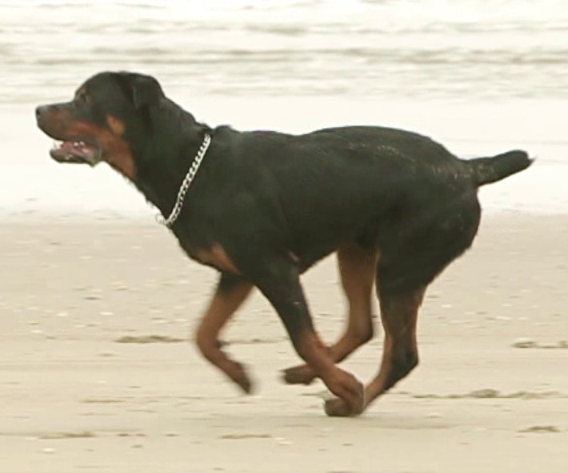
\includegraphics[width=1\linewidth]{input/66}
    \end{subfigure}%
    \begin{subfigure}{0.33\textwidth}
    \centering
        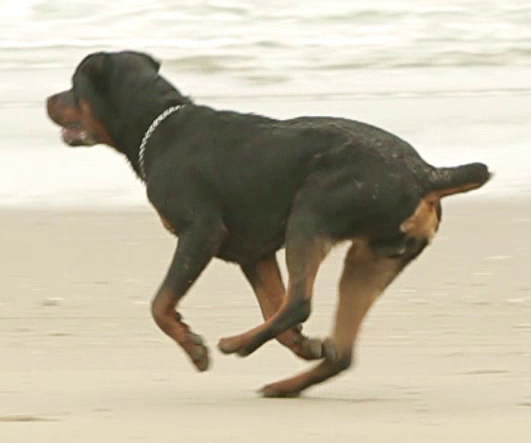
\includegraphics[width=1\linewidth]{input/167}
    \end{subfigure}%
    \begin{subfigure}{0.33\textwidth}
    \centering
        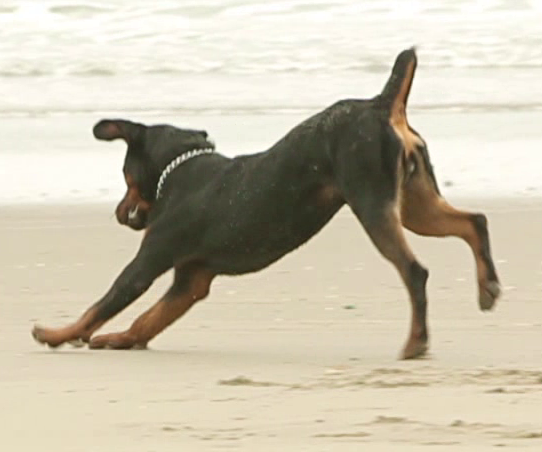
\includegraphics[width=1\linewidth]{input/208}
    \end{subfigure}%
    \caption{An example input video sequence.}
    \label{fig:arap_input}
\end{figure}

    % An example output showing the recovery of a 3D model from an input 2D monocular video is shown in Figure \ref{fig:intro_arap_output}:
    
    % \begin{figure}[H]
    %     \centering
    %     \begin{subfigure}{1\textwidth}
    %     \centering
    %         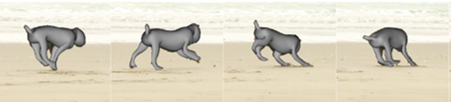
\includegraphics[width=1\linewidth]{input/arapsfm_output}
    %     \end{subfigure}%
    %     \caption{Sample output printed from Deformable Mesh Animation~\cite{arap_stebbing}.}
    %     \label{fig:intro_arap_output}
    % \end{figure}

As elluded to in the previous section, a distinction should be made between two common tracking techniques: (1) discriminative body part recognizers and joint position predictors, and (2) 3D reconstructions via generative model fitting. Discriminative predictors are a popular alternative to full mesh recovery, and have facilitated common use-cases, such as gesture detection or controllerless gameplay. However, to enable animal \emph{shape} recovery, the work in this thesis is closer to approaches that recover full 3D surface models of human subjects. Applications are found in fashion to faciliate online `try-ons' for virtual clothing~\cite{lin2014digital}, in animation and visual effects to generate virtual characters from live actor performances~\cite{laine2017production}, and in healthcare for tracking patients' body weight over time~\cite{velardo2010weight}. 

%It is hypothesized that recovering a full 3D animal reconstruction is necessary to enable the intended diagnostic purposes of this animal work. In particular, returning only joint positions or body parts may be insufficient to estimate animal weight. If this can be realized, identifying behavioural changes from the reconstruction is expected to be a relatively straightforward machine learning problem. 

A typical method for recovering 3D structure from articulated subjects is via a \emph{model fitting} approach, in which a representative 3D morphable model is adapted to recreate the performance of the target. This method involves: (1) designing a suitable 3D morphable model with shape and pose parameterized that represent the target animal species, and (2) designing a machine learning algorithm which operates on an input image or video sequence and outputs per-frame parameters. An example of a template mesh is shown in Figure~\ref{fig:arap_template}.

\begin{figure}[t] % Example image
    \center{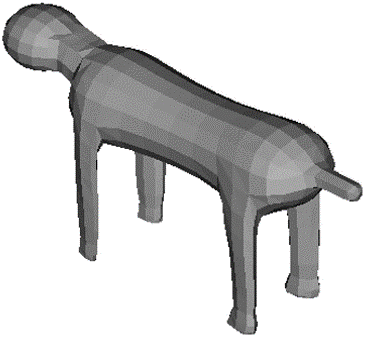
\includegraphics[width=0.2\linewidth]{template_mesh}}
    \caption{An example prior, in this case a template mesh.}
    \label{fig:arap_template}
\end{figure}

Shape attributes capture variation between different members of the target class and therefore remain fixed for a particular individual. For example, shape parameters may be adapted to vary a model's height and weight. However, pose attributes capture limb positions and joint angles, and therefore tend to vary considerably between frames of a capture sequence. Figure~\ref{fig:black_shape} highlights the difference by keeping pose parameters fixed while shape attributes are varied between the three models~\cite{Streuber:SIGGRAPH:2016}.

\begin{figure}[t] % Example image
    \center{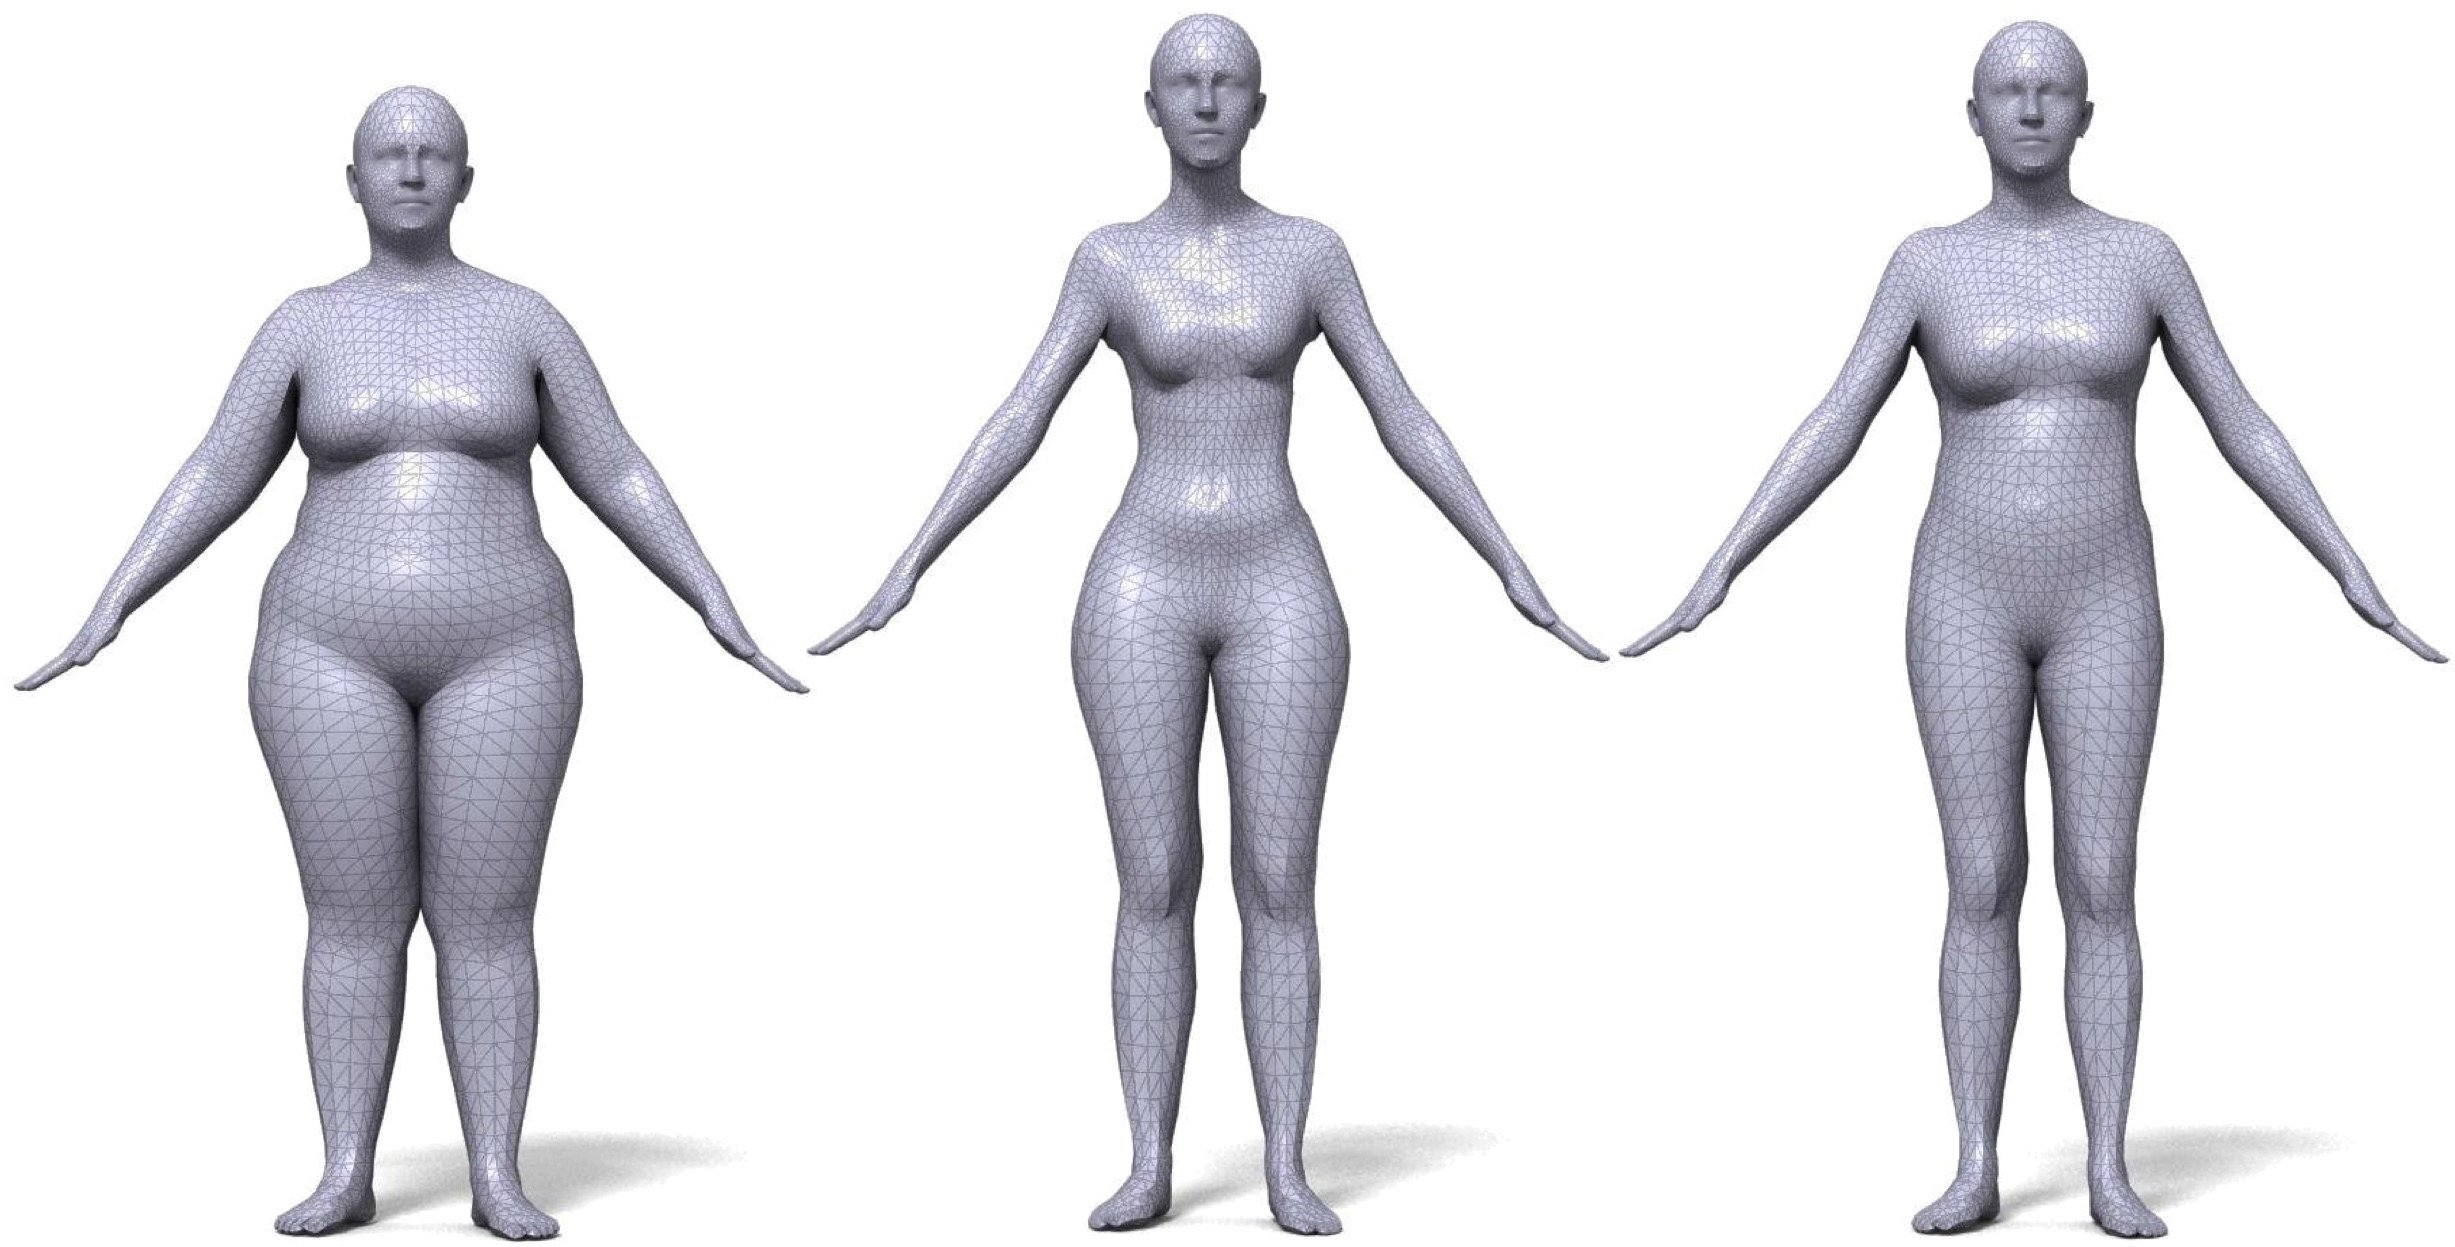
\includegraphics[width=0.9\linewidth]{body_shapes}}
    \caption{Varying human shape parameters while pose remains fixed. Reprinted from~\cite{Streuber:SIGGRAPH:2016}.}
    \label{fig:black_shape}
\end{figure}

Once shape and pose parameters have been derived from a video sequence, they can be applied to the template mesh to generate a digital version of the same activity. If successful, the changing parameters should appear to adapt the template mesh such that it faithfully reproduces the activity of the animal in the input data. 

%In early experimentation, in which tracking targets are restricted to the same species, the template can be chosen to be a close shape fit to the target animal, thereby largely reducing the problem to finding optimal per-frame pose parameters. However, tracking examples are eventually broadened to include a wide range of animal species.

\section{Relation to human reconstruction}
% NEEDS TIDYING
In recent times, 3D human reconstruction has become an established computer vision subfield. It is therefore natural to question to what extent techniques developed for this purpose transfer to the animal case. Some aspects of this are considered:

% Of course, there is some overlap in challenges between animal and human subjects, most notably in the need to reconstruct self-deforming objects which frequently self-occlude. However, additional challenges are posed for animals due to the complex diversity in shape, pose and texture between animal tracking candidates, the limited availability of 3D data for training algorithms and the prevalence of environmental/object occlusion, particularly in internet animal imagery.  However, one advantageous aspect when tracking animals over humans is the simple fact that animals tend not to wear clothing, which in humans causes significant shape and appearance variability.


\subsection{Self-deforming objects.} Animal and human subjects have control over the position of their limbs, for purposes of movement and expression. Capturing these complex motions is of generally important to ensure reconstructions are anatomically plausible. For quadrupedal animals, limb reasoning can be made more difficult due to four legs (rather than two for humans) in rapid motion in a small area. This increases self-occlusion and can make it more challenging to distinguish between left/right and back/front.

\subsection{Variability.}
The variation of shape across and within animal species is considerably greater than in humans and variations in surface texture are considerably larger and more complex than in humans. One advantageous aspect of tracking animals rather than humans is that animals generally do not wear clothing. 

% In one sense, AT is simpler than human tracking as animals generally do not wear clothing. However, variations in surface texture are still considerable between individuals, and the variety of shape across and within species is considerably greater.  If tracking is specialized to a particular species, then shape variation is smaller, but training data is even harder to obtain.

\subsection{Training data.}
For human tracking, hand labelled sequences of 2D segmentations and joint positions have been collected from a wide variety of sources~\cite{andriluka14cvpr,lin2014microsoft,johnson2010clustered}. Of these two classes of labelling, animal {\em segmentation} data is available in datasets such as MSCOCO~\cite{lin2014microsoft}, PASCAL VOC~\cite{everingham2010pascal} and DAVIS~\cite{Perazzi2016}.  However this data is considerably sparser than human data, and must be ``shared'' across species, meaning the number of examples for a given animal shape class is considerably fewer than is available for an equivalent variation in human shape.  While segmentation data can be supplied by non-specialist human labellers, it is more difficult to obtain {\em joint position} data.  Some joints are easy to label, such as ``tip of snout'', but others such as the analogue of ``right elbow'' require training of the operator to correctly identify across species.

Of more concern however, is 3D skeleton data.  For humans, motion capture (mocap) can be used to obtain long sequences of skeleton parameters (joint positions and angles) from a wide variety of motions and activities.
For animal tracking, this is considerably harder: animals behave differently on treadmills than in their quotidian environments, and although some animals such as horses and dogs have been coaxed into motion capture studios~\cite{wilhelm2015furyexplorer}, it remains impractical to consider mocap for a family of tigers at play.

% The previous chapter discussed the primary objective of this work, which is to recover full 3D shape and pose from a live input video sequence exhibiting an animal subject. As explained, the major challenge common to all methods operating on monocular RGB input is to resolve the inherent depth ambiguity associated with recovering a 3D model from 2D input. Competitive methods achieve this by relying on strong motion cues~\cite{kinect_fusion} or (if available) by incorporating strong prior knowledge of the tracking target. Strong shape and pose priors (e.g. body part configuration, acceptable body part lengths, likely joint positions etc.) are available for this problem, so this report will focus on analysing these methods in the literature.

% All solutions face an important design decision, which is to make a distinction between features of an input sequence the system should aim to model and to which it should remain invariant. For example, nearly all human systems aim to model the angle between a tracking target's upper and lower leg region, but nearly all will attempt to remain invariant to skin colour variation between candidates. The next two sections discuss examples of systems in which this decision has been made differently, generally according to the intended real-world application.

% We address this problem using techniques from the recent human body and hand tracking literature, combining machine learning and 3D model fitting.  A discriminative front-end uses a deep hourglass network to identify candidate 2D joint positions. These joint positions are then linked into coherent skeletons by solving an optimal joint assignment problem, and the resulting skeletons create an initial estimate for a generative model-fitting back-end to yield detailed shape and pose for each frame of the video.  

% Although superficially similar to human tracking, animal tracking (AT) has some interesting differences that make it worthy of study:

% \subsubsection*{Variability.}
% In one sense, AT is simpler than human tracking as animals generally do not wear clothing. However, variations in surface texture are still considerable between individuals, and the variety of shape across and within species is considerably greater.  If tracking is specialized to a particular species, then shape variation is smaller, but training data is even harder to obtain.

% \subsubsection*{Training data.}


% \begin{figure}[H] % Example image
%     \center{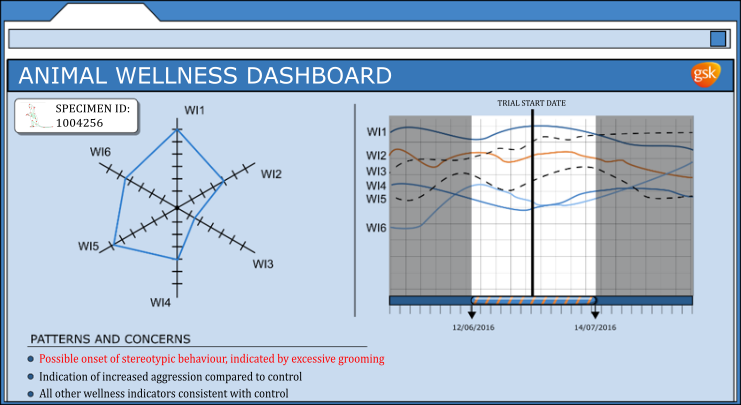
\includegraphics[width=0.95\linewidth]{dash}}
%     \caption{Concept drawing showing an animal health dashboard. Specific wellness markers WI1,...,WI6 have yet to be determined.}
%     \label{fig:wellness_dashboard}
% \end{figure}


%********************************** % Third Section  *************************************
\section{Contributions}  %Section - 1.3 
This thesis tackles key challenges associated with deriving 3D dense reconstructions of animal subjects from monouclar input images and video sequences. \Cref{chap:relwork} contains an in-depth literature review of works focusing on 3D reconstruction of articulated subjects. Specific attention is put towards approaches for designing 3D morphable models, and strategies for predicting the parameters from input data. 

\Cref{chap:cgas} introduces an approach for 3D animal reconstruction and overcomes the limited availability of real world 3D training data for animals by generating synthetic training images. A deep neural network is trained on these images and tested on real world examples to produce estimated joint positions. Importantly, generalizability is ensured by working with silhouette images. The joint predictions are adjusted using a discrete optimization, before a model fitting procedure recovers the full 3D animal model. The method is tested on a range of animal videos and is the first to demonstrate full 3D animal mesh recovery with with no required user intervention. 

\Cref{chap:wldo} describes an end-to-end and real-time neural network which recovers accurate 3D reconstructions for the challenging dog category, trained using weak 2D supervision. The chapter introduces SMBLD, a new 3D deformable template model which includes additional limb scaling parameters and a detailed shape prior learnt during network training. The method is shown to be state-of-the-art on a new StanfordExtra dataset, the largest of its kind for animals, improving over competitive energy minimization techniques even when they are given access to ground truth data. 

\Cref{chap:3dmulti} tackles the problem of recovering 3D reconstructions when given input images exhibiting significant sources of ambiguity, such as environmental occlusion or a partial views of the subject. Rather than attempting to recover a reconstruction uniquely, a multi-hypothesis neural network outputs a set of plausible and varied reconstructions all consistent with the input image. The network is trained according to a best-of-$M$ loss, to which flexibility is added using a novel quantization scheme based on normalizing flows. 

\section{Co-Authored Papers}  %Section - 1.4

This thesis is in part derived from three co-authored publications. \Cref{chap:cgas} contains work from:

\begin{quote}
    \textbf{Benjamin Biggs}, Thomas Roddick, Andrew Fitzgibbon and Roberto Cipolla. \emph{Creatures Great and SMAL: Recovering the Shape and Motion of Animals from Video}. ACCV 2018, Oral Presentation.
\end{quote}

\noindent
\Cref{chap:wldo} contains work from:

\begin{quote}
    \textbf{Benjamin Biggs}, Oliver Boyne, James Charles, Andrew Fitzgibbon and Roberto Cipolla. \emph{Who Left the Dogs Out? 3D Animal Reconstruction with Expectation Maximization In the Loop}. ECCV 2020.
\end{quote}

\noindent
\Cref{chap:3dmulti} contains work from:

\begin{quote}
    \textbf{Benjamin Biggs}, Sebastien Ehrhadt, Hanbyul Joo, Benjamin Graham, Andrea Vedaldi and David Novotny. \emph{3D Multi-bodies: Fitting Sets of Plausible 3D Human Models to Ambiguous Image Data}. NeurIPS 2020, Spotlight Presentation.
\end{quote}
% %!TEX root = ../thesis.tex
%*******************************************************************************
%****************************** Second Chapter *********************************
%*******************************************************************************

\chapter{Related Work}

\ifpdf
    \graphicspath{{Chapter2/Figs/Raster/}{Chapter2/Figs/PDF/}{Chapter2/Figs/}}
\else
    \graphicspath{{Chapter2/Figs/Vector/}{Chapter2/Figs/}}
\fi


\section[Short title]{Reasonably long section title}

% Uncomment this line, when you have siunitx package loaded.
%The SI Units for dynamic viscosity is \si{\newton\second\per\metre\squared}.
I'm going to randomly include a picture Figure~\ref{fig:minion}.


If you have trouble viewing this document contact Krishna at: \href{mailto:kks32@cam.ac.uk}{kks32@cam.ac.uk} or raise an issue at \url{https://github.com/kks32/phd-thesis-template/}


\begin{figure}[htbp!] 
\centering    

\includegraphics[width=1.0\textwidth]{minion}
\caption[Minion]{This is just a long figure caption for the minion in Despicable Me from Pixar}
\label{fig:minion}
\end{figure}


\section*{Enumeration}
Lorem ipsum dolor sit amet, consectetur adipiscing elit. Sed vitae laoreet lectus. Donec lacus quam, malesuada ut erat vel, consectetur eleifend tellus. Aliquam non feugiat lacus. Interdum et malesuada fames ac ante ipsum primis in faucibus. Quisque a dolor sit amet dui malesuada malesuada id ac metus. Phasellus posuere egestas mauris, sed porta arcu vulputate ut. Donec arcu erat, ultrices et nisl ut, ultricies facilisis urna. Quisque iaculis, lorem non maximus pretium, dui eros auctor quam, sed sodales libero felis vel orci. Aliquam neque nunc, elementum id accumsan eu, varius eu enim. Aliquam blandit ante et ligula tempor pharetra. Donec molestie porttitor commodo. Integer rutrum turpis ac erat tristique cursus. Sed venenatis urna vel tempus venenatis. Nam eu rhoncus eros, et condimentum elit. Quisque risus turpis, aliquam eget euismod id, gravida in odio. Nunc elementum nibh risus, ut faucibus mauris molestie eu.
 Vivamus quis nunc nec nisl vulputate fringilla. Duis tempus libero ac justo laoreet tincidunt. Fusce sagittis gravida magna, pharetra venenatis mauris semper at. Nullam eleifend felis a elementum sagittis. In vel turpis eu metus euismod tempus eget sit amet tortor. Donec eu rhoncus libero, quis iaculis lectus. Aliquam erat volutpat. Proin id ullamcorper tortor. Fusce vestibulum a enim non volutpat. Nam ut interdum nulla. Proin lacinia felis malesuada arcu aliquet fringilla. Aliquam condimentum, tellus eget maximus porttitor, quam sem luctus massa, eu fermentum arcu diam ac massa. Praesent ut quam id leo molestie rhoncus. Praesent nec odio eget turpis bibendum eleifend non sit amet mi. Curabitur placerat finibus velit, eu ultricies risus imperdiet ut. Suspendisse lorem orci, luctus porta eros a, commodo maximus nisi.

Nunc et dolor diam. Phasellus eu justo vitae diam vehicula tristique. Vestibulum vulputate cursus turpis nec commodo. Etiam elementum sit amet erat et pellentesque. In eu augue sed tortor mollis tincidunt. Mauris eros dui, sagittis vestibulum vestibulum vitae, molestie a velit. Donec non felis ut velit aliquam convallis sit amet sit amet velit. Aliquam vulputate, elit in lacinia lacinia, odio lacus consectetur quam, sit amet facilisis mi justo id magna. Curabitur aliquet pulvinar eros. Cras metus enim, tristique ut magna a, interdum egestas nibh. Aenean lorem odio, varius a sollicitudin non, cursus a odio. Vestibulum ante ipsum primis in faucibus orci luctus et ultrices posuere cubilia Curae; 
\begin{enumerate}
\item The first topic is dull
\item The second topic is duller
\begin{enumerate}
\item The first subtopic is silly
\item The second subtopic is stupid
\end{enumerate}
\item The third topic is the dullest
\end{enumerate}
Morbi bibendum est aliquam, hendrerit dolor ac, pretium sem. Nunc molestie, dui in euismod finibus, nunc enim viverra enim, eu mattis mi metus id libero. Cras sed accumsan justo, ut volutpat ipsum. Nam faucibus auctor molestie. Morbi sit amet eros a justo pretium aliquet. Maecenas tempor risus sit amet tincidunt tincidunt. Curabitur dapibus gravida gravida. Vivamus porta ullamcorper nisi eu molestie. Ut pretium nisl eu facilisis tempor. Nulla rutrum tincidunt justo, id placerat lacus laoreet et. Sed cursus lobortis vehicula. Donec sed tortor et est cursus pellentesque sit amet sed velit. Proin efficitur posuere felis, porta auctor nunc. Etiam non porta risus. Pellentesque lacinia eros at ante iaculis, sed aliquet ipsum volutpat. Suspendisse potenti.

Ut ultrices lectus sed sagittis varius. Nulla facilisi. Nullam tortor sem, placerat nec condimentum eu, tristique eget ex. Nullam pretium tellus ut nibh accumsan elementum. Aliquam posuere gravida tellus, id imperdiet nulla rutrum imperdiet. Nulla pretium ullamcorper quam, non iaculis orci consectetur eget. Curabitur non laoreet nisl. Maecenas lacinia, lorem vel tincidunt cursus, odio lorem aliquet est, gravida auctor arcu urna id enim. Morbi accumsan bibendum ipsum, ut maximus dui placerat vitae. Nullam pretium ac tortor nec venenatis. Nunc non aliquet neque. 

\section*{Itemize}
\begin{itemize}
\item The first topic is dull
\item The second topic is duller
\begin{itemize}
\item The first subtopic is silly
\item The second subtopic is stupid
\end{itemize}
\item The third topic is the dullest
\end{itemize}

\section*{Description}
\begin{description}
\item[The first topic] is dull
\item[The second topic] is duller
\begin{description}
\item[The first subtopic] is silly
\item[The second subtopic] is stupid
\end{description}
\item[The third topic] is the dullest
\end{description}


\clearpage

\tochide\section{Hidden section}
\textbf{Lorem ipsum dolor sit amet}, \textit{consectetur adipiscing elit}. In magna nisi, aliquam id blandit id, congue ac est. Fusce porta consequat leo. Proin feugiat at felis vel consectetur. Ut tempus ipsum sit amet congue posuere. Nulla varius rutrum quam. Donec sed purus luctus, faucibus velit id, ultrices sapien. Cras diam purus, tincidunt eget tristique ut, egestas quis nulla. Curabitur vel iaculis lectus. Nunc nulla urna, ultrices et eleifend in, accumsan ut erat. In ut ante leo. Aenean a lacinia nisl, sit amet ullamcorper dolor. Maecenas blandit, tortor ut scelerisque congue, velit diam volutpat metus, sed vestibulum eros justo ut nulla. Etiam nec ipsum non enim luctus porta in in massa. Cras arcu urna, malesuada ut tellus ut, pellentesque mollis risus.Morbi vel tortor imperdiet arcu auctor mattis sit amet eu nisi. Nulla gravida urna vel nisl egestas varius. Aliquam posuere ante quis malesuada dignissim. Mauris ultrices tristique eros, a dignissim nisl iaculis nec. Praesent dapibus tincidunt mauris nec tempor. Curabitur et consequat nisi. Quisque viverra egestas risus, ut sodales enim blandit at. Mauris quis odio nulla. Cras euismod turpis magna, in facilisis diam congue non. Mauris faucibus nisl a orci dictum, et tempus mi cursus.

Etiam elementum tristique lacus, sit amet eleifend nibh eleifend sed \footnote{My footnote goes blah blah blah! \dots}. Maecenas dapibu augue ut urna malesuada, non tempor nibh mollis. Donec sed sem sollicitudin, convallis velit aliquam, tincidunt diam. In eu venenatis lorem. Aliquam non augue porttitor tellus faucibus porta et nec ante. Proin sodales, libero vitae commodo sodales, dolor nisi cursus magna, non tincidunt ipsum nibh eget purus. Nam rutrum tincidunt arcu, tincidunt vulputate mi sagittis id. Proin et nisi nec orci tincidunt auctor et porta elit. Praesent eu dolor ac magna cursus euismod. Integer non dictum nunc.


\begin{landscape}

\section*{Subplots}
I can cite Wall-E (see Fig.~\ref{fig:WallE}) and Minions in despicable me (Fig.~\ref{fig:Minnion}) or I can cite the whole figure as Fig.~\ref{fig:animations}


\begin{figure}
  \centering
  \begin{subfigure}[b]{0.3\textwidth}
    
\includegraphics[width=\textwidth]{TomandJerry}
    \caption{Tom and Jerry}
    \label{fig:TomJerry}   
  \end{subfigure}             
  \begin{subfigure}[b]{0.3\textwidth}
    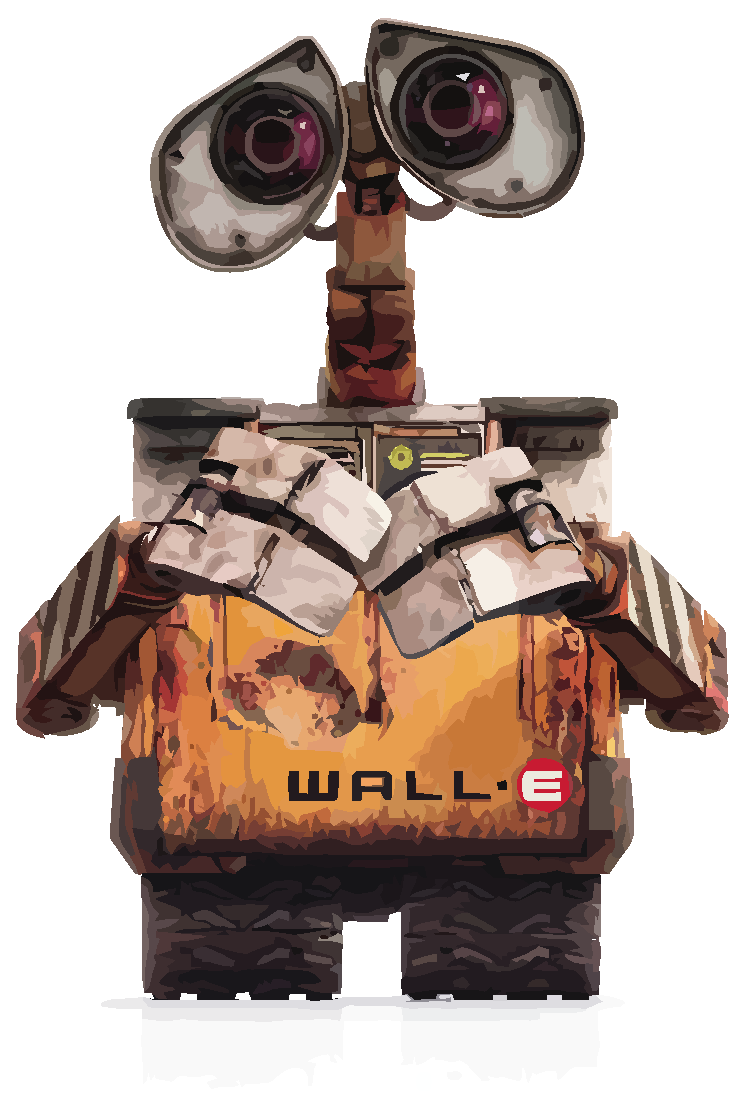
\includegraphics[width=\textwidth]{WallE}
    \caption{Wall-E}
    \label{fig:WallE}
  \end{subfigure}             
  \begin{subfigure}[b]{0.3\textwidth}
    
\includegraphics[width=\textwidth]{minion}
    \caption{Minions}
    \label{fig:Minnion}
  \end{subfigure}
  \caption{Best Animations}
  \label{fig:animations}
\end{figure}


\end{landscape}

%!TEX root = ../thesis.tex
%*******************************************************************************
%****************************** Third Chapter **********************************
%*******************************************************************************
\chapter{Learning from Synthetic Data}

% **************************** Define Graphics Path **************************
\ifpdf
    \graphicspath{{Chapter3/Figs/Raster/}{Chapter3/Figs/PDF/}{Chapter3/Figs/}}
\else
    \graphicspath{{Chapter3/Figs/Vector/}{Chapter3/Figs/}}
\fi

\section{Introduction}
And now I begin my third chapter here \dots

\begin{enumerate}
  \item We want precise shape reconstructions in real-time
  \item Refer back to SMAL-ST, requires 3D synthetic training data from video
  \item A whole chapter on 'training in-the-loop' methods
  \item Talk about expectation maximization, SMBLD, EM-in-the-loop
  \item Optional: Talk about how this can be extended to a multi-view GSK setup, similar to MeshRCNN
\end{enumerate}

\begin{abstract}
  We present a system to recover the 3D shape and motion of a wide variety of quadrupeds from video.  The system comprises a machine learning front-end which predicts candidate 2D joint positions, a discrete optimization which finds kinematically plausible joint correspondences, 
  and an energy minimization stage which fits a detailed 3D model to the image. In order to overcome the limited availability of motion capture training data from animals, and the difficulty of generating realistic synthetic training images, the system is designed to work on silhouette data.  The joint candidate predictor is trained on synthetically generated silhouette images, and at test time, deep learning methods or standard video segmentation tools are used to extract silhouettes from real data. The system is tested on animal videos from several species, and shows accurate reconstructions of 3D shape and pose.
  \end{abstract}
  %===========================================================
  \section{Introduction}
  
  Animal welfare is an important concern for business and society, with an estimated 70 billion animals currently living under human care~\cite{FAOSTAT}. Monitoring and assessment of animal health can be assisted by obtaining accurate measurements of an individual's shape, volume and movement. These measurements should be taken without interfering with the animal's normal activity, and are needed around the clock, under a variety of lighting and weather conditions, perhaps at long range (e.g.\ in farm fields or wildlife parks). Therefore a very wide range of cameras and imaging modalities must be handled. For small animals in captivity, a depth camera might be possible, but techniques which can operate solely from intensity data will have a much wider range of applicability.
  
  We address this problem using techniques from the recent human body and hand tracking literature, combining machine learning and 3D model fitting.  A discriminative front-end uses a deep hourglass network to identify candidate 2D joint positions. These joint positions are then linked into coherent skeletons by solving an optimal joint assignment problem, and the resulting skeletons create an initial estimate for a generative model-fitting back-end to yield detailed shape and pose for each frame of the video.  
  
  \def\bb{\rule{2in}{0pt}\rule{0pt}{1in}}
  
  \begin{figure}[t]
  \def\p#1#2{\parbox{0.32\linewidth}{
  \labelledpic{\includegraphics[trim={4cm 7cm 4cm 7cm},clip,width=\linewidth]{sys_overview_pred_2/#2.jpg}}
  {\scriptsize #1}}}
  \def\ps#1#2{\parbox{0.32\linewidth}{
  \labelledpic{\includegraphics[trim={0cm 2cm 0cm 2cm},clip,width=\linewidth]{sys_overview_pred_2/#2.jpg}}
  {\scriptsize #1}}}
  \p a{rgb}             \p b{target}         \p c{heatmap}
  \p d{skeleton_sil}    \p e{00048_overlay}  \ps f{00048_alternative}
  \caption{{\bf System overview}: input video (a) is automatically processed using DeepLabv3+~\cite{deeplabv3plus} to produce silhouettes (b), from which 2D joint predictions are regressed in the form of heatmaps (c).  Optimal joint assignment (OJA) finds kinematically coherent 2D-to-3D correspondences~(d), 
  which initialize a 3D shape model, optimized to match the silhouette~(e). 
  Alternative view shown in (f).
  }
  \label{fig:overview}
  \end{figure}
  
  Although superficially similar to human tracking, animal tracking (AT) has some interesting differences that make it worthy of study:
  
  \subsubsection*{Variability.}
  In one sense, AT is simpler than human tracking as animals generally do not wear clothing. However, variations in surface texture are still considerable between individuals, and the variety of shape across and within species is considerably greater.  If tracking is specialized to a particular species, then shape variation is smaller, but training data is even harder to obtain.
  
  \subsubsection*{Training data.}
  For human tracking, hand labelled sequences of 2D segmentations and joint positions have been collected from a wide variety of sources~\cite{andriluka14cvpr,mscoco,johnson2010clustered}. Of these two classes of labelling, animal {\em segmentation} data is available in datasets such as MSCOCO~\cite{mscoco}, PASCAL VOC~\cite{pascal-voc-2012} and DAVIS~\cite{Perazzi2016}.  However this data is considerably sparser than human data, and must be ``shared'' across species, meaning the number of examples for a given animal shape class is considerably fewer than is available for an equivalent variation in human shape.  While segmentation data can be supplied by non-specialist human labellers, it is more difficult to obtain {\em joint position} data.  Some joints are easy to label, such as ``tip of snout'', but others such as the analogue of ``right elbow'' require training of the operator to correctly identify across species.
  
  Of more concern however, is 3D skeleton data.  For humans, motion capture (mocap) can be used to obtain long sequences of skeleton parameters (joint positions and angles) from a wide variety of motions and activities.
  For animal tracking, this is considerably harder: animals behave differently on treadmills than in their quotidian environments, and although some animals such as horses and dogs have been coaxed into motion capture studios~\cite{wilhelm2015furyexplorer}, it remains impractical to consider mocap for a family of tigers at play.
  
  These concerns are of course alleviated if we have access to synthetic training data.  Here, humans and animals share an advantage in the availability of parameterized 3D models of shape and pose.  The recent publication of the Skinned Multi-Animal Linear (SMAL) model~\cite{zuffi2017menagerie} can generate a wide range of quadruped species, although without surface texture maps.  However, as with humans, it remains difficult to generate RGB images which are sufficiently realistic to train modern machine learning models.  In the case of humans, this has been overcome by generating depth maps, but this then requires a depth camera at test time~\cite{shotton-kinect}. The alternative, used in this work, is to generate 2D silhouette images so that machine learning will predict joint heatmaps from silhouettes only.
  
  Taking into account the above constraints, this work applies a novel strategy to animal tracking, which assumes a machine-learning approach to extraction of animal silhouettes from video, and then fits a parameterized 3D model to silhouette sequences.  We make the following contributions:
  \begin{itemize}
  \item A machine-learned mapping from silhouette data of a large class of quadru\-peds to generic 2D joint positions.
  \item A novel optimal joint assigment (OJA) algorithm extending the bipartite matching of Cao {\em et al.}~\cite{cao2017realtime} in two ways, one which can be cast as a quadratic program (QP), and an extension optimized using a genetic algorithm (GA).
  \item A procedure for optimization of a 3D deformable model to fit 2D silhouette data and 2D joint positions, while encouraging temporally coherent outputs.
  \item We introduce a new benchmark animal dataset of joint annotations (BADJA) which contains sparse keypoint labels and silhouette segmentations for eleven animal video sequences. 
  Previous work in 3D animal reconstruction has relied on bespoke hand-clicked keypoints~\cite{zuffi2017menagerie,zuffi_lions} and little quantitative evaluation of performance could be given.
  The sequences exhibit a range of animals, are selected to capture a variety of animal movement and include some challenging visual scenarios such as occlusion and motion blur.
  \end{itemize}
  The system is outlined in \figref{overview}.  The remainder of the paper describes related literature before a detailed description of system components.  Joint accuracy results at multiple stages of the pipeline are reported on the new BADJA dataset, which contains ground truths for real animal subjects. We also conduct experiments on synthetic animal videos to produce joint accuracy statistics and full 3D mesh comparisons. A qualitative comparison is given to recent work~\cite{zuffi2017menagerie} on the related single-frame 3D shape and pose recovery problem. The paper concludes with an assessment of strengths and limitations of the work.
  \newpage
  \section{Related work}
  3D animal tracking is relatively new to the computer vision literature, but animal breed identification is a well studied problem~\cite{imagenet_cvpr09}. Video tracking benchmarks often use animal sequences~\cite{DAVIS2017-1st,DAVIS2017-2nd}, although the tracking output is typically limited to 2D affine transformations rather than the detailed 3D mesh that we propose.  Although we believe our work is the first to demonstrate dense 3D tracking of animals in video without the need for user-provided keypoints, we do build on related work across computer vision:
  
  \subsubsection*{Morphable shape models.}
  Cashman and Fitzgibbon~\cite{cashman2013shape} obtained one of the first 3D morphable animal models, but their work was limited to small classes of objects (e.g. dolphins, pigeons), and did not incorporate a skeleton.  Their work also showed the use of the 2D silhouette for fitting, which is key to our method. 
  Reinert {\em et al.} \cite{reinert2016animated} meanwhile construct 3D meshes by fitting generalized cylinders to hand-drawn skeletons.
  Combined skeletal and morphable models were used by Khamis {\em et al.}~\cite{hand-shape} for modelling the human hand, and Loper {\em et al.}~\cite{loper2015smpl} in the SMPL model which has been extensively used for human tracking. 
  
  The SMPL model was extended to animals by Zuffi {\em et al.}~\cite{zuffi2017menagerie}, where the lack of motion capture data for animal subjects is cleverly overcome by building the model from $41$ 3D scans of toy figurines from five quadruped families in arbitrary poses. Their paper demonstrates single-frame fits of their model to real-world animal data, showing that despite the model being built from ``artists' impressions'' it remains an accurate model of real animals. This is borne out further by our work.  Their paper did however depend on per-frame human annotated keypoint labels, which would be costly and challenging to obtain for large video sequences. This work was recently extended~\cite{zuffi_lions} with a refinement step that optimizes over model vertex positions. This can be considered independent to the initial SMAL model fit and would be trivial to add to our method.
  
  \subsubsection*{Shape from silhouette.} Silhouette images have been shown to contain sufficient shape information to enable their use in many 3D recovery pipelines. Chen {\em et al.}~\cite{chen2010inferring} demonstrate single-view shape reconstruction from such input for general object classes, by building a shape space model from 3D samples. More related to our work, Favreau {\em et al.}~\cite{favreau2004animal} apply PCA to silhouette images to extract animal gaits from video sequences. The task of predicting silhouette images from 2D input has been effectively used as a proxy for regressing 3D model parameters for humans~\cite{indirect2017,hmrKanazawa17} and other 3D objects~\cite{wiles2017silnet}.
  
  \subsubsection*{Joint position prediction.} There is an extensive body of prior work related to joint position prediction for human subjects. Earlier work used graphical approaches such as pictorial structure models~\cite{andriluka2010monocular,pishchulin2013poselet,johnson2010clustered}, which have since been replaced with deep learning-based methods~\cite{cao2017realtime,bulat2016human}. Few works predict animal joint positions directly owing to the lack of annotated data, although Mathis {\em et al.}~\cite{mathis2018deeplabcut} demonstrate the effectiveness of human pose estimation architectures for restricted animal domains. Our method instead trains on silhouette input, allowing the use of synthetic training imagery. The related task of animal part segmentation~\cite{wang2015joint,wang2015semantic} has seen some progress due to general object part datasets~\cite{chen_cvpr14,zhou2017scene}.
  
  \subsection{Preliminaries}
  \def\R#1{{\mathbb{R}^{#1}}}
  \def\RR#1#2{{\mathbb{R}^{#1 \times #2}}}
  \def\posn{\phi}
  \def\pose{\theta}
  \def\npose{P}
  \def\shape{\beta}
  \def\nshape{B}
  \def\verts{\nu}
  \def\nverts{V}
  \def\jointselect{\mathtt{K}}
  \def\njoints{J}
  We are given a deformable 3D model such as SMAL~\cite{zuffi2017menagerie} which parametrizes a 3D mesh as a function of {\em pose} parameters~$\pose \in \R\npose$ (e.g.\ joint angles) and {\em shape} parameters~$\shape \in \R\nshape$. 
  In detail, a 3D mesh is an array of vertices $\verts \in \RR 3\nverts$ (the vertices are columns of a $3 \times \nverts$ matrix) and a set of triangles represented as integer triples $(i,j,k)$, which are indices into the vertex array.
  A deformable model such as SMPL or SMAL may be viewed as supplying a set of triangles, and a function
  \begin{equation}
  \verts(\pose, \shape) : \R \npose \times \R \nshape \mapsto \RR 3 \nverts
  \end{equation}
  which generates the 3D model for a given pose and shape.
  The mesh topology (i.e.~the triangle vertex indices) is provided by the deformable model, and is the same for all shapes and poses we consider, so in the sequel we shall consider a mesh to be defined only by the 3D positions of its vertices.
  
  In any given image, the model's 3D {\em position} (i.e.\ translation and orientation) is also unknown, and will be represented by a parametrization $\posn$ which may be for example translation as a 3-vector and rotation as a unit quaternion. Application of such a transformation to a $3\times\nverts$ matrix will be denoted by $*$, so that 
  \begin{equation}
  \posn * \verts(\pose, \shape)
  \end{equation}
  represents a 3D model of given pose and shape transformed to its 3D position.
  
  \def\proj{\pi}
  We will also have occasion to talk about model {\em joints}.  These appear naturally in models with an explicit skeleton, but more generally they can be defined as some function mapping from the model parameters to an array of 3D points analogous to the vertex transformation above.  We consider the joints to be defined by post-multiplying by a $\nverts \times \njoints$ matrix $\jointselect$.  The $j^{\text{th}}$ column of~$\jointselect$ defines the 3D position of joint~$j$ as a linear combination of the vertices (this is quite general, as $\verts$ may include vertices not mentioned in the triangulation).  A general camera model is described by a function $\proj: \R 3 \mapsto \R 2$.  This function incorporates details of the camera intrinsics such as focal length, which are assumed known.  
  Thus 
  \begin{equation}
  \kappa(\posn, \pose, \shape) := \proj(\posn * \verts(\pose, \shape) \jointselect)
  \end{equation}
  is the $2\times \njoints$ matrix whose columns are 2D joint locations corresponding to a 3D model specified by (position, pose, shape) parameters $(\posn, \pose, \shape)$.
  
  The model is also assumed to be supplied with a rendering function $R$ which takes a vertex array in camera coordinates, and generates a 2D binary image of the model silhouette.  That is,
  \begin{equation}
  R\bigl(\posn * \verts(\pose, \shape)\bigr) \in \mathbb{B}^{W\times H}
  \end{equation}
  for an image resolution of $W \times H$.  We use the differentiable renderer of Loper {\em et al.}~\cite{loper2014opendr} to allow derivatives to be propagated through $R$.  
  \newpage
  \section{Method}
  \def\seq#1#2#3#4{\left[{#1_{#2}}\right]_{#2=#3}^{#4}}
  The test-time problem to be solved is to take a sequence of input images
  $
  \mathcal I = \seq I t1T
  $
  which are segmented to the silhouette of a single animal (i.e.~a video with multiple animals is segmented multiple times), producing a sequence of binary silhouette images 
  $
  \mathcal S = \seq S t1T.
  $
  
  The computational task is to output for each image the shape,  pose, and position parameters describing the animal's motion.
  
  As outlined above, the method has three parts.  
  (1.) The discriminative front-end extracts silhouettes from video, and then uses the silhouettes to predict 2D joint positions, with multiple candidates per joint. 
  (2.) Optimal joint assignment (OJA) corrects confused or missing skeletal predictions by finding an optimal assignment of joints from a set of network-predicted proposals. Finally, (3.) a generative deformable 3D model is fitted to the silhouettes and joint candidates as an energy minimization process.
  
  \subsection{Prediction of 2D joint locations using multimodal heatmaps}
  The goal of the first stage is to take, for each video frame, a $W\times H$ binary image representing the segmented animal, and to output a $W \times H \times \njoints$ tensor of heatmaps. The network architecture is standard: a stacked hourglass network~\cite{newell2016stacked} using synthetically generated training data, but the training procedure is augmented using ``multi-modal'' heatmaps. 
  
  For standard unimodal heatmaps, training data comprises $(S, \kappa)$ pairs, that is pairs of binary silhouette images, and the corresponding 2D joint locations as a $2\times J$ matrix.  To generate each image, a random shape vector $\shape$, pose parameters $\pose$ and camera position $\posn$ are drawn, and used to render a silhouette $R\bigl(\posn * \verts(\pose, \shape)\bigr)$ and 2D joint locations $\kappa(\posn,\pose,\shape)$, which are encoded into a $W \times H \times \njoints$ tensor of heatmaps, blurring with a Gaussian kernel of radius $\sigma$. 
  
  % bjb_insert
  The random camera positions are generated as follows: the orientation of the camera relative to the animal is uniform in the range $[0, 2\pi]$, the distance from the animal is uniform in the range 1 to 20 meters and the camera height is in the range $[0,\frac{\pi}{2}]$. This smaller range is chosen to restrict unusual camera elevation. Finally, the camera ``look" vector is towards a point uniformly in a 1m cube around the animal's center, and the ``up" vector is Gaussian around the model Y axis.  
  
  This training process generalizes well from synthetic to real images due to the use of the silhouette, but the lack of interior contours in silhouette input data often results in confusion between joint ``aliases'': left and right or front and back legs.  When these predictions are wrong and of high confidence, little probability mass is assigned to the area around the correct leg, meaning no available proposal is present after non-maximal suppression.
  
  We overcome this by explicitly training the network to assign some probability mass to the ``aliased'' joints. For each joint, we define a list of potential aliases as weights $\lambda_{j,j'}$ and linearly blend the unimodal heatmaps $G$ to give the final training heatmap $H$:
  \begin{equation}
      H_{j}(p) = \sum_{j'} \lambda_{j,j'} G(p; \kappa_{j'}, \sigma)
  \end{equation}
  For non-aliased joints $j$ (all but the legs), we simply set $\lambda_{j,j} = 1$ and $\lambda_{j,j'} = 0$, yielding the unimodal maps, and for legs, we use 0.75 for the joint, and 0.25 for the alias.  We found this ratio sufficient to ensure opposite legs have enough probability mass to pass through a modest non-maximal suppression threshold without overly biasing the skeleton with maximal predicted confidence. An example of a heatmap predicted by a network trained on multimodal training samples is illustrated in \figref{single_multi}. 
  
  \begin{figure}[t]
  \begin{floatrow}
  \ffigbox{%%%%%%%%%%%%
  \centering
  \begin{tabular}{c}
  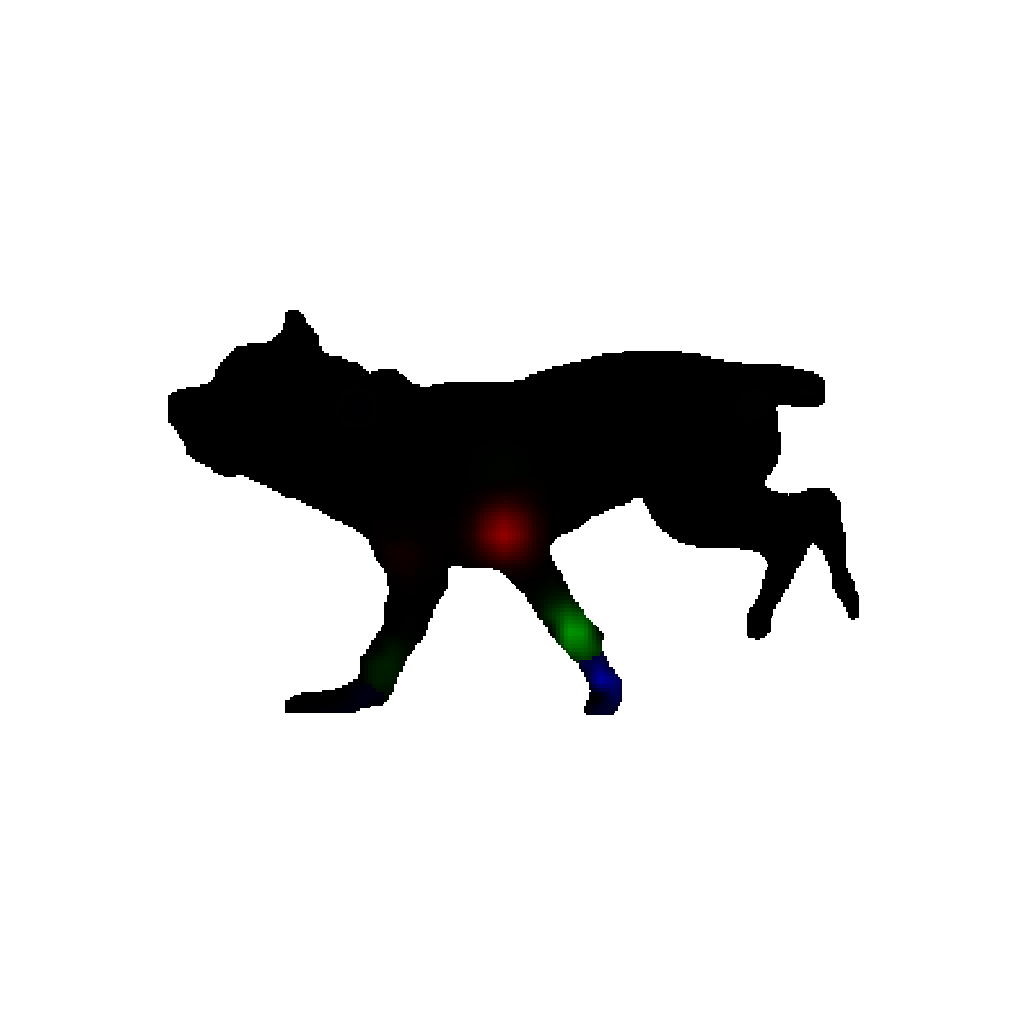
\includegraphics[trim={4cm 10cm 4cm 10cm},clip,width=0.6\linewidth]{single_vs_multi_new/left_heatmap_single.png}\\
  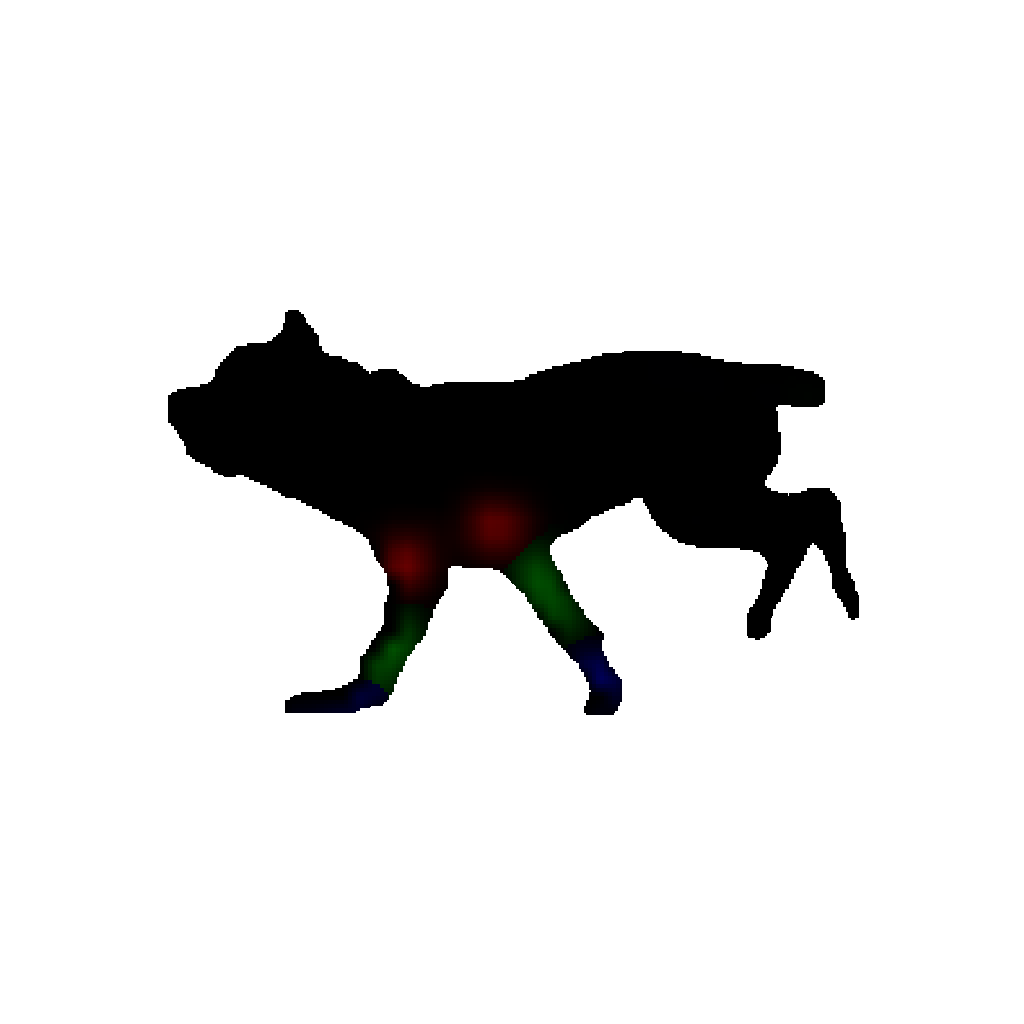
\includegraphics[trim={4cm 10cm 4cm 10cm},clip,width=0.6\linewidth]{single_vs_multi_new/left_heatmap_multi.png}
  \end{tabular}
  }{
  \caption{Example predictions from a network trained on unimodal (top) and multi-modal (bottom) ground-truth  for front-left leg joints.}
  \label{fig:single_multi}
  }
  \ffigbox{
  \centering
  \def\lp#1#2{\labelledpic{\includegraphics[height=19mm]{#2}}{#1}}
  \begin{tabular}{cc}
  \lp a{skeletons_new/skeleton_rgb_dog_cropped.jpg}&
  \lp b{skeletons_new/skeleton_rgb_impala_cropped.jpg}\\
  \lp c{skeletons_new/skeleton_rgb_rhino_cropped.jpg}&
  \lp d{skeletons_new/skeleton_rgb_horsejump-high_cropped.jpg}
  \end{tabular}
  }{
  \caption{Example outputs from the joint prediction network, with maximum likelihood predictions linked into skeleton.}
  \label{fig:exp-network}
  }
  \end{floatrow}
  \end{figure}
  
  \subsection{Optimal joint assignment (OJA)}
  \label{sec:qp}
  Since heatmaps generated by the joint predictor are multi-modal, the non-maximum suppression procedure yields multiple possible locations for each joint. We represent the set of joint proposals $X = \{x_{jp}\}$, where $x_{jp}$ indicates the 2D position of proposal $p \in \{1,...,N_j\}$ associated with joint $j \in J$.
  Before applying the optimizer, we must select a subset of proposals $X^* \subseteq X$ which form a complete skeleton, i.e. precisely one proposal is selected for every joint. In this section we consider how to choose the optimal subset by formulating the problem as an extended optimal assignment problem.
  
  \def\bvec#1{\bar{#1}}
  \def\LL#1{L_{\text{#1}}}
  In order to select a complete skeleton proposal from the set of joint proposals $\{x_{jp}\}$, we introduce a binary indicator vector $\bvec a_j = \{a_{jp}\} \in \{0, 1\}^{N_j+1}$, where $a_{jp} = 1$ indicates that the $p^\text{th}$ proposal for joint $j$ is a correct assignment, and the $p = N_j+1$ position corresponds to a {\em null proposal}, indicating that joint $j$ has no match in this image.
  The null proposals are handled as described in each of the energy terms below.
  Let $A$ be the jagged array $[\bvec a_j]_{j=1}^J$ containing all assignment variables (for the current frame), and let $X^* = X(A)$ denote the subset of points selected by the binary array $A$.   
  Optimal assignment minimizes the function
  \begin{equation}
  L(A) = \LL{prior}(A) + \LL{conf}(A) + \LL{temp}(A) + \LL{cov-sil}(A) + \LL{cov-bone}(A)
  \end{equation}
  which balances agreement of the joint configuration with a learned {\em prior}, the network-supplied {\em confidences}, {\em temporal} coherence, and {\em coverage} terms which encourage the  model to correctly project over the silhouette.   Without the coverage terms, this can be optimized as a quadratic program, but we obtain better results by using the coverage terms, and using a genetic algorithm.  In addition, the parameters $A$ must satisfy the $J$ constraints $\sum_{p=1}^{N_j+1} a_{jp} = 1$, that exactly one joint proposal (or the null proposal) must be selected for each joint.
  
  \def\lterm#1{\subsubsection{$\LL{#1}$:}}
  
  \lterm{prior} We begin by defining the prior probability of a particular skeletal configuration as a multivariate Gaussian distribution over selected joint positions.
  
  The mean $\mu \in \R{2J}$ and covariance $\Sigma \in \R{2J\times 2J}$ terms are obtained from the training examples generated as above. The objective of OJA is to select a configuration $X^*$ which maximizes the prior, which is equivalent to minimizing the Mahalanobis distance
  $(x^*-\mu)^T\Sigma^{-1}(x^*-\mu)$, which is given by the summation
  \begin{equation}
  \LL{prior}(A) = \sum_j^J\sum_p^{N_j}\sum_k^J\sum_q^{N_k}a_{jp}a_{kq}(x_{jp} - \mu_j)\Sigma_{jk}^{-1}(x_{kq}-\mu_k)
  \end{equation}
  This is a quadratic function of $A$, so $\LL{prior}(A) = \text{vec}(A)^\top Q \text{vec}(A)$ for a fixed matrix $Q$, and can be formulated as a quadratic program (QP).  Null proposals are simply excluded from the sum, equivalent to marginalizing over their position. 
  
  \lterm{conf}
  The next energy term comes from the output of the joint prediction network, which provides a confidence score $y_{jp}$ associated with each joint proposal~$x_{jp}$.  Then $\LL{conf}(A) = \sum_j\sum_p -\lambda\log(y_{jp}) a_{jp}$ is a linear function of $A$, 
  and $\lambda_{\text{conf}}$ is a tunable parameter to control the relative contribution of the network confidences compared with that of the skeleton prior.
  Null proposals pay a fixed cost $\lambda_{null}$, effectively acting as a threshold whereby the null proposal will be selected if no other proposal is of sufficient likelihood. 
  
  \lterm{temp}
  A common failure case of the joint prediction network is in situations where a joint position is highly ambiguous, for example between the left and right legs. In such cases, the algorithm will commonly alternate between two equally likely predictions. This leads to large displacements in joint positions between consecutive frames which are difficult for the later model fitting stage to recover from. This can be addressed by introducing a temporal term into the OJA. We impose a prior on the distance moved by each joint between frame $t_0$ and $t_1$, which is given by a normal distribution with zero mean and variance $\sigma^{2} =e^{\tau|t_1 - t_0 - 1|}$. 
  The parameter $\tau$ controls the strength of the interaction between distant frames. This results in an additional quadratic term in our objective function, which has the form $L_{temp} = a^\top T^{(t_0, t_1)} a$ for matrix $T^{(t_0, t_1)}$ given by 
  \begin{equation}
  \left[T^{(t_0, t_1)}\right]_{jp, kq} = \begin{cases}
  e^{-\alpha|t_1 - t_0 - 1|}||x^{(t_0)}_{jp} - x^{(t_1)}_{kq}||^2 & \text{if } j=k\\
  0 & \text{otherwise}
  \end{cases}
  \end{equation}
  
  \subsubsection*{QP solution.}
  Thus far, all terms in $L(A)$ are quadratic or linear.
  To optimize over an entire sequence of frames, we construct the block diagonal matrix $\hat{Q}$ whose diagonal elements are the prior matrices $Q^{(t)}$ and the block symmetric matrix $\hat{T}$ whose off-diagonal elements are the temporal matrices $T^{(t_0, t_1)}$. The solution vector for the sequence $\hat{A}$ is constructed by stacking the corresponding vectors for each frame. The quadratic program is specified using the open source CVXPY library \cite{diamond2016cvxpy} and solved using the ``\emph{Suggest-and-Improve}'' framework proposed by Park and Boyd \cite{park2017general}. It is initialized by choosing the proposal with the highest confidence for each joint. Appropriate values for the free parameters $\lambda_{\text{conf}, \text{temp}}$ and $\alpha$ were chosen empirically via grid search. 
  
  \lterm{cov-\{sil,bone\}}
  The above quadratic formulation is sufficient to correct many errors in the raw output (which we later demonstrate in the experimental section), but suffers from an `overcounting' problem, in which leg joint predictions both cover the same silhouette leg region, leaving another leg empty. We therefore extend the definition of $L(A)$ to include two additional terms. 
  
  \def\silhouette{S}
  
  \lterm{cov-sil} penalizes large silhouette areas with no nearby selected joint. This term requires a precomputed set of silhouette sample points $Z \subseteq \mathbb{R}^2$, which we aim to ``cover'' as best as possible with the set of selected joints. Intuitively, the silhouette is considered well-covered if all sample points are close to \emph{some} selected joint proposal. The set $Z$ is generated from the medial axis transform (MAT)\cite{blum1967transformation} of the silhouette, $Z^{t} = \text{MAT}(\silhouette^{t})$
  with a cubed loss strongly penalizing projection outside the silhouette:
  \begin{equation}
  \LL{cov-sil}(A^{t};X^{t},Z^{t}) = \sum_{i}\min_{j}\|Z_{i}^{t} - \hat{X}_{j}^{t}\|^3
  \end{equation}
  
  \begin{figure}[t!]
  \begin{floatrow}
  \ffigbox{%%%%%%%%%%%%
  \def\bb{\rule{2in}{0pt}\rule{0pt}{1in}}
  \def\bjb{\rule{0.5in}{0pt}\rule{0pt}{0.25in}}
  
  \begin{center}
  \scalebox{-1}[1]{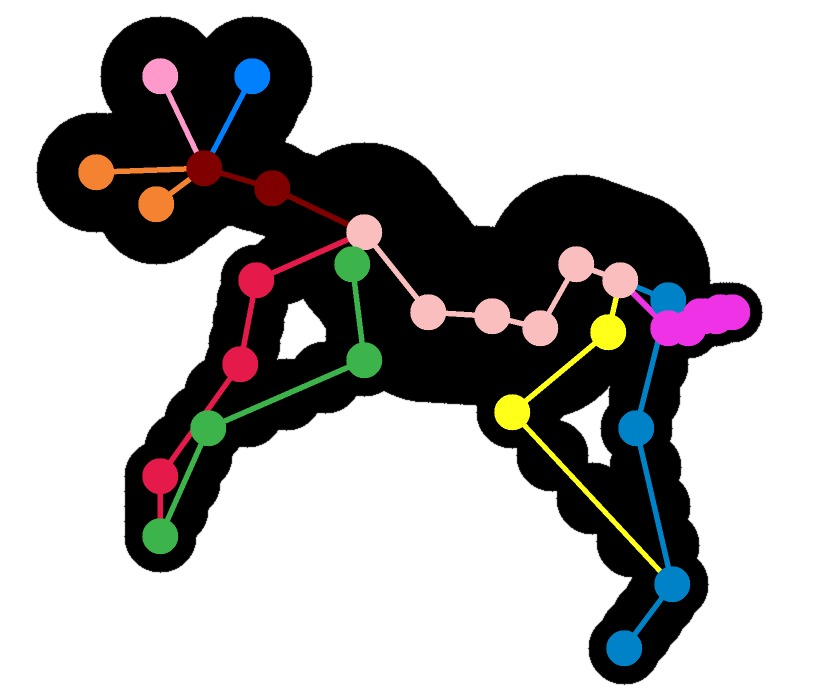
\includegraphics[width=0.49\linewidth]{sil_coverage_new/approx_render_cov_cropped.jpg}}
  \scalebox{-1}[1]{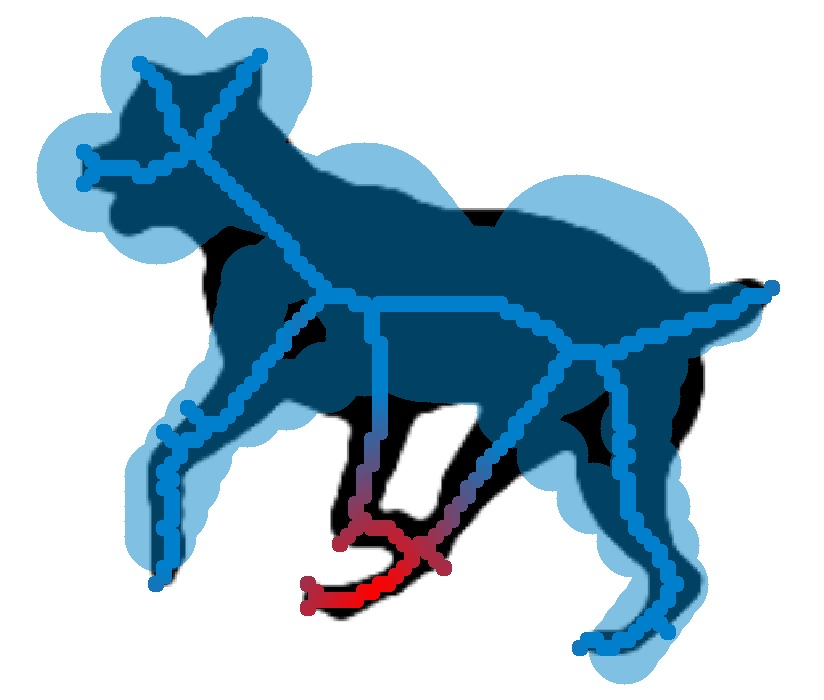
\includegraphics[width=0.49\linewidth]{sil_coverage_new/med_axis_overlay_error_cropped.jpg}}
  % predictions taken from rs_dog frame 0100
  \end{center}
  }
  {\caption{Silhouette coverage loss. The error (shown in red) is the the distance between the median axis transform (right) and the nearest point on an approximate rendering (left).}
  \label{fig:example_errors}}
  \ffigbox{ 
      \raisebox{1 em}{
      \centering
      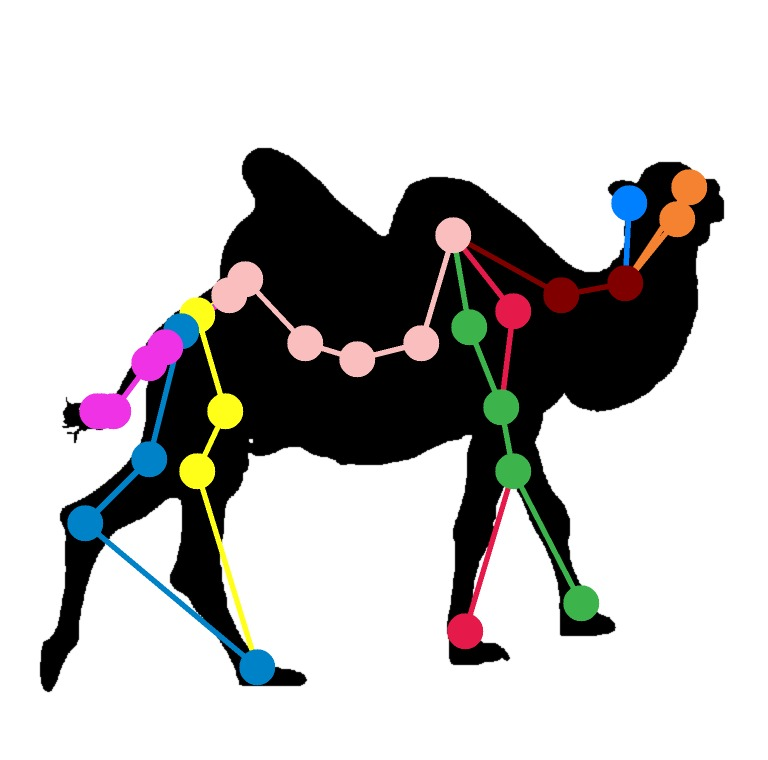
\includegraphics[trim={0cm 0cm 0cm 0cm}, clip,width=0.45\linewidth]{bone_coverage/skeleton_sil_cropped.jpg}
      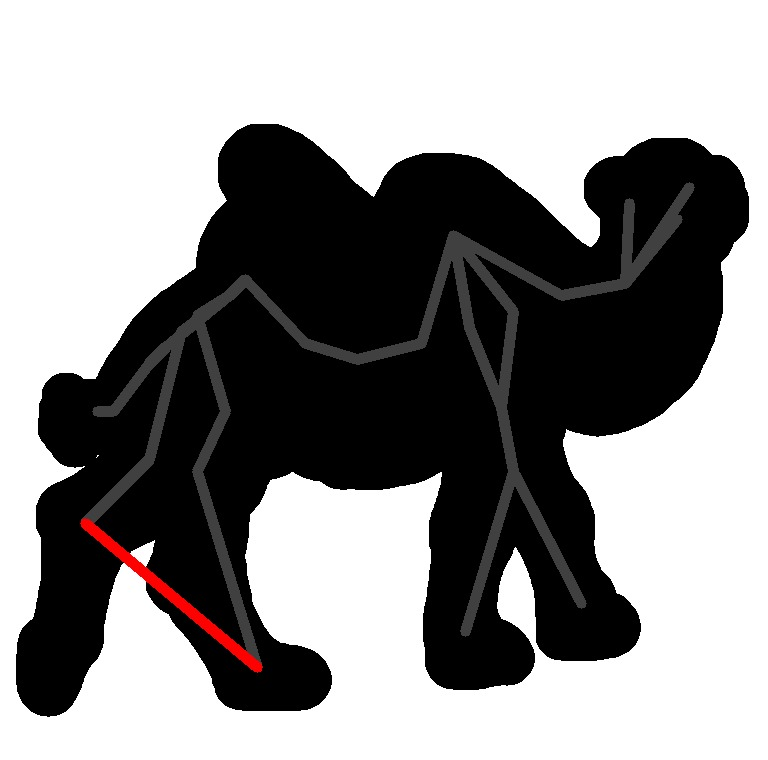
\includegraphics[trim={0cm 0cm 0cm 0cm},clip,width=0.45\linewidth]{bone_coverage/bone_error_overlay_cropped.jpg}
      }
  }
  {\caption{Bone coverage loss. One of the back-right leg joints is incorrectly assigned (left), leading to a large penalty since the lower leg bone crosses outside the dilated silhouette (right).}
  \label{fig:cov-bone}
  % camel 0020}
  }
  \end{floatrow}
  \end{figure}
  
  \lterm{cov-bone} is used to prevent bones crossing the background. The joint hierarchy is stored in a kinematic tree structure $K = \{\{j,k\} \text{ if joints } j, k \text{ are connected by a bone}\}$.
  \begin{equation}
  \LL{cov-bone}(A^{t};X^{t},\silhouette^{t},K) = \sum_{\{j,k\} \in K}\biggl(1 - \min_{\lambda \in \big[0:0.1:1\big]}\silhouette^{t}(\hat{X}_{j}^{t} + \lambda(\hat{X}_{j}^{t} - \hat{X}_{k}^{t}))\biggr)
  \end{equation}
  
  \begin{figure}[t!]
     
  \end{figure}
  
  \subsubsection*{GA Solution.}
  We minimize this more complex objective using a genetic algorithm (GA)\cite{holland1992adaptation}, which requires defining a fitness function, ``genes", an initial population, crossover procedure, and mutation procedure. 
  The {\em fitness function} is precisely the energy $L(A)$ given above, and the {\em genes} are vectors of $J$ integers, rather than one-hot encodings.
  We begin with a population size of 128 genes, in which the first 32 are set equal to the max confidence solutions given by the network in order to speed up convergence. The remaining 96 are generated by selecting a random proposal for each joint. {\em Crossover} is conducted as standard by slicing genes in two parts, and pairing first and second parts from different parents to yield the next generation. In each generation, each gene has some probability of undergoing a {\em mutation}, in which between 1 and 4 joints have new proposals randomly assigned. Weights were set empirically and we run for 1000 generations.
  Examples of errors corrected by these two energy terms are shown in Fig.~\ref{fig:example_errors} and Fig.~\ref{fig:cov-bone}.
  
  \subsection{Generative model optimization}
  \def\E#1{{E_{\text{#1}}}}
  The generative model optimization stage refines model parameters to better match the silhouette sequence $\mathcal S$, by minimizing an energy which sums 4 terms:
  
  \def\ss#1{\vspace{-0ex}\subsubsection{#1}}
  
  \ss{Silhouette energy.}
  The silhouette energy $\E{sil}$ compares the rendered model to a given silhouette image, given simply by the L2 difference between the OpenDR rendered image and the given silhouette:
  \begin{equation}
  \E{sil}(\posn, \pose, \shape; S) = \lVert S - R\bigl(\posn * \verts(\pose, \shape)\bigr) \rVert
  \end{equation}
  
  \ss{Unimodal Prior energy.}
  The prior term $\E{prior}$ encourages the regressed shape and pose parameters to remain close to a those in the combined artist traininthose in our set of artist 3D dog meshes.
  
  \begin{equation}
      \L{pose}(\pose) = (\pose - \meanpose)^T \pose_cov^{-1} (\pose - \meanpose)
  \end{equation}
  
  \begin{equation}
      \L{uni-shape}(\beta) = (\beta - \meanbeta)^T \beta_cov^{-1} (\beta - \meanbeta)
  \end{equation}
  
  The Mahalanobis distance is used to encourage the model to remain close to: (1) a distribution over shape coefficients given by the mean and covariance of SMAL training samples of the relevant animal family, (2) a distribution of pose parameters built over a walking sequence. The final term ensures the pose parameters remain within set limits.
  \begin{equation}
  \E{lim}(\pose) = \max\{\pose - \pose_{\text{max}}, 0\} + \max\{\pose_{\text{min}} - \pose, 0\}.
  \end{equation}
  
  \ss{Joints energy.}
  The joints energy $\E{joints}$ compares the rendered model joints to the OJA predictions, and therefore must account for missing and incorrect joints.  It is used primarily to stabilize the nonlinear optimization in the initial iterations, and its importance is scaled down as the silhouette term begins to enter its convergence basin.
  
  \begin{equation}
  \E{joints}(\posn, \pose, \shape; X^{*}) = 
  \lVert X^{*} - \posn * \verts(\pose,\shape)\jointselect(:,j) \rVert
  \end{equation}
  
  \ss{Temporal energy.}
  The optimizer for each frame is initialized to the result of that previous. In addition, a simple temporal smoothness term is introduced to penalize large inter-frame variation:
  \begin{equation}
  \E{temp}(\posn, \pose, \shape; X^{*}) = (\phi_t - \phi_{t+1})^2 + (\shape_t - \shape_{t+1})^2
  \end{equation}
  The optimization is via a second order dogleg method~\cite{lourakis2005levenberg}.
  
  \section{Experiments}
  \subsubsection*{Datasets.}
  In order to quantify our experiments, we introduce a new benchmark animal dataset of joint annotations (BADJA) comprising several video sequences with 2D joint labels and segmentation masks.
  These sequences were derived from the DAVIS video segmentation dataset~\cite{Perazzi2016}, as well as additional online stock footage for which segmentations were obtained using Adobe's UltraKey tool~\cite{adobe_ultrakey}. A set of twenty joints on the 3D SMAL mesh were labeled, illustrated in \figref{badja_examples}. These joints were chosen on the basis of being informative to the skeleton and being simple for a human annotator to localize. To make manual annotation feasible and to ensure a diverse set of data, annotations are provided for every fifth frame. 
  
  The video sequences were selected to comprise a range of different quadrupeds undergoing various movement typical of their species. Although the dataset is perhaps insufficient in size to train deep neural networks, the variety in animal shape and pose renders it suitable for evaluating quadruped joint prediction methods. 
  
  \subsection{Joint prediction}
  \label{sec:exp-network}
  %bjb_insert
  For the joint predictor $\rho$ we train a stacked hourglass network \cite{newell2016stacked}. Following state-of-the-art performance on related human 2D pose estimation datasets (\cite{andriluka14cvpr},~\cite{mscoco}), we construct a network consisting of 8 stacks, 256 features and 1 block. As input we provide synthetically-generated silhouette images of size $256\times 256$, which are obtained by randomly sampling shape and pose parameters from the SMAL model. The corresponding training targets are ground truth heatmaps produced by smoothing the 2D projected joint locations with a Gaussian kernel. Since we are working with synthetic data, we are able to generate training samples on the fly, resulting in an effectively infinite training set. A small adaptation was required to prevent the network degenerating to an unfavourable solution on silhouette input: foreground masks were applied to both ground truth silhouette and predicted heatmaps to prevent the network degenerating to an all-zero heatmap, which produces a reasonably good loss and prevents the network training successfully. The network was trained using the RMSProp optimizer for 40k iterations with a batch size of 18 and learning rate of $2.5\times 10^{-4}$. The learning rate was decayed by 5\% every 10k iterations. Training until convergence took 24 hours on a Nvidia Titan X GPU.
  
  Joint accuracy is evaluated with the Probability of Correct Keypoint (PCK) metric defined by Yang and Ramanan~\cite{yang2013articulated}. The PCK is the percentage of predicted keypoints which are within a threshold distance $d$ from the ground truth keypoint location. The threshold distance is given by $d=\alpha\sqrt{|S|}$ where $|S|$ is the area of the silhouette and $\alpha$ is a constant factor which we set to $\alpha=0.2$ for these experiments.
  
  \figref{exp-network} shows a selection of maximum likelihood joint predictions on real world images. Note that despite being trained only on synthetic data, the network generalizes extremely well to animals in the wild. The performance extends even to species which were not present in the SMAL model, such as the impala and rhino. The network is also robust to challenging poses (\ref{fig:exp-network}b), occlusions (\ref{fig:exp-network}c) and distraction objects such as the human rider in (\ref{fig:exp-network}d). It is however susceptible to situations where the silhouette image is ambiguous, for example if the animal is facing directly towards or away from the camera. Figure~\ref{fig:blooper} contains examples of failure modes.
  
  \begin{figure}[t]
  \def\bb{\rule{2in}{0pt}\rule{0pt}{1in}}
  \begin{center}
  \resizebox{.95\linewidth}{!}{
  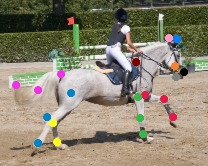
\includegraphics[width=.24\linewidth]{annotations/00110_rgb_horse_cropped.jpg}
  ~
  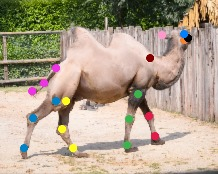
\includegraphics[width=.24\linewidth]{annotations/00021_camel_rgb_cropped.jpg}
  ~
  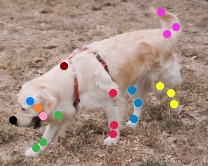
\includegraphics[width=.24\linewidth]{annotations/00085_rgb_dog_cropped.jpg}
  ~
  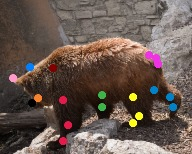
\includegraphics[width=.24\linewidth]{annotations/00008_bear_rgb_cropped.jpg}}
  \end{center}
  \caption{Example joint annotations from the BADJA dataset.  A total of 11 video sequences are in the dataset, annotated every 5 frames with 20 joint positions and visibility indicators.
  }
  \label{fig:badja_examples}
  \end{figure}
  
  
  \subsection{Optimal joint assignment}
  Following non-maximum suppression of the joint heatmaps obtained in Section~\ref{sec:exp-network}, we apply OJA to select an optimal set of joints with which to initialize the final optimization stage. It can be seen that the OJA step is able to address many of the failure cases introduced by the joint prediction network, for example by eliminating physically implausible joint configurations (\figref{comparison}, row 1) or by resolving the ambiguity between the left and right legs (\figref{comparison}, row 2).  Table~\ref{tab:animal} summarizes the performance of both the raw network predictions and results of the two OJA methods. Over most of the sequences in the BADJA dataset it can be seen that the use of coverage terms (employed by the OJA-GA model) improves skeleton accuracy. In particular, the bear, camel and rs\_dog sequences show substantial improvements. The method does however struggle on the horsejump\_high sequence, in which part of the silhouette is occluded by the human rider which adversely affects the silhouette coverage term. Across all sequences the selected OJA-GA method improves joint prediction accuracy by 7\% compared to the raw network output. 
  
  \begin{figure}[t]
  \begin{floatrow}
  \ffigbox{
  \def\bb{\rule{2in}{0pt}\rule{0pt}{1in}}
  \def\comparisonheight{20mm}
  \begin{tabular}{ccc}
    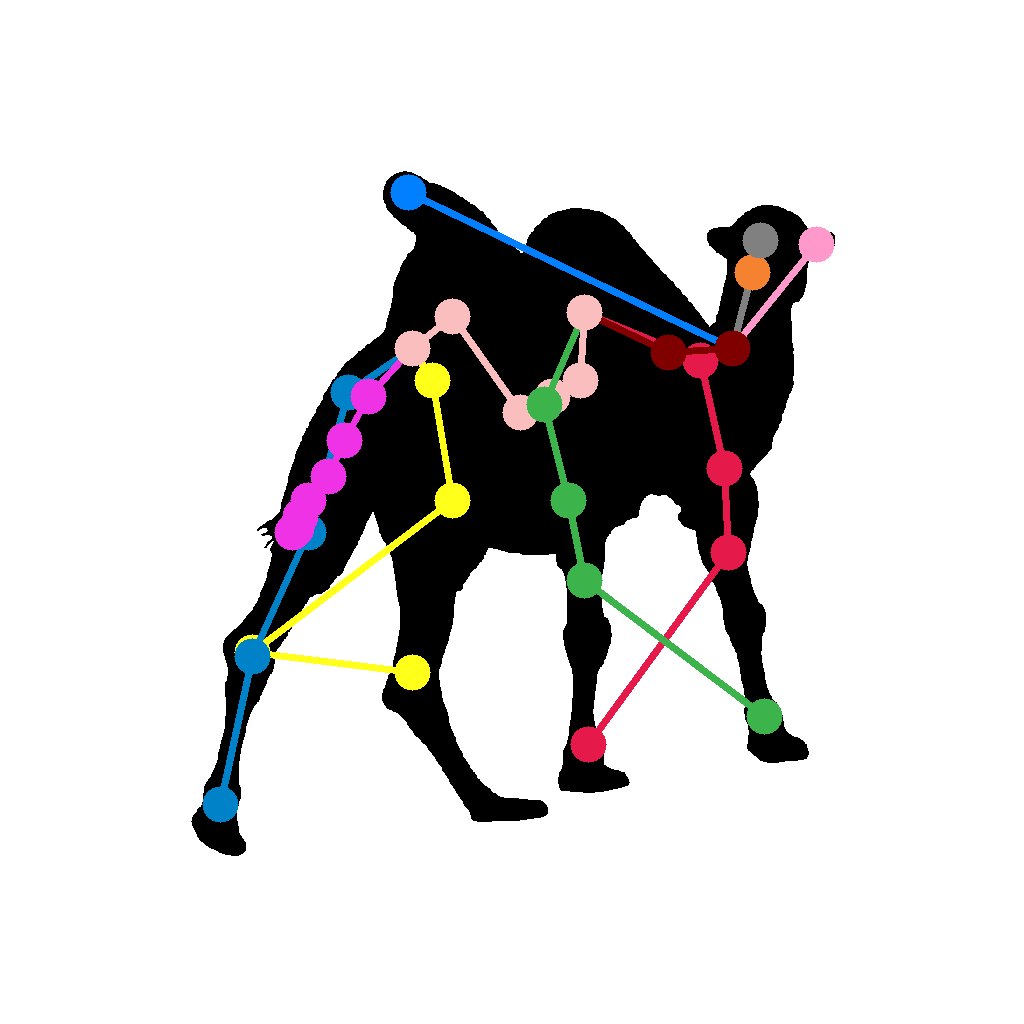
\includegraphics[trim={7cm 6cm 7cm 6cm},clip,height=\comparisonheight]{ga_vs_qp/0046_skel_sil_raw_2.png} &
    
    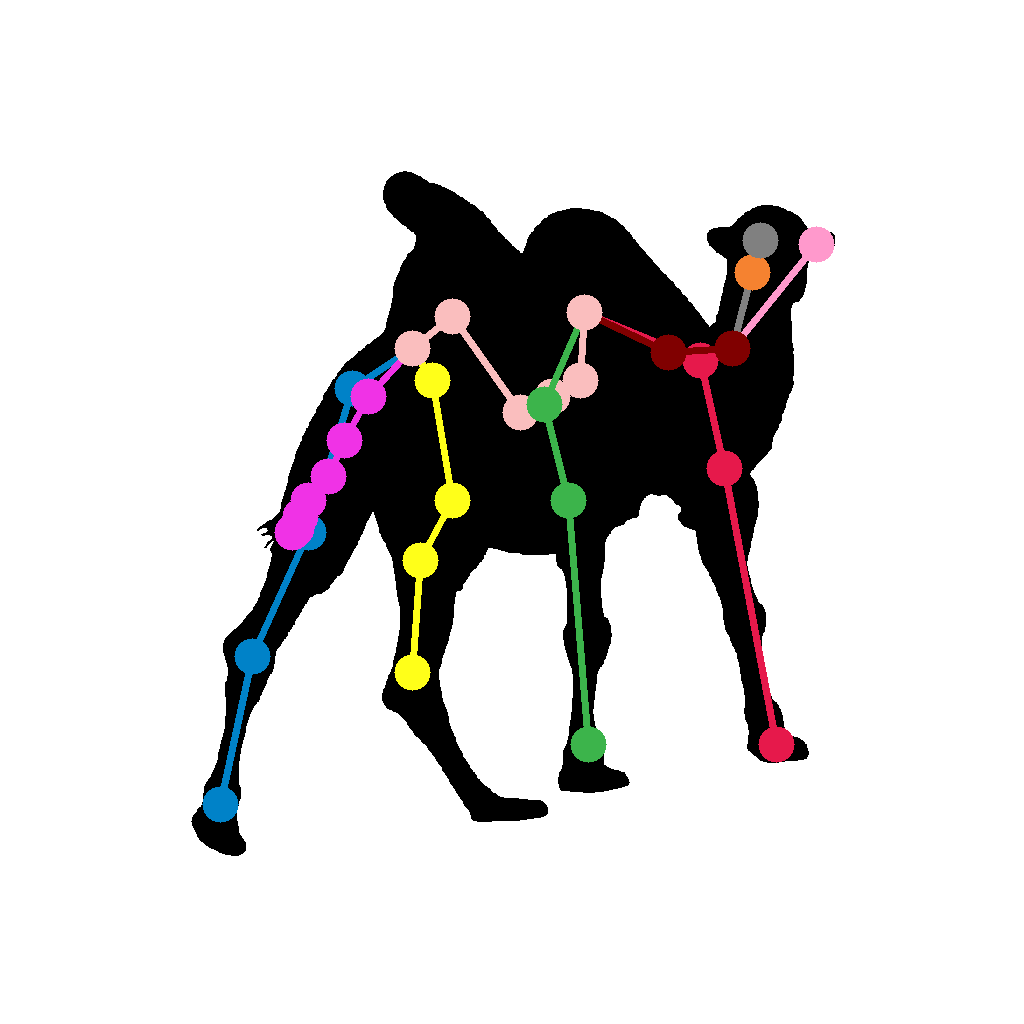
\includegraphics[trim={7cm 6cm 7cm 6cm},clip,height=\comparisonheight]{ga_vs_qp/0046_skel_sil_cleaned_qp_3.png} &
    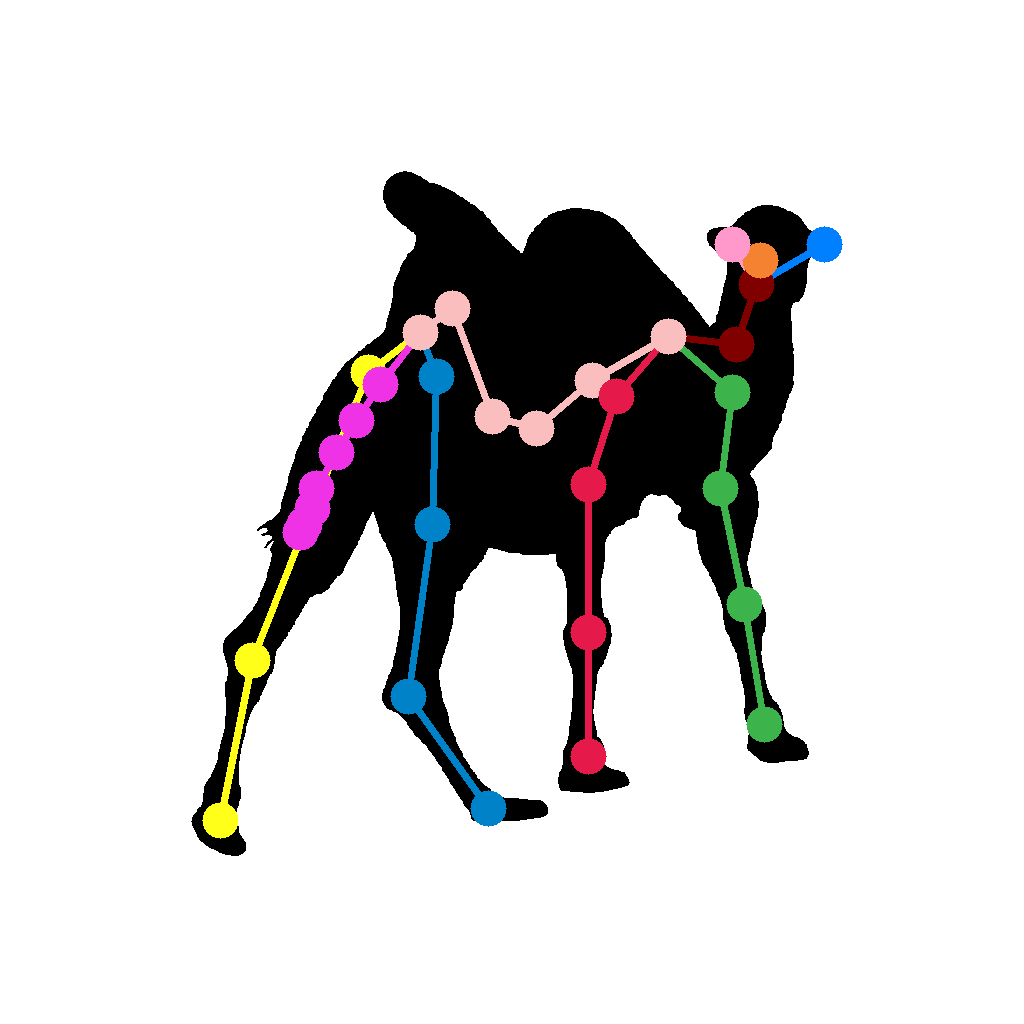
\includegraphics[trim={7cm 6cm 7cm 6cm},clip,height=\comparisonheight]{ga_vs_qp/0046_skel_sil_cleaned_ga_2.png} \\
    
      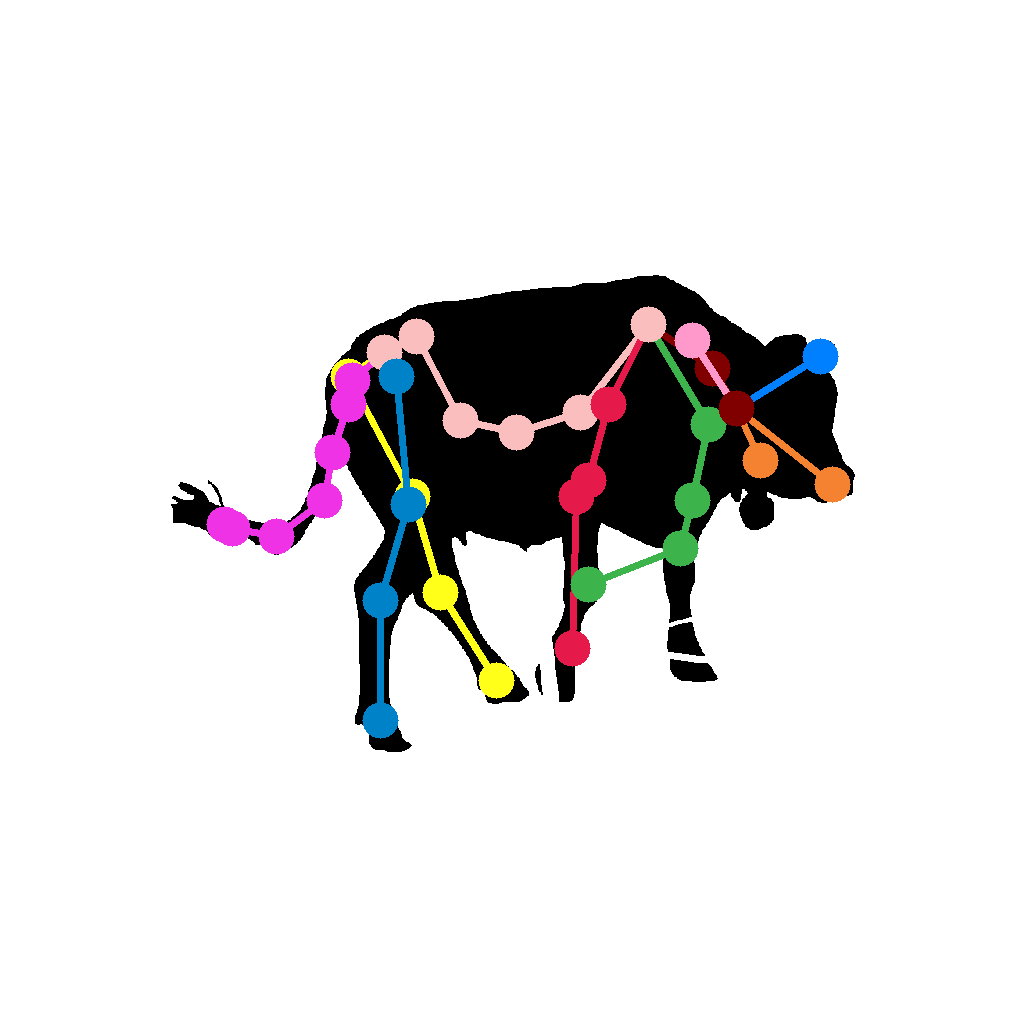
\includegraphics[trim={6cm 6cm 6cm 6cm},clip,height=\comparisonheight]{ga_vs_qp/0069_skel_sil_raw.png}
     &
      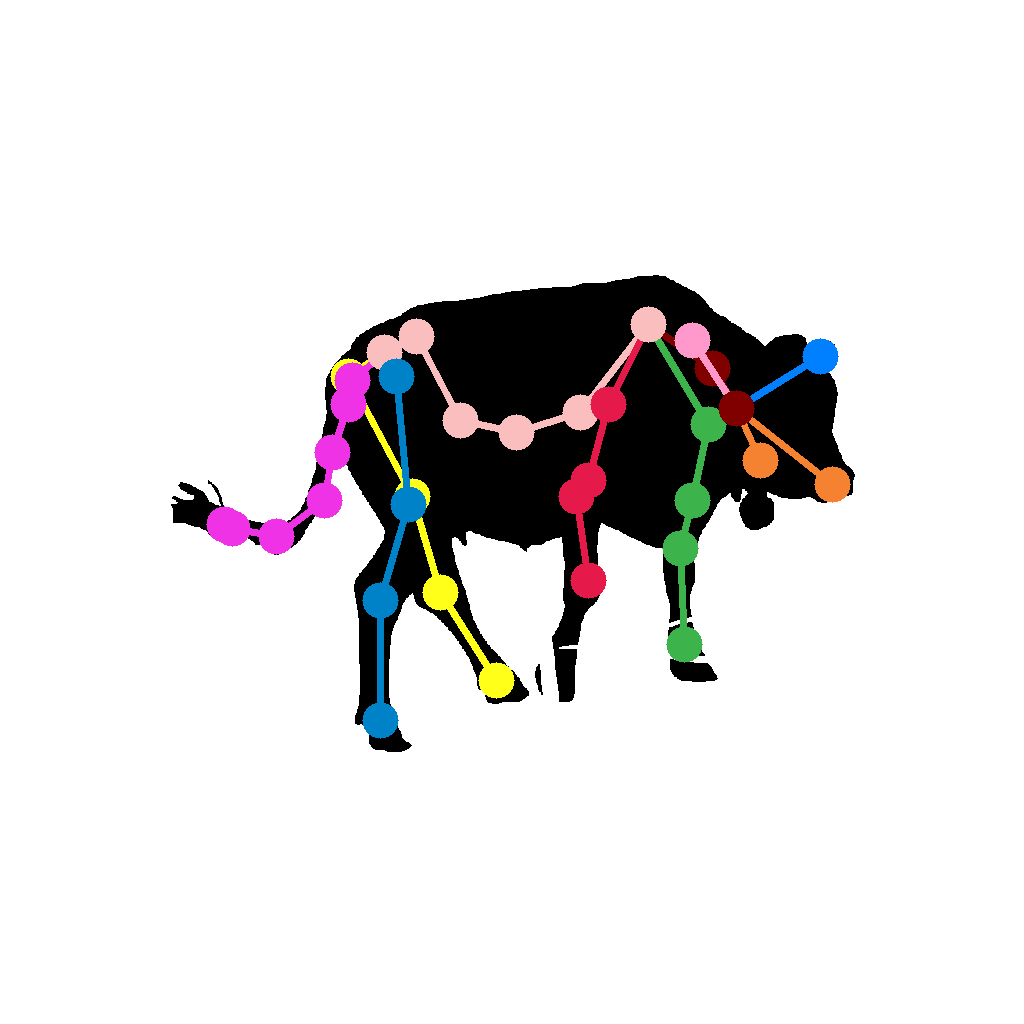
\includegraphics[trim={6cm 6cm 6cm 6cm},clip,height=\comparisonheight]{ga_vs_qp/0069_skel_sil_cleaned_qp.png}
     &
      {}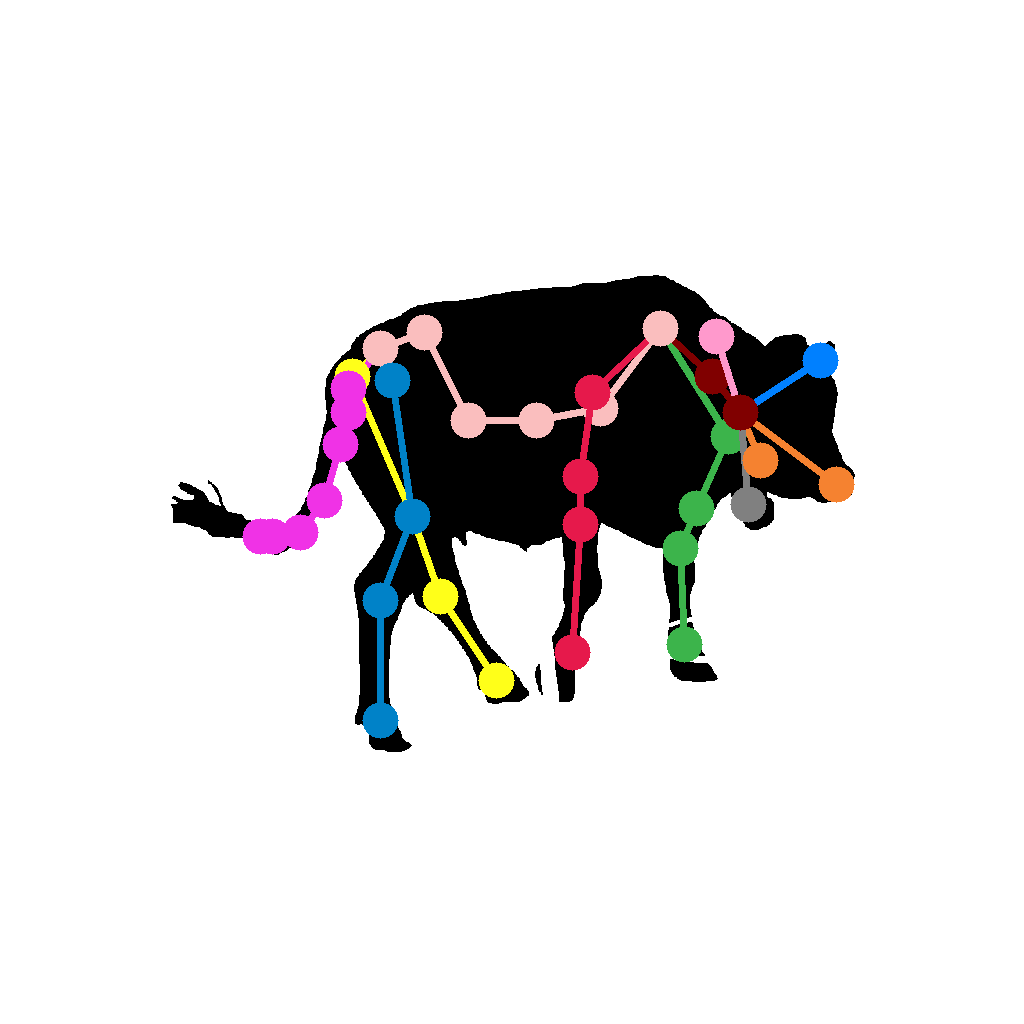
\includegraphics[trim={6cm 6cm 6cm 6cm},clip,height=\comparisonheight]{ga_vs_qp/0069_skel_sil_cleaned_ga.png} \\
      (a) & (b) & (c)
  \end{tabular}
  }{
  \caption{Example skeletons from raw predictions (a), processed with OJA-QP (b), and OJA-GA (c).}
  \label{fig:comparison}
  }
  ~
  \capbtabbox{%
  \small
  \begin{tabular}{lccc}
  \toprule
                 & Raw       & QP        & GA    \\
  \midrule
  bear           & 83.1      & 83.7      & \textbf{88.9}   \\
  camel          & 73.3      & 74.1      & \textbf{87.1}   \\
  cat            & 58.5      & \textbf{60.1}      & 58.4    \\
  cows           & 89.2      & 88.4      & \textbf{94.7}  \\
  dog            & \textbf{66.9}  & 66.6   & \textbf{66.9}  \\
  horsejump-high & 26.5      & \textbf{27.7}      & 24.4   \\
  horsejump-low  & 26.9      & 27.0      & \textbf{31.9}   \\
  tiger          & 76.5      & 88.8      & \textbf{92.3}   \\
  rs\_dog        & 64.2      & 63.4      & \textbf{81.2}   \\
  \midrule
  Average        & 62.8      & 64.4      & \textbf{69.5}   \\
  \bottomrule
  \end{tabular}
  }{\caption{Accuracy of OJA on BADJA test sequences.}
  \label{tab:animal}
  }
  \end{floatrow}
  \end{figure}
  
  \begin{table}[ht]
  \centering
  \small
  \begin{tabular}{@{}cccccccccc@{}}
  
  \toprule
         \multirow{2}{*}{Seq.}  & \multirow{2}{*}{Family} & \multicolumn{2}{c}{PCK (\%)} &   \multirow{2}{*}{Mesh}  & \multirow{2}{*}{Seq.} & \multirow{2}{*}{Family} & \multicolumn{2}{c}{PCK (\%)} &   \multirow{2}{*}{Mesh} \\
  &  & Raw                  & OJA-GA &  &&& Raw                  & OJA-GA           \\ \midrule
  01 & Felidae         & 91.8     & 91.9  & 38.2   &  06 & Equidae         & 84.4     & 84.8  & 19.2     \\
  02 & Felidae         & 94.7     & 95.0  & 42.4   &  07 & Bovidae         & 94.6     & 95.0  & 40.6     \\
  03 & Canidae         & 87.7     & 88.0  & 27.3   &  08 & Bovidae        & 85.2     & 85.8  & 41.5     \\  
  04 & Canidae         & 87.1     & 87.4  & 22.9   &  09 & Hippopotamidae  & 90.5     & 90.6  & 11.8     \\
  05 & Equidae         & 88.9     & 89.8  & 51.6   &  10 & Hippopotamidae  & 93.7     & 93.9  & 23.8     \\    
  \bottomrule
  \end{tabular}%
  
  \caption{Quantitative evaluation on synthetic test sequences. We evaluate the performance of the raw network outputs and quadratic program post-processing using the probability of correct keypoint (PCK) metric (see sec. \ref{sec:exp-network}). We evaluate mesh fitting accuracy by computing the mean distance between the predicted and ground truth vertices.}
  \label{tab:synthetic}
  \end{table}
  
  \begin{figure}[t]
  \def\bb{\rule{2in}{0pt}\rule{0pt}{1in}}
  \def\bjb{\rule{0.5in}{0pt}\rule{0pt}{0.25in}}
  \setlength{\fboxsep}{0pt}%
  \centering
  \begin{tabular}{ccc}
  \includegraphics[width=0.3\linewidth]{smal_comp_cat/rgb_cropped.jpg}
  &
  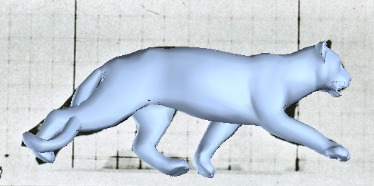
\includegraphics[width=0.3\linewidth]{smal_comp_cat/muybridge_107_smal_res_cropped.jpg}
  &
  \includegraphics[width=0.3\linewidth]{smal_comp_cat/3d_fit_overlay_rgb_cropped.jpg}
  \\
  
  \includegraphics[width=0.3\linewidth]{smal_comp_horse/rgb_cropped.jpg} &
  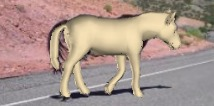
\includegraphics[width=0.3\linewidth]{smal_comp_horse/00049424_ferrari_smal_cropped.jpg} &
  
  \includegraphics[width=0.3\linewidth]{smal_comp_horse/3d_fit_overlay_rgb_cropped.jpg} \\
  
  RGB & SMAL \cite{zuffi2017menagerie} & \textbf{Ours}
  \end{tabular}
  \caption{Our results are comparable in quality to SMAL~\cite{zuffi2017menagerie}, but note that we do not require hand-clicked keypoints.
  }
  \label{fig:compar_smal}
  \end{figure}
  
  \subsection{Model fitting}
  The predicted joint positions and silhouette are input to the optimization phase, which proceeds in four stages. The first stage solves for the model's global rotation and translation parameters, which positions the camera. We follow SMPLify~\cite{bogo2016keep} by solving this camera stage for torso points only, which remain largely fixed through shape and pose variation. We then solve for all shape, pose and translation parameters and gradually decrease the emphasis of the priors. The silhouette term is introduced in the penultimate stage, as otherwise we find this can lead to the optimizer finding unsatisfactory local minima.
  
  The final outputs of our optimization pipeline are shown in \figref{example_results}. In each of the cases illustrated the optimizer is able to successfully find a set of pose and shape parameters which, when rendered, closely resembles the input image. The final row of \figref{example_results} demonstrates the generalizability of the proposed method: the algorithm is able to find a reasonable pose despite no camel figurines being included in the original SMAL model.
  
  \subsubsection*{Comparison to other work.} We compare our approach visually to that given by Zuffi {\em et al.}~\cite{zuffi2017menagerie}. Recall that their results require hand-clicked keypoints whereas ours fits to points predicted automatically by the hourglass network, which was trained on synthetic animal images. Further, their work is optimized for single frame fitting and is tested on animals in simple poses, whereas we instead focus on the more challenging task of tracking animals in video. \figref{compar_smal} shows the application of our model to a number of single frame examples from the SMAL result data~\cite{zuffi2017menagerie}.
  
  \subsubsection*{Quantitative experiments.}
  There is no existing ground truth dataset for comparing reconstructed 3D animal meshes, but an estimate of quantitative error is obtained by testing on synthetic sequences for a range of quadruped species. These are generated by randomly deforming the model and varying the camera position to animate animal motion, see Figure~\ref{fig:synth}. Table~\ref{tab:synthetic} shows results on these sequences. 
  %bjb_insert
  
  \begin{figure}[t!]
  \begin{tabular}{cccccc}
  \includegraphics[width=0.16\linewidth]{synth_pipeline_45/gt_fit_cropped.png} & 
  \includegraphics[width=0.16\linewidth]{synth_pipeline_45/3d_fit_cropped.png} &
  
  \includegraphics[width=0.16\linewidth]{synth_pipeline_50/gt_fit_cropped.png} &
  \includegraphics[width=0.16\linewidth]{synth_pipeline_50/3d_fit_cropped.png} &
  
  \includegraphics[width=0.16\linewidth]{synth_pipeline_55/gt_fit_cropped.png} &
  \includegraphics[width=0.16\linewidth]{synth_pipeline_55/3d_fit_cropped.png} \\
  \end{tabular}
  \caption{Evaluating synthetic data. Green models: ground truth, Orange models: predicted. Frames 5, 10 and 15 of sequence 4 shown. Error on this sequence 22.9.}
  \label{fig:synth}
  \end{figure}
  
  \subsection{Automatic silhouette prediction}
  While not the main focus of our work, we are able to perform the full 3D reconstruction process from an input image with no user intervention. We achieve this by using the DeepLabv3+ network~\cite{deeplabv3plus} as a front-end segmentation engine to automatically generate animal silhouettes. This network was trained on the PASCAL VOC 2012 dataset, which includes a variety of animal quadruped classes. An example result generated using the fully automatic pipeline is shown in \figref{overview}.
  
  \clearpage
  
  \begin{figure}[h!]
  \def\bb{\rule{2in}{0pt}\rule{0pt}{1in}}
  \def\lp#1[#2]#3{\parbox{0.16\linewidth}{\labelledpic{#1}{\includegraphics[#2]{#3}}}}
  \begin{tabular}{cccccc}
  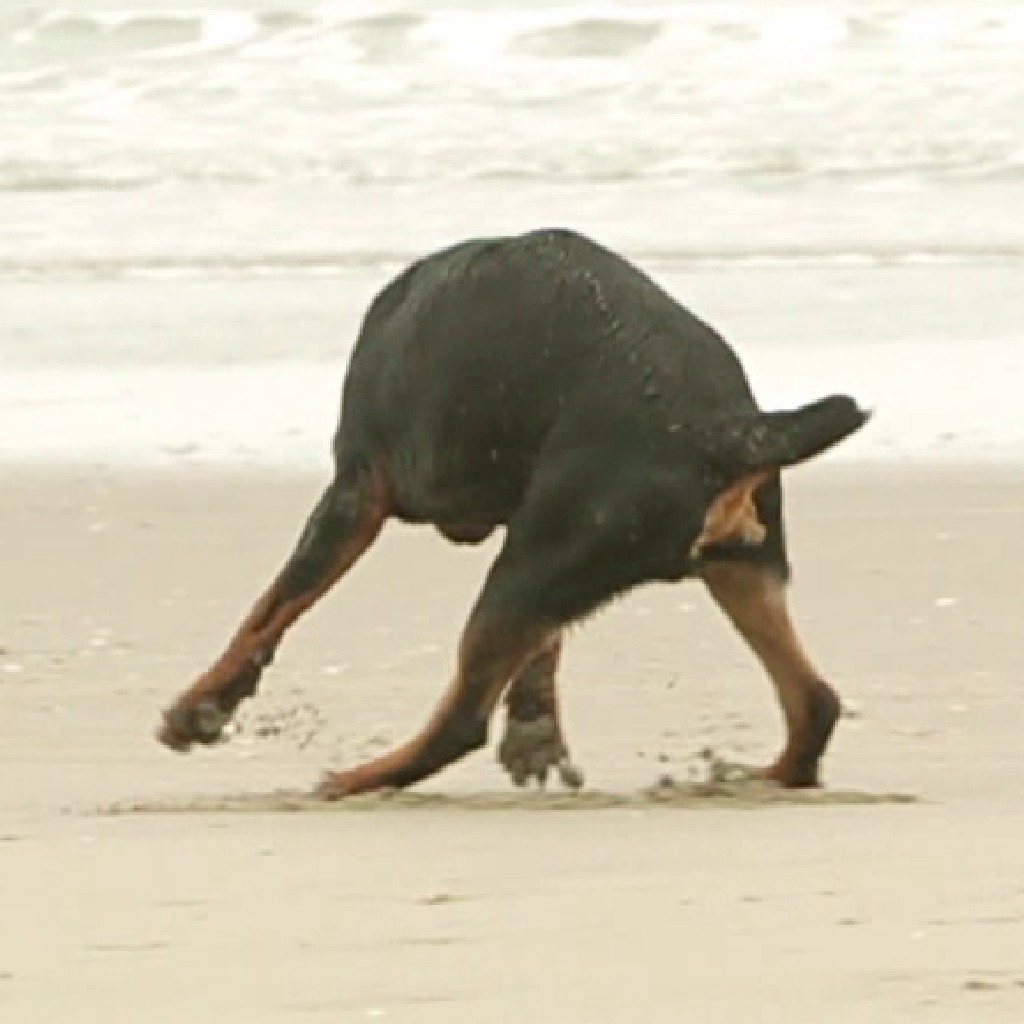
\includegraphics[trim={0 2cm 0 1.25cm},clip,width=0.16\linewidth]{res_bear_new/rgb.jpg} & 
  
\includegraphics[trim={0 2cm 0 1.25cm},clip,width=0.16\linewidth]{res_bear_new/target.jpg} & 
  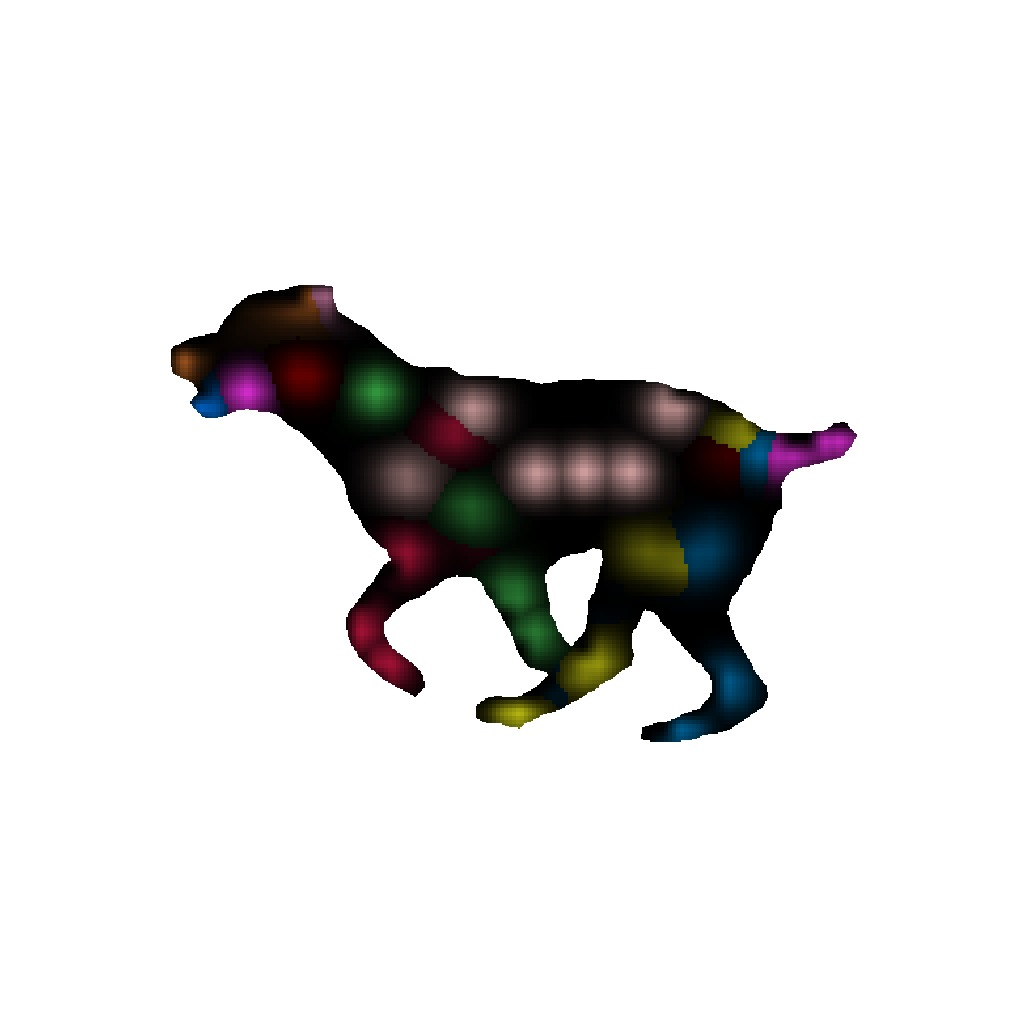
\includegraphics[trim={0 2cm 0 1.25cm},clip,width=0.16\linewidth]{res_bear_new/heatmap.jpg} & 
  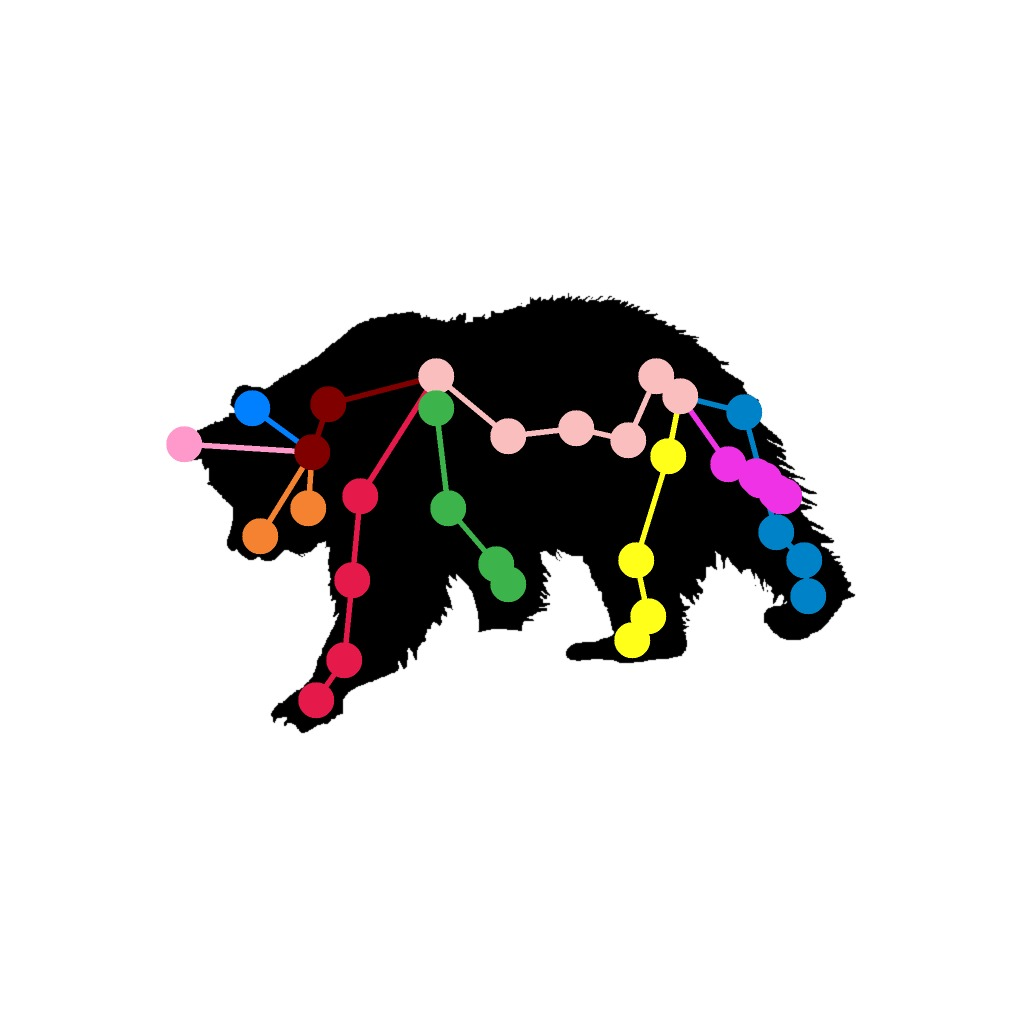
\includegraphics[trim={0 2cm 0 1.25cm},clip,width=0.16\linewidth]{res_bear_new/cleaned_skeleton_sil.jpg} &
  \includegraphics[trim={0 2cm 0 1.25cm},clip,width=0.16\linewidth]{res_bear_new/3d_fit_overlay_rgb.jpg} & 
  \includegraphics[trim={0 2cm 0 1.25cm},clip,width=0.16\linewidth]{res_bear_new/3d_fit_reversed.jpg} \\
  
  \includegraphics[trim={0 0.5cm 0 0.5cm},clip,width=0.16\linewidth]{res_horse_new/rgb.jpg} & 
  \includegraphics[trim={0 0.5cm 0 0.5cm},clip,width=0.16\linewidth]{res_horse_new/target.jpg} & 
  \includegraphics[trim={0 0.5cm 0 0.5cm},clip,width=0.16\linewidth]{res_horse_new/heatmap.jpg} & 
  \includegraphics[trim={0 0.5cm 0 0.5cm},clip,width=0.16\linewidth]{res_horse_new/cleaned_skeleton_sil.jpg} &
  \includegraphics[trim={0 0.5cm 0 0.5cm},clip,width=0.16\linewidth]{res_horse_new/3d_fit_overlay_rgb.jpg} & 
  \includegraphics[trim={0 0.5cm 0 0.5cm},clip,width=0.16\linewidth]{res_horse_new/3d_fit_reversed.jpg} \\
  
  \includegraphics[trim={0 1.5cm 0 1.5cm},clip,width=0.16\linewidth]{res_rsdog158_new/rgb.jpg} & 
  \includegraphics[trim={0 1.5cm 0 1.5cm},clip,width=0.16\linewidth]{res_rsdog158_new/target.jpg} & 
  \includegraphics[trim={0 1.5cm 0 1.5cm},clip,width=0.16\linewidth]{res_rsdog158_new/heatmap.jpg} & 
  \includegraphics[trim={0 1.5cm 0 1.5cm},clip,width=0.16\linewidth]{res_rsdog158_new/cleaned_skeleton_sil.jpg} &
  \includegraphics[trim={0 1.5cm 0 1.5cm},clip,width=0.16\linewidth]{res_rsdog158_new/3d_fit_overlay_rgb.jpg} & 
  \includegraphics[trim={0 1.5cm 0 1.5cm},clip,width=0.16\linewidth]{res_rsdog158_new/3d_fit_reversed.jpg} \\
  
  \lp a[trim={0 1cm 0 1cm},clip,width=0.98\linewidth]{res_camel_new/rgb.jpg} & 
  \lp b[trim={0 1cm 0 1cm},clip,width=0.98\linewidth]{res_camel_new/target.jpg} & 
  \lp c[trim={0 1cm 0 1cm},clip,width=0.98\linewidth]{res_camel_new/heatmap.jpg} & 
  \lp d[trim={0 1cm 0 1cm},clip,width=0.98\linewidth]{res_camel_new/cleaned_skeleton_sil.jpg} &
  \lp e[trim={0 1cm 0 1cm},clip,width=0.98\linewidth]{res_camel_new/3d_fit_overlay_rgb.jpg} & 
  \lp f[trim={0 1cm 0 1cm},clip,width=0.98\linewidth]{res_camel_new/3d_fit_reversed.jpg} 
  \end{tabular}
  \caption{Example results on various animals. From left to right: RGB input, extracted silhouette, network-predicted heatmaps, OJA-processed joints, overlay 3D fit and alternative view.}
  \label{fig:example_results}
  \end{figure}
  
  \vspace{-3em}
  
  \begin{figure}[h!]
  \centering
  \def\p#1{\includegraphics[trim={0 1cm 0 1cm},clip,height=0.12\linewidth] {dog_agility_blooper/#1.jpg}}
  \p{target}
  \p{3d_fit_overlay_rgb}
  \def\p#1{\includegraphics[trim={0 1cm 0 1cm},clip,height=0.12\linewidth] {elephant_blooper/#1.jpg}}
  \p{target}
  \p{3d_fit_overlay_rgb}
  \def\p#1{\includegraphics[trim={0 1cm 0 1cm},clip,height=0.12\linewidth] {rhino_blooper/#1.jpg}}
  \p{target}
  \p{3d_fit_overlay_rgb}
  
  \caption{Failure modes of the proposed system. \emph{Left}: Missing interior contours prevent the optimizer from identifying which way the dog is facing. \emph{Middle}: The model has never seen an elephant, so assumes the trunk is the tail. \emph{Right}: Heavy occlusion. The model interprets the tree as background and hence the silhouette term tries to minimize coverage over this region.}
  \label{fig:blooper}
  \end{figure}
  
  \vspace{-2em}
  \section{Conclusions}
  In this work we have introduced a technique for 3D animal reconstruction from video using a quadruped model parameterized in shape and pose. By incorporating automatic segmentation tools, we demonstrated that this can be achieved with no human intervention or prior knowledge of the species of animal being considered. Our method performs well on examples encountered in the real world, generalizes to unseen animal species and is robust to challenging input conditions.
  



%!TEX root = ../thesis.tex
%*******************************************************************************
%****************************** Third Chapter **********************************
%*******************************************************************************
\chapter{Learning from Synthetic Data; Bridging the Domain Gap}\label{chap:cgas}

\def\figref#1{Fig.~\ref{fig:#1}}

% **************************** Define Graphics Path **************************
\ifpdf
    \graphicspath{{Chapter4/Figs/Raster/}{Chapter4/Figs/PDF/}{Chapter4/Figs/}}
\else
    \graphicspath{{Chapter4/Figs/Vector/}{Chapter4/Figs/}}
\fi

% Plan:
% - Introduction - complain about the non-automatic equivalent systems & lack of training data for animals. Impractical to obtain. 
% - Begin with a discussion on systems that use synthetic data for training. Related work should focus on these
% - Discuss methods for generating accurate synthetic data, particularly focus on SURREAL. 
% - Create experiments in which different methods are trained and tested on varying levels of fake data.
% - In-depth explanation of synthetic data creation
% - In-depth explanation of training the joint predictor. Possibly ablate the sampling strategy / architecture. Diagrams etc.
% - Explain why we need to fix with a QP/GA.
% - In depth formulation of the QP and show it works, then explain the GA.
% - Experimental evaluation -- in depth explanation about the data collection exercise etc.
% - Experimental comparison between the two methods
% - In-depth explantion of the SMAL optimizer.
% - Results and comparison to related work
% - Summary 

% Extra experiments: 
% (1) Show that training on synthetic real data doesn't work (e.g. fake textures).
% (2) Use a GAN to generate synthetic data? Why not? Articulated sections didn't work.

\section{Introduction}

    This chapter introduces a system for recovering the 3D shape and motion of a wide variety of quadrupedial animals from video. Inspired by techniques from the recent human body and hand tracking literature (most notably SMPLify~\cite{bogo16keep}), the system comprises a machine learning front-end for predicting 2D joint positions followed by an energy minimization stage which fits a detailed 3D model to the image. However, this chapter will discuss a number of key challenges which arise when reconstructing animal subjects compared with humans and methods to overcome them.

\subsection{Limited animal training data}
    For human tracking, hand labelled sequences of 2D segmentations and joint positions have been collected from a wide variety of sources~\cite{andriluka14cvpr,lin2014microsoft,johnson2010clustered}. Of these two classes of labelling, animal {\em segmentation} data is available in datasets such as MSCOCO~\cite{lin2014microsoft}, PASCAL VOC~\cite{everingham2010pascal} and DAVIS~\cite{Perazzi2016}.  However this data is considerably sparser than human data, and must be ``shared'' across species, meaning the number of examples for a given animal shape class is considerably fewer than is available for an equivalent variation in human shape.  While segmentation data can be supplied by non-specialist human labellers, it is more difficult to obtain {\em joint position} data.  Some joints are easy to label, such as ``tip of snout'', but others such as the analogue of ``right elbow'' require training of the operator to correctly identify across species. In the case of SMPLify, the network is trained on large-scale human keypoint datasets, including MPII~\cite{andriluka14cvpr} (approx. 40,000 people) and the Leeds Sport Dataset~\cite{johnson2010clustered}. Unfortunately, there is no keypoint dataset for animals that cover even a small fraction of the quadruped types that we aim to reconstruct. 

    Of greater concern however, is 3D skeleton data.  For humans, motion capture (mocap) can be used to obtain long sequences of skeleton parameters (joint positions and angles) from a wide variety of motions and activities. For animal tracking, this is considerably harder: animals behave differently on treadmills than in their quotidian environments, and although some animals such as horses and dogs have been coaxed into motion capture studios~\cite{wilhelm2015furyexplorer}, it remains impractical to consider mocap for a family of tigers at play.

    These dataset challenges have, at least in part, resulted in the lack of \emph{automatic} approaches for 3D animal reconstruction. Precisely, prior to the design of the system discussed in this chapter, 3D animal reconstruction techniques relied on at least one of manually provided silhouettes, keypoint locations or limb tracks. The techniques are summarized in \Cref{tab:animal-annot-tab} and discussed in depth in \Cref{chap:relwork}. 

    

% \newcommand{\awfhang}[1]{
%     \begin{minipage}[t]{\textwidth}% Top-hanging minipage, will align on
%                                    % bottom of first line
%     \begin{tabbing} % tabbing so that minipage shrinks to fit
%     \\[-\baselineskip] % Make first line zero-height
%     #1 % Include user's text
%     \end{tabbing}
%     \end{minipage}} % can't allow } onto next line, as {WIDEBOX}~x will not tie.
    
    \newcolumntype{L}[1]{>{\RaggedRight\hspace{0pt}}p{#1}}
    \newcolumntype{R}[1]{>{\RaggedLeft\hspace{0pt}}p{#1}}
    
    \begin{table}[t!]
    {\sffamily
    \scriptsize
    \def\hd#1{\awfhang{#1}}
    \begin{tabular}{@{}L{20mm}%Paper
    L{10mm}%Year
    |L{12mm}%Class
    L{15mm}%Train
    |L{15mm}%Template
    L{17mm}%Video
    L{17mm}%Test
    |L{9mm}%Model
    L{5mm}%Size
    @{}}
    \hd{Paper}%
    &\hd{Release\\Year}%
    &\hd{Animal\\Class}%
    &\hd{Training\\requirements}%
    &\hd{Template\\Model}%
    &\hd{Video\\required}%
    &\hd{Test Time\\Annotation}%
    &\hd{Model\\Fitting}%
    &\hd{Test\\Size}%
    \\\hline
    %%%%%%%%%%%%%%%%%%%%%%
    What Shape are Dolphins~\cite{cashman2013shape}
    & 2013
    & Dolphins, Pigeons 
    & Not trained
    & Dolphin Template
    & 25 frames / category & J2, S2 & Yes & 25
    \\\hline
    %%%%%%%%%%%%%%%%%%%%%%
    Animated 3D Creatures~\cite{reinert2016animatedsketching}
    & 2016
    & MLQ
    & Not trained
    & Generalized Cylinders
    & Yes & J2, S2 & Yes & 15
    \\\hline
    %%%%%%%%%%%%%%%%%%%%%%
    3D Menagerie (SMAL)~\cite{zuffi2017menagerie}       
    & 2017         
    & MLQ 
    & Not trained
    & SMAL
    & No & J2, S2 & Yes & 48 
    \\\hline
    %%%%%%%%%%%%%%%%%%%%%%
    Category Specific Mesh Reconstructions~\cite{kanazawa2018birds}
    & 2018
    & Birds
    & J2, S2
    & Bird convex hull
    & No & None & No & 2850          
    \\\hline
    %%%%%%%%%%%%%%%%%%%%%%
    Lions, Tigers and Bears (SMALR)~\cite{zuffi_lions} 
    & 2018
    & MLQ
    & Not trained
    & SMAL
    & 3-7 frames / animal & J2, S2 & Yes & 14
    \\\hline
    %%%%%%%%%%%%%%%%%%%%%%
    This paper
    & 2018
    & MLQ
    & Not trained
    & SMAL
    & Yes & S2 (for best results shown) & Yes & 9
    \\\hline 
    %%%%%%%%%%%%%%%%%%%%%%
    Who Left the Dogs Out?
    & 2018
    & Dogs  % 2D Joints, Silhouettes, 3D Template, 3D Priors
    & J2, S2, T3, P3
    & SMAL
    & No & None & No & 1703
    \\\hline
    %%%%%%%%%%%%%%%%%%%%%%
    3D-Safari~\cite{Zuffi19Safari}        
    & 2019
    & Zebras, horses
    % 3D models (albeit synthetic), 2D Joints,  Silhouettes,  3D Priors
    & M3 (albeit synthetic), J2, S2, P3
    & SMAL
    & 3-7 frames / animal & None & Yes & 200
    \\\hline
    %%%%%%%%%%%%%%%%%%%%%%
    U-CMR~\cite{Zuffi19Safari}        
    & 2020
    & Birds
    % 3D models (albeit synthetic), 2D Joints,  Silhouettes,  3D Priors
    & M3 (albeit synthetic), J2, S2, P3
    & Bird convex hull
    & 3-7 frames / animal & None & Yes & 200
    \\\hline
    \end{tabular}
    }
    \caption{Literature summary: Analysis of required input annotations.
    MLQ: Medium-to-large quadrupeds. J2: 2D Joints. S2: 2D Silhouettes. T3: 3D Template. P3: 3D Priors. M3: 3D Model.}
    \label{tab:animal-annot-tab}
    % \vspace{-8mm}
    \end{table}
    
    


\subsection{Synthetic image generation}

    In the absence of real-world motion capture data, the recent publication of the Skinned Multi-Animal Linear (SMAL) model~\cite{zuffi2017menagerie} offers a method for \emph{synthetic} data generation. Analogous in design to the popular SMPL~\cite{loper15smpl} parametric human model, SMAL can generate a wide range of quadruped species. As discussed in \Cref{chap:relwork}, SMAL overcomes the lack of 3D animal training data by instead learning from 41 scans of toy figurines. This results in SMAL being of considerably lower fidelity than the SMPL, which was constructed from 1786 3D human scans. However, the model's PCA shape space offers a mechanism for sampling potentially infinite quadruped animals of satisfactory realism which can form a valuable training dataset.
    
    % comes without surface texture maps. 
    The use of synthetic images to train 3D reconstruction systems has been attempted in recent computer vision literature. The general approach is to capture training images by capturing multiple images of a representative 3D model (or scene) by randomly sampling camera and environmental parameters. A machine learning model is then trained on this dataset $D_{synth}$ of synthetic images and later tested on a dataset $D_{real}$ of real-world examples. This procedure offers an important practical advantage; the training images can be automatically generated with correponding annotations. Depending on the task, this can overcome a lengthy and complex process of sourcing manual annotations from users. However, designing a data pipeline which can generate synthetic images with sufficient realism to be representative of real test images $D_{real}$ is challenging. A common pitfall of such approaches is the tendancy to train machine learning models that perform well on unseen synthetic images but poorly on real world examples. This phenomenon is often caused by systematic differences between the $D_{synth}$ and $D_{real}$, resulting in the model becoming overreliant on features present only in $D_{synth}$ or unfamiliar with features present only in $D_{real}$. The differences between datasets is often described as the \emph{domain gap} which must be bridged in order to achieve a successful predictor. 

    %Review paper: https://arxiv.org/pdf/1909.11512.pdf?fbclid=IwAR2FuZvNAlIGuyh2wtVEmj_rLzjaJvCjMNWP_svBqhMtnXcEX-NV9z8rR7g
    Fortunately, there are a number of options for tackling this problem. A popular strategy is to ensure the generation pipeline is of extremely high quality. SURREAL\lazycite{SURREAL}{SURREAL} is a method which learns from synthetic human images rendered using the popular SMPL~\cite{loper15smpl} parametric model. In this work, the authors go to significant effort to source realistic UV texture maps for SMPL and apply a high quality rendering engine complete with a lighting and reflectance model to generate their training images. A similar approach is followed by SMALST \lazycite{SMALST}{SMALST}, who follow a multi-view optimization pipeline to construct a synthetic zebra training dataset complete with realistic textures. Related also are autonomous driving systems that train (or pre-train) on synthetic `virtual worlds' \lazycite{https://arxiv.org/pdf/1605.06457.pdf?fbclid=IwAR0RtcIEKYgghwD5uo_TSwesiD2XuhqaQtuoTaQe2omp-QCdzJv4O3PjBjU}{Virtual Worlds}. An alternative option is to process the test image dataset to find a representation which is easier to synthesise. For 3D human skeleton prediction, Shotton et al.~\cite{shotton-kinect} synthetise a set of depth images used to train a keypoint regressor. An unfortunate byproduct of this training style however is that it necessitates a depth sensor at test time. 

    %Related also is the work of \lazycite{GTA-Cars}{GTA-Cars} who use a images rendered from a popular video game engine to teach an automous agent to drive with reinforcement learning. 
    %Another category of approaches are found in optical flow. Optical flow is an example of a dense point correspondence task: given two frames $I_{i}, I_{i+1}$ a model should predict a \emph{flow field} $f: \RR{H}{W} \mapsto \RR{H}{W}$. Of course, for this task the most important learning signal is obtained through observing object and camera \emph{motion}. For this reason, multiple models are trained using the FlyingChairs dataset: since natural scenes are complex to generate, models can just learn from flow directly. % Tidy up this argument

    A significant advance has been made recently with the introduction of generative adversarial networks (GANs). The idea of a GAN is to train two `competing' networks: the \emph{generator} is tasked with producing synthetic images and the \emph{discriminator} determines if a given input image originated in a real-world dataset or was instead synthesized by the generator. These two networks are given opposite goals: the generator is penalized if it fails to `fool' the discriminator, and the discriminator is penalized if it fails to recognize a synthesized image. By training these networks jointly, the generator eventually learns to produce synthetic images of extremely high quality, since the discriminator provides feedback on even subtle aspects of the synthetic images which are unreaslistic. Despite the remarkable quality of `GANerated' images, the challenge of conditioning GANs to generate \emph{structured} images is still an evolving field. For example, a sensible challenge might be to train a GAN to generate UV texture maps for the SMAL model. 
    
    
    of this is that there should be an analoug% TODO: Justify why GANs are a bad idea...
    % Mode collapse
    % With GANs, there should be an anology between shapes in the real and synthetic set. However, it's difficult to render synthetic shapes which match shapes in an unlabelled test dataset. 
    
    The system presented in this section adopts an alternative (and much simpler) approach for synthetic image generation. The idea builds on the realisation that a 2D silhouette image encodes a significant amount of the object's shape features, and by virtue of being textureless and having no background detail is much simpler to synthesise. As previously discussed, there are also a great number of `off-the-shelf' image segmentation engines which can produce accurate animal silhouettes of a high quality. 

    The joint candidate predictor is trained on synthetically generated silhouette images, and at test time, deep learning methods or standard video segmentation tools are used to extract silhouettes from real data. The system is tested on animal videos from several species, and shows accurate reconstructions of 3D shape and pose.


\subsection{Handling silhouette ambiguity}

    An unfortunate drawback of using silhouette images (for example, when compared to RGB or depth counterparts) is that missing interior contours leads to a source of reconstruction ambiguity. An example of this is shown in Figure 6 in which two distinct 3D reconstructions are shown to yield similar 2D silhouette reprojections. Clearly, a naive joint predictor which regreses a single set of 2D coordinates from an input silhouette would perform suboptimally, since the silhouette alone contains insufficient information to resolve such cases. 

    However, the fact that the system is designed to accept a video sequence as input (rather than a single frame) provides additional information which can be used to resolve per-frame ambiguities. This section describes a method for incoporating temporal knowledge in order to obtain a reliable set of predicted 2D joint coordinates that later form the basis for the 3D model fitting stage. The key insight is to modify a standard joint heatmap predictor~\lazycite{hourglassnet} {hourglassnet} in order to encourage multi-modal outputs, both when trained on synthetic data and later tested on real world frames. A novel discrete optimization stage is then used to recover the skeleton trajectory of maximal likelihood from the sequence of multi-modal predictions. This section will explore two methods for achieving this: the first frames the problem as a quadratic program and the later provides achieves a significant efficiency improvement by using a genetic algorithm. 


%The system comprises a machine learning front-end which predicts candidate 2D joint positions, a discrete optimization which finds kinematically plausible joint correspondences, and an energy minimization stage which fits a detailed 3D model to the image. 


% The core methodologies are inspired by techniques from the recent human body and hand tracking literature, combining machine learning and 3D model fitting. A discriminative front-end uses a deep hourglass network to identify candidate 2D joint positions. These joint positions are then linked into coherent skeletons by solving an optimal joint assignment problem, and the resulting skeletons create an initial estimate for a generative model-fitting back-end to yield detailed shape and pose for each frame of the video.  

% For human tracking, hand labelled sequences of 2D segmentations and joint positions have been collected from a wide variety of sources~\cite{andriluka14cvpr,lin2014microsoft,johnson2010clustered}. Of these two classes of labelling, animal {\em segmentation} data is available in datasets such as MSCOCO~\cite{lin2014microsoft}, PASCAL VOC~\cite{everingham2010pascal} and DAVIS~\cite{Perazzi2016}.  However this data is considerably sparser than human data, and must be ``shared'' across species, meaning the number of examples for a given animal shape class is considerably fewer than is available for an equivalent variation in human shape.  While segmentation data can be supplied by non-specialist human labellers, it is more difficult to obtain {\em joint position} data.  Some joints are easy to label, such as ``tip of snout'', but others such as the analogue of ``right elbow'' require training of the operator to correctly identify across species.

% Of more concern however, is 3D skeleton data.  For humans, motion capture (mocap) can be used to obtain long sequences of skeleton parameters (joint positions and angles) from a wide variety of motions and activities.
% For animal tracking, this is considerably harder: animals behave differently on treadmills than in their quotidian environments, and although some animals such as horses and dogs have been coaxed into motion capture studios~\cite{wilhelm2015furyexplorer}, it remains impractical to consider mocap for a family of tigers at play.

\newfloatcommand{capbtabbox}{table}[][\FBwidth]

\def\bb{\rule{2in}{0pt}\rule{0pt}{1in}}
\def\labelledpic#1#2{
\begin{tikzpicture}
\node (pic) {#1};
\path[fill=white,draw=gray,thick] (pic.south west) +(3ex,3ex) circle (2ex)
   node {#2};
\end{tikzpicture}
}

% TODO!
\begin{figure}[t]
\def\p#1#2{\parbox{0.32\linewidth}{
\labelledpic{\includegraphics[trim={4cm 7cm 4cm 7cm},clip,width=\linewidth]{sys_overview_pred_2/#2.jpg}}
{\scriptsize #1}}}
\def\ps#1#2{\parbox{0.32\linewidth}{
\labelledpic{\includegraphics[trim={0cm 2cm 0cm 2cm},clip,width=\linewidth]{sys_overview_pred_2/#2.jpg}}
{\scriptsize #1}}}
\p a{rgb}             \p b{target}         \p c{heatmap}
\p d{skeleton_sil}    \p e{00048_overlay}  \ps f{00048_alternative}
\caption{{\bf System overview}: input video (a) is automatically processed using DeepLabv3+~\cite{deeplabv3plus} to produce silhouettes (b), from which 2D joint predictions are regressed in the form of heatmaps (c).  Optimal joint assignment (OJA) finds kinematically coherent 2D-to-3D correspondences~(d), 
which initialize a 3D shape model, optimized to match the silhouette~(e). 
Alternative view shown in (f).
}
\label{fig:overview}
\end{figure}

\subsection{Contributions}
Taking into account the above constraints, this work applies a novel strategy to animal tracking, which assumes a machine-learning approach to extraction of animal silhouettes from video, and then fits a parameterized 3D model to silhouette sequences.  The system exhibits the following contributions:
\begin{itemize}
\item A machine-learned mapping from silhouette data of a large class of quadru\-peds to generic 2D joint positions.
\item A novel optimal joint assigment (OJA) algorithm extending the bipartite matching of Cao {\em et al.}~\cite{cao2017realtime} in two ways, one which can be cast as a quadratic program (QP), and an extension optimized using a genetic algorithm (GA).
\item A procedure for optimization of a 3D deformable model to fit 2D silhouette data and 2D joint positions, while encouraging temporally coherent outputs.
\item We introduce a new benchmark animal dataset of joint annotations (BADJA) which contains sparse keypoint labels and silhouette segmentations for eleven animal video sequences. 
Previous work in 3D animal reconstruction has relied on bespoke hand-clicked keypoints~\cite{zuffi2017menagerie,zuffi_lions} and little quantitative evaluation of performance could be given.
The sequences exhibit a range of animals, are selected to capture a variety of animal movement and include some challenging visual scenarios such as occlusion and motion blur.
\end{itemize}
The system is outlined in \figref{overview}.  The remainder of the paper provides a detailed description of system components.  Joint accuracy results at multiple stages of the pipeline are reported on the new BADJA dataset, which contains ground truths for real animal subjects. Experiments are also conducted on synthetic animal videos to produce 3D joint accuracy statistics and full mesh comparisons. A qualitative comparison is given to recent work~\cite{zuffi2017menagerie} on the related single-frame 3D shape and pose recovery problem. The paper concludes with an assessment of strengths and limitations of the work.

% \subsection{Related Work}
% In this section, we will discuss work specifically related to this paper. The broad 

% \subsubsection{Non-automatic approaches for 3D reconstruction of articulated subjects}

% Much of this is handled in the previous section, but could be briefly recapped. Point out that we want an AUTOMATIC technique that can rapidly apply across different quadruped types.

% \subsubsection{Automatic approaches for 3D reconstruction of articulated subjects}

% The SMPLify approach is comprises of two stages, means of achieving 3D human reconstruction. an automatic To train such a system, we may look towards the SMPLify technique employed for 3D human mesh recovery


% \subsubsection{Learning from synthetic data}

% SURREAL dataset for humans. 

% \subsubsection{Cleaning up predictions}

% Talk about pictorial structure models. Could be integrated later.

% \section{Design discussion for an automatic quadruped 3D reconstruction}
% \def\seq#1#2#3#4{\left[{#1_{#2}}\right]_{#2=#3}^{#4}}

% The test-time problem to be solved is to take a sequence of input images and for each image, output the shape, pose and position parameters describing the animal's motion.

% To train such a system, we start by considering the suitability of the SMPLify~\cite{bogo16keep} method (discussed above) which describes a two-stage approach for automatic 3D human reconstruction. However, the approach has particular design requirements that prevents trivial extension to reconstructing quadrupeds. 

% \subsection{Keypoint training data for joint predictor}

% Firstly, the preliminary stage of the approach is based on the DeepCut joint predictor, a convolutional neural network that takes an input an image and predicts a set of semantically meaningful keypoints. In the case of SMPLify, the network is trained on large-scale human keypoint datasets, including MPII~\cite{andriluka14cvpr} (approx. 40,000 people) and the Leeds Sport Dataset~\cite{johnson2010clustered}. As previously discussed, there are no keypoint datasets for animals that cover even a small fraction of the quadruped types that we aim to reconstruct. 

% With no real-world data to use for training the keypoint predictor, we can turn instead to a novel approach that instead relies on synthetic (or fake) data for training. 


% \subsection{Data driven shape and pose priors}

% Of course, we also don't have any shape or pose priors.


\section{Preliminaries}

\subsection{Deformable 3D quadruped model}

This section provides a formal definition for the deformable 3D model that is used to generate synthetic training data and in the model fitting stage to obtain the final mesh. Our system assumes a deformable 3D model such as SMAL~\cite{zuffi2017menagerie} which parametrizes a 3D mesh as a function of {\em pose} parameters~$\pose \in \R\npose$ (e.g.\ joint angles) and {\em shape} parameters~$\shape \in \R\nshape$. 
As discussed in \Cref{chap:relwork}, a 3D mesh is an array of vertices $\verts \in \RR 3\nverts$ (the vertices are columns of a $3 \times \nverts$ matrix) and a set of triangles represented as integer triples $(i,j,k)$, which are indices into the vertex array.
A deformable model such as SMAL may be viewed as supplying a set of triangles, and a function
\begin{equation}
\verts(\pose, \shape) : \R \npose \times \R \nshape \mapsto \RR 3 \nverts
\end{equation}
which generates the 3D model for a given pose and shape.
The mesh topology (i.e.~the triangle vertex indices) is provided by the deformable model, and is the same for all shapes and poses we consider, so in the sequel a mesh will be defined only by the 3D positions of its vertices.

In any given image, the model's 3D {\em position} (i.e.\ translation and orientation) is also unknown, and will be represented by a parametrization $\posn$ which may be for example translation as a 3-vector and rotation in axis angle form. Application of such a transformation to a $3\times\nverts$ matrix will be denoted by $*$, so that 
\begin{equation}
\posn * \verts(\pose, \shape)
\end{equation}
represents a 3D model of given pose and shape transformed to its 3D position.

It is also necessary to define a model's {\em joints}.  These appear naturally in models with an explicit skeleton, but more generally they can be defined as some function mapping from the model parameters to an array of 3D points analogous to the vertex transformation above. Note that even in the case of rigged models, this provides a mechanism to add additional joints beyond the ones required to drive model deformation. In any case, joints are defined by post-multiplying by a $\nverts \times \njoints$ matrix $\jointselect$.  The $j^{\text{th}}$ column of~$\jointselect$ defines the 3D position of joint~$j$ as a linear combination of the vertices (this is quite general, as $\verts$ may include vertices not mentioned in the triangulation).  

\subsection{Camera model, joint reprojection and silhouette rendering}
For both synthetic image generation and the later model fitting stage, it is necessary to be able to \emph{render} the 3D model. A general camera model is described by a function $\proj: \R{3} \mapsto \R{2}$.  This function incorporates details of the camera intrinsics such as focal length, which are assumed known.  
Thus 
\begin{equation} \label{eq:project_joints}
\kappa(\posn, \pose, \shape) := \proj(\posn * \verts(\pose, \shape) \jointselect)
\end{equation}
is the $2\times \njoints$ matrix whose columns are 2D joint locations corresponding to a 3D model specified by (position, pose, shape) parameters $(\posn, \pose, \shape)$.

The model is also assumed to be supplied with a rendering function $R$ which takes a vertex array in camera coordinates, and generates a 2D binary image of the model silhouette.  That is,
\begin{equation} \label{eq:render_sil}
R\bigl(\posn * \verts(\pose, \shape)\bigr) \in \mathbb{B}^{W\times H}
\end{equation}
for an image resolution of $W \times H$.  In order to allow derivatives to be propagated through $R$ (essential for the silhouette term in the model fitting stage), the \emph{differentiable renderer} of Loper et al.~\cite{loper2014opendr} is used. Please see the relevant section in \Cref{chap:relwork} for further details.

\subsection{System overview}

\def\seq#1#2#3#4{\left[{#1_{#2}}\right]_{#2=#3}^{#4}}
The test-time problem to be solved is to take a sequence of input images
\[
\mathcal{I} = \seq{I}{t}{1}{T}
\]
which are segmented to the silhouette of a single animal (i.e.~a video with multiple animals is segmented multiple times), producing a sequence of binary silhouette images 
\[
\mathcal{S} = \seq{S}{t}{1}{T}.
\]

The computational task is to output for each input image the shape, pose, and position parameters describing the animal's motion. Inspired by recent work in human 3D reconstruction, this objective can be broken down into a multiple stage pipeline. 

The core components are as follows:

\begin{enumerate}
    \item The discriminative front-end extracts silhouettes from video, and then uses the silhouettes to predict multi-modal heatmaps, from which 2D joint positions are obtained with multiple candidates per joint. 
    \item Optimal joint assignment (OJA) corrects confused or missing skeletal predictions by finding an optimal assignment of joints from a set of network-predicted proposals. 
    \item Generative deformable 3D model is fitted to the silhouettes and joint candidates as an energy minimization process.
\end{enumerate}

These stages are described in detail over the following three sections.

\section{Predicting 2D joint candidate locations}

% Explain hourglass network, it's structure and why it's good.
The goal of the first stage is to take, for each video frame, an image reperesenting the animal and to output a $W \times H \times \njoints$ tensor of heatmaps. To achieve this, we train the stacked hourlgass network~\cite{newell2016stacked} of Newell et al. to a large dataset of synthetically generated quadruped images. 

\subsection{Generating synthetic quadruped images}

In order to render a synthetic quadruped image, a set of pose $\pose$, shape $\shape$ and position $\posn$ parameters are required. With these parameters, a (textureless) training image can be generated by applying \Cref{eq:render_sil} and corresponding ground truth 2D joints locations can be generated via \Cref{eq:project_joints}. What remains is to ensure a model trained on the synthetic images generalizes to the real-world test images. To achieve this, it is important that the training dataset captures the modes of variation by appropriately sampling the model parameters. 

\subsubsection{Sampling shape and pose parameters}

Given that the real-world test images exhibit multiple quadruped species, a primary mode of variation is the animal's \emph{shape} characterisitics. Naively, generating a dataset large enough to capture possible test animal shapes would be a challenging task, since it would require access to multiple real or artist-generated 3D scans. Fortunately, the SMAL model defines a linear shape space which allows repeated sampling of different (and realistic) quadruped shapes. Of course, having been built from only toy figurines, the variation is still somewhat limited, but as the later experimental section will show, the model is fit for purpose. Synthetic shape parameters $\shape$ are obtained by sampling from a Gaussian prior:

\begin{equation}\label{eq:sampling_shape}
X = Y
\end{equation}

Another mode of variation in test images is the various animal limb positions. These can again be synthetised by sampling from a gaussian prior constructed from a dataset of animal poses. Since no such dataset exists for real animals, a prior is instead built from a small set of artist-generated poses, originally provided by the SMAL model authors. The sampling strategy is therefore given by:


\begin{equation}\label{eq:sampling_pose}
    X = y
\end{equation}


\subsubsection{Sampling position (camera) parameters}

The random camera positions are generated as follows: the orientation of the camera relative to the animal is uniform in the range $[0, 2\pi]$, the distance from the animal is uniform in the range 1 to 20 meters and the camera height is in the range $[0,\frac{\pi}{2}]$. This smaller range is chosen to restrict unusual camera elevation. Finally, the camera ``look" vector is towards a point uniformly in a 1m cube around the animal's center, and the ``up" vector is Gaussian around the model Y axis.

\subsubsection{What about textures and backgrounds?} 

At this point, the synthetic test images have plausible shape, pose and positional parameters but are lacking in realistic texture. Furthermore, it is not clear how to render plausible background scenes, nor how to convincingly place the 3D animal in such a scene. This challenge allows for a primary contribution of this work: using the silhouette domain as a representation much easier to synthetise (since surface texture maps and background textures are lost) and can be obtained from real-world test images. Another important characteristic of the mapping between real-world images and silhouette counterparts is that the shape and pose information is mostly preserved, apart from a few ambiguities (e.g. limb ordering due to lacking interior contours). 

To summarise, training data comprises $(S, \kappa)$ pairs, that is pairs of binary silhouette images, and the corresponding 2D joint locations as a $2\times J$ matrix. See an example in   To generate each image, a random shape vector $\shape$, pose parameters $\pose$ and camera position $\posn$ are drawn, and used to render a silhouette $R\bigl(\posn * \verts(\pose, \shape)\bigr)$ and 2D joint locations $\kappa(\posn,\pose,\shape)$.


% The corresponding 2D joint positions, represented as a $2\times \njoints$ matrix are given, as above, by
% \[
%     \kappa(\posn, \pose, \shape) := \proj(\posn * \verts(\pose, \shape) \jointselect)
% \]

\subsection{Prediction of 2D joint locations using multimodal heatmaps}

% explain that the quality of the joint prediction, while good still leaves unsatisfactory predictions which can cause problems to the later energy minimization steps. To overcome this, 


A pose estimation network can now be trained on a dataset of binary silhouette images $S$ with corresponding 2D joint locations $\kappa(\posn,\pose,\shape)$. The core network architecture used for this task is the stacked hourglass network~\cite{newell2016stacked} of Newell et al., with an adaptation to produce multi-modal outputs. The stacked hourglass network is now briefly described:

\subsubsection{Stacked hourglass network}

A stacked hourglass network is a convolutional neural network specifically designed for the task of pose estimation. Hourglass allows inference to take place across multiple scales; an important advantage allowing the network to reason about global information (such as the full body) and local information (such as face features). This is achieved using a repeated bottom-up, top-down modules which each produce a $W \times H \times \njoints$ heatmap tensor. Supervision is applied to each of these heatmaps, which are then passed to ths subsequent block, allowing high level features to be reevaluated for higher order spatial relationships (generally only present at low resolutions). The network's architecture can be seen in detail in Figure XXX. Hourglass uses a mean squared error loss against a ground truth heatmap tensor, which is applied to the network's final output and all intermediatary hetamaps. Therefore, ground truth joint coordinates $\kappa(\posn,\pose,\shape)$ must first be encoded into a $W \times H \times \njoints$ tensor of heatmaps. The original authors find that the network has better convergence properties if the ground truth heatmaps are blurred slightly, since a gradient is then provided to predicted ``near misses''. This is achieved by blurring ground truth heatmaps with a Gaussian kernel of radius $\sigma$. The final 2D joint positions are then obtained using non-maximum suppression on the output heatmaps

\begin{equation}\label{eq:non-max-suppression}
    A = B    
\end{equation}

\subsubsection{Adaptations for training on synthetic data}

This setup is mostly suitable for training on synthetic quadruped data, subject to a couple of adaptations. Firstly, the silhouette training images differ considerably in appearance to the RGB images used by the original Hourglass authors. A common difficulty for training pose estimation networks on full RGB images is in trying to distinguish between objects and the background class. With binary silhouette images, this distinction is made trivial as background and foreground are assigned values $0$ or $1$ respectively. Unfortunately, this causes a problem when naively training HourglassNet on the generated synthetic images as the network can greatly minimize the loss by simply predicting `background' for every image pixel (since background pixels tend to outnumber foreground pixels). The fact that `background' is a much simpler class to predict than the other joint classes causes a training instability which is challenging to overcome by adjusting the learning rate. Instead, the loss function is replaced with a \emph{weighted} version of the mean squared error loss. This modification encourages the network to devote it's attention to all classes equally. The precise formulation for this is given as follows:

\begin{equation}\label{eq:weighted-mse}
    A = B
\end{equation}


\subsubsection{Adapting stacked hourglass network for multi-output learning}

As detailed in the later experimental section, the network trained using this process generalizes well from synthetic to real images due to the use of the silhouette, and produces accurate predictions for most joints. However, the predictor performs poorly on some joints due to ambiguities which result from the lack of interior contours in the silhouette input data. These missing details cause often result in confusion between joint ``aliases'': left and right or front and back legs.  When these predictions are wrong and are represented by high confidence heatmap regions, little probability mass is assigned to the area around the correct leg, meaning no available proposal is present after non-maximal suppression.

This is handled with a further technical contribution; handling the prediction uncertainty by adapting the stacked hourglass network to produce multiple outputs. This is achieved by explicitly training the network to assign some probability mass to the ``aliased'' joints. For each joint, a list of potential aliases are defined as weights $\lambda_{j,j'}$ and linearly blend the unimodal heatmaps $G$ to give the final training heatmap $H$:

\begin{equation}
    H_{j}(p) = \sum_{j'} \lambda_{j,j'} G(p; \kappa_{j'}, \sigma)
\end{equation}

For non-aliased joints $j$ (all but the legs), $\lambda_{j,j} = 1$ and $\lambda_{j,j'} = 0$, yielding the unimodal maps. For aliased joints, the joint is assigned a weight $\lambda_{j,j} = 0.75$ and aliases are assigned a weight $\lambda_{j,j'} = 0.25$. This ratio is shown to ensure opposite legs have sufficient probability mass to pass through a modest non-maximal suppression threshold without overly biasing the skeleton with maximal predicted confidence. An example of a heatmap predicted by a network trained on multimodal training samples is illustrated in \figref{single_multi}. Note that the construction of at most bi-modal ground truth heatmaps sets a practical constraint on the number of output modes. In other words, the loss is minimized if the network produces one output mode for non-aliased joints and two output modes for aliased joints. 

% % Please add the following required packages to your document preamble:
% \usepackage{booktabs}
\begin{table}[]
    \begin{tabular}{@{}lllll@{}}
    \toprule
    Joint ID & Joint Name                    & Weight & Alias                         & Alias Weight \\ \midrule
    0        & Left front leg: paw           & 0.75   & Right front leg: paw          & 0.25         \\
    1        & Left front leg: middle joint  & 0.75   & Right front leg: middle joint & 0.25         \\
    2        & Left front leg: top           & 0.75   & Right front leg: top          & 0.25         \\
    3        & Left rear leg: paw            & 0.75   & Right rear leg: paw           & 0.25         \\
    4        & Left rear leg: middle joint   & 0.75   & Right rear leg: middle joint  & 0.25         \\
    5        & Left rear leg: top            & 0.75   & Right rear leg: top           & 0.25         \\
    6        & Right front leg: paw          & 0.75   & Left front leg: paw           & 0.25         \\
    7        & Right front leg: middle joint & 0.75   & Left front leg: middle joint  & 0.25         \\
    8        & Right front leg: top          & 0.75   & Left front leg: top           & 0.25         \\
    9        & Right rear leg: paw           & 0.75   & Left rear leg: paw            & 0.25         \\
    10       & Right rear leg: middle joint  & 0.75   & Left rear leg: middle joint   & 0.25         \\
    11       & Right rear leg: top           & 0.75   & Left rear leg: top            & 0.25         \\
    12       & Tail start                    & 1.0    &                               &              \\
    13       & Tail end                      & 1.0    &                               &              \\
    14       & Base of left ear              & 1.0    &                               &              \\
    15       & Base of right ear             & 1.0    &                               &              \\
    16       & Nose                          & 1.0    &                               &              \\
    17       & Chin                          & 1.0    &                               &             
    \end{tabular}
\end{table}\label{tab:joint_weights}

\begin{figure}[t]
% \begin{floatrow}
% \ffigbox{%%%%%%%%%%%%
\centering
\begin{tabular}{cc}
\includegraphics[trim={4cm 10cm 4cm 10cm},clip,width=0.5\linewidth]{single_vs_multi_new/left_heatmap_single.png} &
\includegraphics[trim={4cm 10cm 4cm 10cm},clip,width=0.5\linewidth]{single_vs_multi_new/left_heatmap_multi.png} \\
\end{tabular}
% }
{
\caption{Example predictions from a network trained on unimodal (top) and multi-modal (bottom) ground-truth  for front-left leg joints.}
\label{fig:single_multi}
}
% \end{floatrow}
\end{figure}

\begin{figure}[t]
% \begin{floatrow}
% \ffigbox{
\centering
\def\lp#1#2{\labelledpic{\includegraphics[width=0.20\linewidth]{#2}}{#1}}
\begin{tabular}{cccc}
\lp a{skeletons_new/skeleton_rgb_dog_cropped.jpg}&
\lp b{skeletons_new/skeleton_rgb_impala_cropped.jpg}&
\lp c{skeletons_new/skeleton_rgb_rhino_cropped.jpg}&
\lp d{skeletons_new/skeleton_rgb_horsejump-high_cropped.jpg}\\
\end{tabular}
% }
{
\caption{Example outputs from the joint prediction network, with maximum likelihood predictions linked into skeleton.}
\label{fig:exp-network}
}
% \end{floatrow}
\end{figure}

\section{Optimal joint assignment (OJA)}\label{sec:qp}

Since heatmaps generated by the joint predictor are multi-modal, the non-maximum suppression procedure yields multiple possible locations for each joint. The set of joint proposals is represented as $X = \{x_{jp}\}$, where $x_{jp}$ indicates the 2D position of proposal $p \in \{1,...,N_j\}$ associated with joint $j \in J$.
Before applying the optimizer, a subset of proposals $X^* \subseteq X$ should be selected in order to form a complete skeleton, i.e. precisely \emph{one proposal is selected for every joint}. This section will consider how to choose the optimal subset by formulating the problem as an extended optimal assignment problem.

In order to select a complete skeleton proposal from the set of joint proposals $\{x_{jp}\}$, a binary indicator vector $\bvec a_j = \{a_{jp}\} \in \{0, 1\}^{N_j+1}$ is introduced, where $a_{jp} = 1$ indicates that the $p^\text{th}$ proposal for joint $j$ is a correct assignment, and the $p = N_j+1$ position corresponds to a {\em null proposal}, indicating that joint $j$ has no match in this image.
The null proposals are handled as described in each of the energy terms below.
Let $A$ be the jagged array $[\bvec a_j]_{j=1}^J$ containing all assignment variables (for the current frame), and let $X^* = X(A)$ denote the subset of points selected by the binary array $A$.


% Please add the following required packages to your document preamble:
% \usepackage{booktabs}
% \usepackage{multirow}
\begin{table}
    \RawFloats
    \parbox{.48\linewidth}{
        \strut
        \centering
        \begin{tabular}{@{}llll@{}}
        \toprule
        Joint $j$               & Proposal $p$ & $x_{jp}$ & $a_{jp}$ \\ 
        \midrule
        \multirow{3}{*}{Nose} & 0          & $(0, 2) $   & 1 \\
                            & 1          & $(4, 2) $   & 0 \\
                            & NULL       & ---         & 0 \\
        \midrule
        Upper Leg             & NULL       & ---         & 1 \\
        \midrule
        \multirow{3}{*}{Paw}  & 0          & $(4, 2)$    & 0 \\
                            & 1          & $(8, 10)$   & 1 \\
                            & NULL       & ---         & 0 \\
        \midrule
        \multirow{4}{*}{Tail} & 0          & $(4, 2)$    & 0 \\
                            & 1          & $(8, 10)$   & 0 \\
                            & 2          & $(4, 2)$    & 1 \\
                            & NULL       & ---         & 0 \\
        \bottomrule
        \end{tabular}
        \caption{Example inputs and output to the joint assignment problem. Non maximum suppression applied to predicted heatmap tensors yields a set of proposals $p$ for each each skeleton joint $j$ at 2D location $x_{jp}$. $a_{jp}$ is an illustrative assignment vector which is predicted by the OJA algorithm.}
        \label{tab:oja-example-inputs}
    }
    \hfill
    \parbox{.48\linewidth}{
        \strut
        \centering
        \parbox{\linewidth}{
            \strut
            \centering
            \begin{tabular}{@{}lllll@{}}
            \toprule
            Joint $j$ & \multicolumn{4}{l}{Proposal $p$}                                                 \\
            \midrule
            Nose      & 1 & 0                        & 0                        & \cellcolor[HTML]{808080} \\
            Upper Leg & 1 & \cellcolor[HTML]{808080} & \cellcolor[HTML]{808080} & \cellcolor[HTML]{808080} \\
            Paw       & 0 & 1                        & 0                        & \cellcolor[HTML]{808080} \\
            Tail      & 0 & 0                        & 1                        & 0                        \\
            \bottomrule
            \end{tabular}
            \caption{Assignment variables $A = \bvec a_j = \{a_{jp}\} \in \{0, 1\}^{N_j+1}$ for the current frame stored as a jagged array.}
            \label{tab:oja-proposals}
        }
        \bigskip
        \parbox{\linewidth}{
            \strut
            \centering
            \begin{tabular}{@{}ll@{}}
                \toprule
                Joint $j$ & $X^* = X(A)$ \\
                \midrule
                Nose      & $(0, 2)$     \\
                Upper Leg & ---          \\
                Paw       & $(8, 10)$    \\
                Tail      & $(4, 2)$     \\
                \bottomrule
            \end{tabular}
            \caption{2D joint locations $X^* = X(A)$ selected by the assignment variable $A$}
            \label{tab:oja-selected}
        }
    }
\end{table}        
        

Optimal assignment minimizes the function
\begin{equation}
L(A) = \LL{conf}(A) + \LL{null}(A) + \LL{prior}(A) + \LL{temp}(A) + \LL{cov-sil}(A) + \LL{cov-bone}(A)
\end{equation}
which balances agreement of the joint configuration with the network-supplied {\em confidences}, a learned {\em prior}, {\em temporal} coherence, and {\em coverage} terms which encourage the model to correctly project over the silhouette. Without the coverage terms, this can be optimized as a quadratic program, but better results are obtained by including the coverage terms, and using a genetic algorithm. In addition, the parameters $A$ must satisfy the $J$ constraints $\sum_{p=1}^{N_j+1} a_{jp} = 1$, that exactly one joint proposal (or the null proposal) must be selected for each joint.

\subsection{Basic formulation}

\subsubsection{Network confidences: $\LL{conf}(A)$}

The first energy term $\LL{conf}(A)$ comes from the output of the joint prediction network, which provides a confidence score $y_{jp}$ associated with each joint proposal~$x_{jp}$.  Then $\LL{conf}(A) = \sum_j\sum_p -\lambda_{\text{conf}}\log(y_{jp}) A_{jp}$ is a linear function of $A$, 
and $\lambda_{\text{conf}}$ is a tunable parameter to control the relative contribution of the network confidences compared with that of the skeleton prior. Note that if only this term is included, the OJA would simply produce the result of the standard non-maximal suppresion algorithm, selecting the heatmap location with highest network confidence. Note that this function can be rewritten as

\begin{equation}\label{eq:conf-energy}
    \LL{conf}(A) = \lambda_{\text{conf}}\log(y^T) \text{vec}(A)
\end{equation}

\subsubsection{Null proposals: $\LL{null}(A)$}

Under some circumstances, for example when a body part is heavily occluded or ambiguous, \emph{all} available proposals for a given joint may be of poor quality. In such a case, including any of these options in a skeleton configuration may have a detrimental impact on the later model fitting stage. Under these circumstances, it may be preferable to exclude the joint in question from the optimization entirely. Null proposals pay a fixed cost $\lambda_{null}$, effectively acting as a threshold whereby the null proposal will be selected if no other proposal is of sufficient likelihood. Precisely, a jagged array $D$ is defined

\begin{equation}
    D_{jp} = \begin{cases}
        \lambda_{\text{null}} & \text{if } p \text{ is null proposal}\\
        0 & \text{otherwise}
    \end{cases}
\end{equation}

and resulting energy becomes

\begin{equation}\label{eq:null-energy}
    \LL{null}(A) = \text{vec}(D) \text{vec}(A)
\end{equation}

\subsubsection{Skeleton Prior: $\LL{prior}(A)$}

The next energy term is used to discourage anatomically implausible skeletal configurations from being selected. The prior probability of a skeletal assignment $A$ is represented as a multivariate Gaussian distribution over the selected joint positions $X^* = X(A)$

% % Here, x is used as a general 2D coordinate
\begin{equation}
P_{\mathrm{prior}}(A) = \frac{1}{\sqrt[]{(2\pi)^k\left|\Sigma\right|}}\exp\left(-\frac{1}{2}(x^*-\mu)^T\Sigma^{-1}(x^*-\mu)\right)
\end{equation}

The mean $\mu \in \R{2J}$ and covariance $\Sigma \in \R{2J\times 2J}$ terms are obtained from synthetic training examples generated earlier. The prior is shown in \Cref{fig:skeleton-prior}. The objective of the OJA is to find the assignment vector $A$ which maximizes this prior, which is equivalent to minimizing the negative log prior
\begin{equation}
    \LL{prior}(A) = \frac{k}{2}\log(2\pi) + \frac{1}{2}\left|\Sigma\right| + \frac{1}{2}(x^*-\mu)^T\Sigma^{-1}(x^*-\mu)
\end{equation}

This formulation is reducible to a minimization over the Mahalanobis distance, which is given by the summation
\begin{equation}
\LL{prior}(A) = \sum_j^J\sum_p^{N_j}\sum_k^J\sum_q^{N_k}a_{jp}a_{kq}(x_{jp} - \mu_j)\Sigma_{jk}^{-1}(x_{kq}-\mu_k)
\end{equation}

Notice this is a quadratic function of $A$, so $\LL{prior}(A) = \text{vec}(A)^\top Q \text{vec}(A)$ for a fixed matrix $Q$. Precisely, the elements of the matrix $Q$ are precisely the Mahalanobis distance between each individual pair of joint proposals
\begin{equation}
\left[Q\right]_{jp, kq} = (x_{jp} - \mu_j)\Sigma_{jk}^{-1}(x_{kq}-\mu_k)
\end{equation}

Null proposals are simply excluded from the sum, equivalent to marginalizing over their position. 


\begin{figure}[t]
\def\bb{\rule{2in}{0pt}\rule{0pt}{1in}}
\begin{tabular}{cccc}
\includegraphics[width=0.25\linewidth]{skeletal_prior_gen/63_rgb.png} & \includegraphics[width=0.25\linewidth]{skeletal_prior_gen/36_rgb.png} & \includegraphics[width=0.25\linewidth]{skeletal_prior/74.png} & \includegraphics[width=0.25\linewidth]{skeletal_prior/108.png} \\
(a) & (b) & (c) & (d) \\
\end{tabular}
\caption{Skeleton Prior: Synthetic quadruped training data examples (rendered with texture to show 3D) generated by sampling pose, shape and position parameters and applying to SMAL model (a), (b). The set of 2D skeletal positions are used to create a vector of means $\mu \in \mathbb{R}^{2J}$ and covariance matrix $\Sigma \in \mathbb{R}^{2J \times 2J}$. The Gaussian distribution constructed can be sampled to create new skeletons, such as those shown in (c), (d).}
\label{fig:skeleton-prior}
\end{figure} 

\subsubsection{Temporal Prior: $\LL{temp}(A)$}
% TODO: Consider bringing in qp_defs/IMAGES to help explain and draw matrices Q
A common failure case of the joint prediction network is in situations where a joint position is highly ambiguous, for example between the left and right legs. In such cases, the algorithm will commonly alternate between two equally likely predictions. This leads to large displacements in joint positions between consecutive frames which are difficult for the later model fitting stage to recover from. This can be addressed by introducing a temporal term into the OJA. A prior is imposed on the distance moved by each joint between frame $t_0$ and $t_1$, which is given by a normal distribution with zero mean and variance $\sigma^{2} =e^{\tau|t_1 - t_0 - 1|}$. 
The parameter $\tau$ controls the strength of the interaction between distant frames. This results in an additional quadratic term in our objective function, which has the form $L_{temp} = a^\top T^{(t_0, t_1)} a$ for matrix $T^{(t_0, t_1)}$ given by 
\begin{equation}
\left[T^{(t_0, t_1)}\right]_{jp, kq} = \begin{cases}
e^{-\alpha|t_1 - t_0 - 1|}||x^{(t_0)}_{jp} - x^{(t_1)}_{kq}||^2 & \text{if } j=k\\
0 & \text{otherwise}
\end{cases}
\end{equation}

\subsection{QP solution.}
A general quadratic program is made up of a quadratic objective function and linear equality and inequality constraints. Thus far, all terms in $L(A)$ are quadratic or linear. 

To optimize over a sequence of frames, we construct the block diagonal matrix $\hat{Q}$ whose diagonal elements are the prior matrices $Q^{(t)}$ and off-diagonal elements are the temporal matrices $T^{(t_0, t_1)}$. The confidence term \Cref{eq:conf-energy} and null penalty term \Cref{eq:null-energy} are combined and the vector $\hat{c}$ is obtained by stacking across each frame. The solution vector for the sequence $\hat{a}$ is similarly constructed by stacking the vectorized assignment matrices $A$ across timesteps. The jagged array $B$ is used to formalize the constraint that only one proposal should be selected per joint. Precisely

\begin{equation}
    \left[B\right]_{jp,kq} = \begin{cases}
        1 & \text{if } j=k\\
        0 & \text{otherwise}
    \end{cases}
\end{equation}
and (similarly to $A$) is vectorized and stacked across timesteps to form the constraint $\hat{B}\hat{a} = 1$. Finally, the constraint $\hat{a}(1 - \hat{a})=0$ is applied to ensure binary values of $\hat{a}$. The resulting quadratic program formulation is then given in \Cref{eq:quadprog}.



% \begin{equation}
% \min_{\hat{a}} \quad \hat{a}^T \hat{Q} \hat{a} + \lambda_{temp} \hat{a}^T \hat{T} \hat{a} + \lambda_{conf} \hat{c}_{conf}^T \hat{a} + \lambda_{null} \hat{c}_{null}^T\hat{a}
% \end{equation}

% \[
% \begin{array}{c c} &
%     \begin{array}{c c c} p=1 & p=2 & p=3 \\
%     \end{array}
%     \\
%     \begin{array}{c c c}
%     p=1 \\
%     p=2\\
%     p=3
%     \end{array}
%     &
%     \left[
%     \begin{array}{c c c}
%     0.1 & 0.1 & 0.0 \\
%     0.4 & 1.0 & 0.0 \\
%     0.8 & 0.0 & 0.4
%     \end{array}
%     \right]
% \end{array}
% \]

\begin{mini}
    {\hat{a}}{\hat{a}^T \hat{Q} \hat{a} + \hat{c}^T \hat{a}}{}{}
    \addConstraint{\hat{B}\hat{a} = 1}
    \addConstraint{\hat{a}(1 - \hat{a}) = 0}
    \label{eq:quadprog}
\end{mini}

% \begin{align}
%     \min_{\hat{a}} \quad \hat{a}^T \hat{Q} \hat{a} + \lambda_{temp} \hat{a}^T \hat{T} \hat{a} + \lambda_{conf} \hat{c}_{conf}^T \hat{a} + \lambda_{null} \hat{c}_{null}^T\hat{a} \\
%     \text{subject to } \sum_p^{N_j} \hat{a}_{jp} = 1 \quad \forall j & \quad \text{and } \hat{a}_{jp}(1 - \hat{a}_{jp}) = 0 \quad \forall j,p 
    
% \end{align}

The quadratic program is specified using the open source CVXPY library \cite{diamond2016cvxpy} and solved using the ``\emph{Suggest-and-Improve}'' framework proposed by Park and Boyd \cite{park2017general}. It is initialized by choosing the proposal with the highest confidence for each joint. Appropriate values for the free parameters $\lambda_{\text{conf}, \text{temp}, \text{null}}$ and $\alpha$ were chosen empirically via grid search. 

\subsection{Incoporating coverage priors}

The above quadratic formulation is sufficient to correct many errors in the raw output (which we later demonstrate in the experimental section), but suffers from an `overcounting' problem, in which leg joint predictions both cover the same silhouette leg region, leaving another leg empty. We therefore extend the definition of $L(A)$ to include two additional terms. 

\def\silhouette{S}

\subsubsection{Silhouette coverage: $\LL{cov-sil}$}

The silhouette coverage term is designed to penalize large silhouette areas with no nearby selected joint. This term requires a precomputed set of silhouette sample points $Z \subseteq \mathbb{R}^2$, which we aim to ``cover'' as best as possible with the set of selected joints. Intuitively, the silhouette is considered well-covered if all sample points are close to \emph{some} selected joint proposal. The set $Z$ is generated from the medial axis transform (MAT)\cite{blum1967transformation} of the silhouette, $Z^{t} = \text{MAT}(\silhouette^{t})$
with a cubed loss strongly penalizing projection outside the silhouette:
\begin{equation}
\LL{cov-sil}(A^{t};X^{t},Z^{t}) = \sum_{i}\min_{j}\|Z_{i}^{t} - \hat{X}_{j}^{t}\|^3
\end{equation}

\begin{figure}[t!]
\begin{floatrow}
\ffigbox{%%%%%%%%%%%%
\def\bb{\rule{2in}{0pt}\rule{0pt}{1in}}
\def\bjb{\rule{0.5in}{0pt}\rule{0pt}{0.25in}}

\begin{center}
\scalebox{-1}[1]{\includegraphics[width=0.49\linewidth]{sil_coverage_new/approx_render_cov_cropped.jpg}}
\scalebox{-1}[1]{\includegraphics[width=0.49\linewidth]{sil_coverage_new/med_axis_overlay_error_cropped.jpg}}
% predictions taken from rs_dog frame 0100
\end{center}
}
{\caption{Silhouette coverage loss. The error (shown in red) is the the distance between the median axis transform (right) and the nearest point on an approximate rendering (left).}
\label{fig:example_errors}}
\ffigbox{ 
    \raisebox{1 em}{
    \centering
    \includegraphics[trim={0cm 0cm 0cm 0cm}, clip,width=0.45\linewidth]{bone_coverage/skeleton_sil_cropped.jpg}
    \includegraphics[trim={0cm 0cm 0cm 0cm},clip,width=0.45\linewidth]{bone_coverage/bone_error_overlay_cropped.jpg}
    }
}
{\caption{Bone coverage loss. One of the back-right leg joints is incorrectly assigned (left), leading to a large penalty since the lower leg bone crosses outside the dilated silhouette (right).}
\label{fig:cov-bone}
% camel 0020}
}
\end{floatrow}
\end{figure}

\subsubsection{Bone coverage: $\LL{cov-bone}$}

The bone coverage term is used to prevent bones crossing the background. The joint hierarchy is stored in a kinematic tree structure $K = \{\{j,k\} \text{ if joints } j, k \text{ are connected by a bone}\}$.
\begin{equation}
\LL{cov-bone}(A^{t};X^{t},\silhouette^{t},K) = \sum_{\{j,k\} \in K}\biggl(1 - \min_{\lambda \in \big[0:0.1:1\big]}\silhouette^{t}(\hat{X}_{j}^{t} + \lambda(\hat{X}_{j}^{t} - \hat{X}_{k}^{t}))\biggr)
\end{equation}

\begin{figure}[t!]
    
\end{figure}

\subsection{GA Solution.}
We minimize this more complex objective using a genetic algorithm (GA)\cite{holland1992adaptation}, which requires defining a fitness function, ``genes", an initial population, crossover procedure, and mutation procedure. 
The {\em fitness function} is precisely the energy $L(A)$ given above, and the {\em genes} are vectors of $J$ integers, rather than one-hot encodings.
We begin with a population size of 128 genes, in which the first 32 are set equal to the max confidence solutions given by the network in order to speed up convergence. The remaining 96 are generated by selecting a random proposal for each joint. {\em Crossover} is conducted as standard by slicing genes in two parts, and pairing first and second parts from different parents to yield the next generation. In each generation, each gene has some probability of undergoing a {\em mutation}, in which between 1 and 4 joints have new proposals randomly assigned. Weights were set empirically and we run for 1000 generations.
Examples of errors corrected by these two energy terms are shown in Fig.~\ref{fig:example_errors} and Fig.~\ref{fig:cov-bone}.

\section{3D model fitting}
The model optimization stage refines model parameters to better match the silhouette sequence $\mathcal S$, by minimizing an energy which sums 4 terms:

\ss{Silhouette energy.}
The silhouette energy $\E{sil}$ compares the rendered model to a given silhouette image, given simply by the L2 difference between the OpenDR rendered image and the given silhouette:
\begin{equation}
\E{sil}(\posn, \pose, \shape; S) = \lVert S - R\bigl(\posn * \verts(\pose, \shape)\bigr) \rVert
\end{equation}

\ss{Unimodal Prior energy.}
The prior term $\E{prior}$ encourages the regressed shape and pose parameters to remain close to a those in the combined artist traininthose in our set of artist 3D dog meshes.

% \begin{equation}
%     \L{pose}(\pose) = (\pose - \meanpose)^T \pose_cov^{-1} (\pose - \meanpose)
% \end{equation}

% \begin{equation}
%     \L{uni-shape}(\beta) = (\beta - \meanbeta)^T \beta_cov^{-1} (\beta - \meanbeta)
% \end{equation}

The Mahalanobis distance is used to encourage the model to remain close to: (1) a distribution over shape coefficients given by the mean and covariance of SMAL training samples of the relevant animal family, (2) a distribution of pose parameters built over a walking sequence. The final term ensures the pose parameters remain within set limits.
\begin{equation}
\E{lim}(\pose) = \max\{\pose - \pose_{\text{max}}, 0\} + \max\{\pose_{\text{min}} - \pose, 0\}.
\end{equation}

\ss{Joints energy.}
The joints energy $\E{joints}$ compares the rendered model joints to the OJA predictions, and therefore must account for missing and incorrect joints.  It is used primarily to stabilize the nonlinear optimization in the initial iterations, and its importance is scaled down as the silhouette term begins to enter its convergence basin.

\begin{equation}
\E{joints}(\posn, \pose, \shape; X^{*}) = 
\lVert X^{*} - \posn * \verts(\pose,\shape)\jointselect(:,j) \rVert
\end{equation}

\ss{Temporal energy.}
The optimizer for each frame is initialized to the result of that previous. In addition, a simple temporal smoothness term is introduced to penalize large inter-frame variation:
\begin{equation}
\E{temp}(\posn, \pose, \shape; X^{*}) = (\phi_t - \phi_{t+1})^2 + (\shape_t - \shape_{t+1})^2
\end{equation}
The optimization is via a second order dogleg method~\cite{lourakis2005levenberg}.

\section{Experiments}
In order to quantify our experiments, we introduce a new benchmark animal dataset of joint annotations (BADJA) comprising several video sequences with 2D joint labels and segmentation masks.

\subsection{BADJA Dataset}
These sequences were derived from the DAVIS video segmentation dataset~\cite{Perazzi2016}, as well as additional online stock footage for which segmentations were obtained using Adobe's UltraKey tool~\cite{adobe_ultrakey}. A set of twenty joints on the 3D SMAL mesh were labeled, illustrated in \figref{badja_examples}. These joints were chosen on the basis of being informative to the skeleton and being simple for a human annotator to localize. To make manual annotation feasible and to ensure a diverse set of data, annotations are provided for every fifth frame. 

The video sequences were selected to comprise a range of different quadrupeds undergoing various movement typical of their species. Although the dataset is perhaps insufficient in size to train deep neural networks, the variety in animal shape and pose renders it suitable for evaluating quadruped joint prediction methods. 

\subsection{Joint prediction}
\label{sec:exp-network}
%bjb_insert
For the joint predictor $\rho$ we train a stacked hourglass network \cite{newell2016stacked}. Following state-of-the-art performance on related human 2D pose estimation datasets (\cite{andriluka14cvpr,lin2014microsoft}), we construct a network consisting of 8 stacks, 256 features and 1 block. As input we provide synthetically-generated silhouette images of size $256\times 256$, which are obtained by randomly sampling shape and pose parameters from the SMAL model. The corresponding training targets are ground truth heatmaps produced by smoothing the 2D projected joint locations with a Gaussian kernel. Since we are working with synthetic data, we are able to generate training samples on the fly, resulting in an effectively infinite training set. A small adaptation was required to prevent the network degenerating to an unfavourable solution on silhouette input: foreground masks were applied to both ground truth silhouette and predicted heatmaps to prevent the network degenerating to an all-zero heatmap, which produces a reasonably good loss and prevents the network training successfully. The network was trained using the RMSProp optimizer for 40k iterations with a batch size of 18 and learning rate of $2.5\times 10^{-4}$. The learning rate was decayed by 5\% every 10k iterations. Training until convergence took 24 hours on a Nvidia Titan X GPU.

Joint accuracy is evaluated with the Probability of Correct Keypoint (PCK) metric defined by Yang and Ramanan~\cite{yang2013articulated}. The PCK is the percentage of predicted keypoints which are within a threshold distance $d$ from the ground truth keypoint location. The threshold distance is given by $d=\alpha\sqrt{|S|}$ where $|S|$ is the area of the silhouette and $\alpha$ is a constant factor which we set to $\alpha=0.2$ for these experiments.

\figref{exp-network} shows a selection of maximum likelihood joint predictions on real world images. Note that despite being trained only on synthetic data, the network generalizes extremely well to animals in the wild. The performance extends even to species which were not present in the SMAL model, such as the impala and rhino. The network is also robust to challenging poses (\ref{fig:exp-network}b), occlusions (\ref{fig:exp-network}c) and distraction objects such as the human rider in (\ref{fig:exp-network}d). It is however susceptible to situations where the silhouette image is ambiguous, for example if the animal is facing directly towards or away from the camera. Figure~\ref{fig:blooper} contains examples of failure modes.

\begin{figure}[t]
\def\bb{\rule{2in}{0pt}\rule{0pt}{1in}}
\begin{center}
\resizebox{.95\linewidth}{!}{
\includegraphics[width=.24\linewidth]{annotations/00110_rgb_horse_cropped.jpg}
~
\includegraphics[width=.24\linewidth]{annotations/00021_camel_rgb_cropped.jpg}
~
\includegraphics[width=.24\linewidth]{annotations/00085_rgb_dog_cropped.jpg}
~
\includegraphics[width=.24\linewidth]{annotations/00008_bear_rgb_cropped.jpg}}
\end{center}
\caption{Example joint annotations from the BADJA dataset.  A total of 11 video sequences are in the dataset, annotated every 5 frames with 20 joint positions and visibility indicators.
}
\label{fig:badja_examples}
\end{figure}


\subsection{Optimal joint assignment}
Following non-maximum suppression of the joint heatmaps obtained in Section~\ref{sec:exp-network}, we apply OJA to select an optimal set of joints with which to initialize the final optimization stage. It can be seen that the OJA step is able to address many of the failure cases introduced by the joint prediction network, for example by eliminating physically implausible joint configurations (\figref{comparison}, row 1) or by resolving the ambiguity between the left and right legs (\figref{comparison}, row 2).  Table~\ref{tab:animal} summarizes the performance of both the raw network predictions and results of the two OJA methods. Over most of the sequences in the BADJA dataset it can be seen that the use of coverage terms (employed by the OJA-GA model) improves skeleton accuracy. In particular, the bear, camel and rs\_dog sequences show substantial improvements. The method does however struggle on the horsejump\_high sequence, in which part of the silhouette is occluded by the human rider which adversely affects the silhouette coverage term. Across all sequences the selected OJA-GA method improves joint prediction accuracy by 7\% compared to the raw network output. 

\begin{figure}[t]
\begin{floatrow}
\ffigbox{
\def\bb{\rule{2in}{0pt}\rule{0pt}{1in}}
\def\comparisonheight{20mm}
\begin{tabular}{ccc}
    \includegraphics[trim={7cm 6cm 7cm 6cm},clip,height=\comparisonheight]{ga_vs_qp/0046_skel_sil_raw_2.png} &
    
    \includegraphics[trim={7cm 6cm 7cm 6cm},clip,height=\comparisonheight]{ga_vs_qp/0046_skel_sil_cleaned_qp_3.png} &
    \includegraphics[trim={7cm 6cm 7cm 6cm},clip,height=\comparisonheight]{ga_vs_qp/0046_skel_sil_cleaned_ga_2.png} \\
    
    \includegraphics[trim={6cm 6cm 6cm 6cm},clip,height=\comparisonheight]{ga_vs_qp/0069_skel_sil_raw.png}
        &
    \includegraphics[trim={6cm 6cm 6cm 6cm},clip,height=\comparisonheight]{ga_vs_qp/0069_skel_sil_cleaned_qp.png}
        &
    {}\includegraphics[trim={6cm 6cm 6cm 6cm},clip,height=\comparisonheight]{ga_vs_qp/0069_skel_sil_cleaned_ga.png} \\
    (a) & (b) & (c)
\end{tabular}
}{
\caption{Example skeletons from raw predictions (a), processed with OJA-QP (b), and OJA-GA (c).}
\label{fig:comparison}
}
~
\capbtabbox{%
\small
\begin{tabular}{lccc}
\toprule
                & Raw       & QP        & GA    \\
\midrule
bear           & 83.1      & 83.7      & \textbf{88.9}   \\
camel          & 73.3      & 74.1      & \textbf{87.1}   \\
cat            & 58.5      & \textbf{60.1}      & 58.4    \\
cows           & 89.2      & 88.4      & \textbf{94.7}  \\
dog            & \textbf{66.9}  & 66.6   & \textbf{66.9}  \\
horsejump-high & 26.5      & \textbf{27.7}      & 24.4   \\
horsejump-low  & 26.9      & 27.0      & \textbf{31.9}   \\
tiger          & 76.5      & 88.8      & \textbf{92.3}   \\
rs\_dog        & 64.2      & 63.4      & \textbf{81.2}   \\
\midrule
Average        & 62.8      & 64.4      & \textbf{69.5}   \\
\bottomrule
\end{tabular}
}{\caption{Accuracy of OJA on BADJA test sequences.}
\label{tab:animal}
}
\end{floatrow}
\end{figure}

\begin{table}[ht]
\centering
\small
\begin{tabular}{@{}cccccccccc@{}}

\toprule
        \multirow{2}{*}{Seq.}  & \multirow{2}{*}{Family} & \multicolumn{2}{c}{PCK (\%)} &   \multirow{2}{*}{Mesh}  & \multirow{2}{*}{Seq.} & \multirow{2}{*}{Family} & \multicolumn{2}{c}{PCK (\%)} &   \multirow{2}{*}{Mesh} \\
&  & Raw                  & OJA-GA &  &&& Raw                  & OJA-GA           \\ \midrule
01 & Felidae         & 91.8     & 91.9  & 38.2   &  06 & Equidae         & 84.4     & 84.8  & 19.2     \\
02 & Felidae         & 94.7     & 95.0  & 42.4   &  07 & Bovidae         & 94.6     & 95.0  & 40.6     \\
03 & Canidae         & 87.7     & 88.0  & 27.3   &  08 & Bovidae        & 85.2     & 85.8  & 41.5     \\  
04 & Canidae         & 87.1     & 87.4  & 22.9   &  09 & Hippopotamidae  & 90.5     & 90.6  & 11.8     \\
05 & Equidae         & 88.9     & 89.8  & 51.6   &  10 & Hippopotamidae  & 93.7     & 93.9  & 23.8     \\    
\bottomrule
\end{tabular}%

\caption{Quantitative evaluation on synthetic test sequences. We evaluate the performance of the raw network outputs and quadratic program post-processing using the probability of correct keypoint (PCK) metric (see sec. \ref{sec:exp-network}). We evaluate mesh fitting accuracy by computing the mean distance between the predicted and ground truth vertices.}
\label{tab:synthetic}
\end{table}

\begin{figure}[t]
\def\bb{\rule{2in}{0pt}\rule{0pt}{1in}}
\def\bjb{\rule{0.5in}{0pt}\rule{0pt}{0.25in}}
\setlength{\fboxsep}{0pt}%
\centering
\begin{tabular}{ccc}
\includegraphics[width=0.3\linewidth]{smal_comp_cat/rgb_cropped.jpg}
&
\includegraphics[width=0.3\linewidth]{smal_comp_cat/muybridge_107_smal_res_cropped.jpg}
&
\includegraphics[width=0.3\linewidth]{smal_comp_cat/3d_fit_overlay_rgb_cropped.jpg}
\\

\includegraphics[width=0.3\linewidth]{smal_comp_horse/rgb_cropped.jpg} &
\includegraphics[width=0.3\linewidth]{smal_comp_horse/00049424_ferrari_smal_cropped.jpg} &

\includegraphics[width=0.3\linewidth]{smal_comp_horse/3d_fit_overlay_rgb_cropped.jpg} \\

RGB & SMAL \cite{zuffi2017menagerie} & \textbf{Ours}
\end{tabular}
\caption{Our results are comparable in quality to SMAL~\cite{zuffi2017menagerie}, but note that we do not require hand-clicked keypoints.
}
\label{fig:compar_smal}
\end{figure}

\subsection{Model fitting}
The predicted joint positions and silhouette are input to the optimization phase, which proceeds in four stages. The first stage solves for the model's global rotation and translation parameters, which positions the camera. We follow SMPLify~\cite{bogo16keep} by solving this camera stage for torso points only, which remain largely fixed through shape and pose variation. We then solve for all shape, pose and translation parameters and gradually decrease the emphasis of the priors. The silhouette term is introduced in the penultimate stage, as otherwise we find this can lead to the optimizer finding unsatisfactory local minima.

The final outputs of our optimization pipeline are shown in \figref{example_results}. In each of the cases illustrated the optimizer is able to successfully find a set of pose and shape parameters which, when rendered, closely resembles the input image. The final row of \figref{example_results} demonstrates the generalizability of the proposed method: the algorithm is able to find a reasonable pose despite no camel figurines being included in the original SMAL model.

\subsubsection*{Comparison to other work.} We compare our approach visually to that given by Zuffi {\em et al.}~\cite{zuffi2017menagerie}. Recall that their results require hand-clicked keypoints whereas ours fits to points predicted automatically by the hourglass network, which was trained on synthetic animal images. Further, their work is optimized for single frame fitting and is tested on animals in simple poses, whereas we instead focus on the more challenging task of tracking animals in video. \figref{compar_smal} shows the application of our model to a number of single frame examples from the SMAL result data~\cite{zuffi2017menagerie}.

\subsubsection*{Quantitative experiments.}
There is no existing ground truth dataset for comparing reconstructed 3D animal meshes, but an estimate of quantitative error is obtained by testing on synthetic sequences for a range of quadruped species. These are generated by randomly deforming the model and varying the camera position to animate animal motion, see Figure~\ref{fig:synth}. Table~\ref{tab:synthetic} shows results on these sequences. 
%bjb_insert

\begin{figure}[t!]
\begin{tabular}{cccccc}
\includegraphics[width=0.16\linewidth]{synth_pipeline_45/gt_fit_cropped.png} & 
\includegraphics[width=0.16\linewidth]{synth_pipeline_45/3d_fit_cropped.png} &

\includegraphics[width=0.16\linewidth]{synth_pipeline_50/gt_fit_cropped.png} &
\includegraphics[width=0.16\linewidth]{synth_pipeline_50/3d_fit_cropped.png} &

\includegraphics[width=0.16\linewidth]{synth_pipeline_55/gt_fit_cropped.png} &
\includegraphics[width=0.16\linewidth]{synth_pipeline_55/3d_fit_cropped.png} \\
\end{tabular}
\caption{Evaluating synthetic data. Green models: ground truth, Orange models: predicted. Frames 5, 10 and 15 of sequence 4 shown. Error on this sequence 22.9.}
\label{fig:synth}
\end{figure}

\subsection{Automatic silhouette prediction}
While not the main focus of our work, we are able to perform the full 3D reconstruction process from an input image with no user intervention. We achieve this by using the DeepLabv3+ network~\cite{deeplabv3plus} as a front-end segmentation engine to automatically generate animal silhouettes. This network was trained on the PASCAL VOC 2012 dataset, which includes a variety of animal quadruped classes. An example result generated using the fully automatic pipeline is shown in \figref{overview}.

\clearpage

\begin{figure}[h!]
\def\bb{\rule{2in}{0pt}\rule{0pt}{1in}}
\def\lp#1[#2]#3{\parbox{0.16\linewidth}{\labelledpic{#1}{\includegraphics[#2]{#3}}}}
\begin{tabular}{cccccc}
\includegraphics[trim={0 2cm 0 1.25cm},clip,width=0.16\linewidth]{res_bear_new/rgb.jpg} & 
\includegraphics[trim={0 2cm 0 1.25cm},clip,width=0.16\linewidth]{res_bear_new/target.jpg} & 
\includegraphics[trim={0 2cm 0 1.25cm},clip,width=0.16\linewidth]{res_bear_new/heatmap.jpg} & 
\includegraphics[trim={0 2cm 0 1.25cm},clip,width=0.16\linewidth]{res_bear_new/cleaned_skeleton_sil.jpg} &
\includegraphics[trim={0 2cm 0 1.25cm},clip,width=0.16\linewidth]{res_bear_new/3d_fit_overlay_rgb.jpg} & 
\includegraphics[trim={0 2cm 0 1.25cm},clip,width=0.16\linewidth]{res_bear_new/3d_fit_reversed.jpg} \\

\includegraphics[trim={0 0.5cm 0 0.5cm},clip,width=0.16\linewidth]{res_horse_new/rgb.jpg} & 
\includegraphics[trim={0 0.5cm 0 0.5cm},clip,width=0.16\linewidth]{res_horse_new/target.jpg} & 
\includegraphics[trim={0 0.5cm 0 0.5cm},clip,width=0.16\linewidth]{res_horse_new/heatmap.jpg} & 
\includegraphics[trim={0 0.5cm 0 0.5cm},clip,width=0.16\linewidth]{res_horse_new/cleaned_skeleton_sil.jpg} &
\includegraphics[trim={0 0.5cm 0 0.5cm},clip,width=0.16\linewidth]{res_horse_new/3d_fit_overlay_rgb.jpg} & 
\includegraphics[trim={0 0.5cm 0 0.5cm},clip,width=0.16\linewidth]{res_horse_new/3d_fit_reversed.jpg} \\

\includegraphics[trim={0 1.5cm 0 1.5cm},clip,width=0.16\linewidth]{res_rsdog158_new/rgb.jpg} & 
\includegraphics[trim={0 1.5cm 0 1.5cm},clip,width=0.16\linewidth]{res_rsdog158_new/target.jpg} & 
\includegraphics[trim={0 1.5cm 0 1.5cm},clip,width=0.16\linewidth]{res_rsdog158_new/heatmap.jpg} & 
\includegraphics[trim={0 1.5cm 0 1.5cm},clip,width=0.16\linewidth]{res_rsdog158_new/cleaned_skeleton_sil.jpg} &
\includegraphics[trim={0 1.5cm 0 1.5cm},clip,width=0.16\linewidth]{res_rsdog158_new/3d_fit_overlay_rgb.jpg} & 
\includegraphics[trim={0 1.5cm 0 1.5cm},clip,width=0.16\linewidth]{res_rsdog158_new/3d_fit_reversed.jpg} \\

\lp a[trim={0 1cm 0 1cm},clip,width=0.98\linewidth]{res_camel_new/rgb.jpg} & 
\lp b[trim={0 1cm 0 1cm},clip,width=0.98\linewidth]{res_camel_new/target.jpg} & 
\lp c[trim={0 1cm 0 1cm},clip,width=0.98\linewidth]{res_camel_new/heatmap.jpg} & 
\lp d[trim={0 1cm 0 1cm},clip,width=0.98\linewidth]{res_camel_new/cleaned_skeleton_sil.jpg} &
\lp e[trim={0 1cm 0 1cm},clip,width=0.98\linewidth]{res_camel_new/3d_fit_overlay_rgb.jpg} & 
\lp f[trim={0 1cm 0 1cm},clip,width=0.98\linewidth]{res_camel_new/3d_fit_reversed.jpg} 
\end{tabular}
\caption{Example results on various animals. From left to right: RGB input, extracted silhouette, network-predicted heatmaps, OJA-processed joints, overlay 3D fit and alternative view.}
\label{fig:example_results}
\end{figure}

\begin{figure}[h!]
\centering
\def\p#1{\includegraphics[trim={0 1cm 0 1cm},clip,height=0.12\linewidth] {dog_agility_blooper/#1.jpg}}
\p{target}
\p{3d_fit_overlay_rgb}
\def\p#1{\includegraphics[trim={0 1cm 0 1cm},clip,height=0.12\linewidth] {elephant_blooper/#1.jpg}}
\p{target}
\p{3d_fit_overlay_rgb}
\def\p#1{\includegraphics[trim={0 1cm 0 1cm},clip,height=0.12\linewidth] {rhino_blooper/#1.jpg}}
\p{target}
\p{3d_fit_overlay_rgb}

\caption{Failure modes of the proposed system. \emph{Left}: Missing interior contours prevent the optimizer from identifying which way the dog is facing. \emph{Middle}: The model has never seen an elephant, so assumes the trunk is the tail. \emph{Right}: Heavy occlusion. The model interprets the tree as background and hence the silhouette term tries to minimize coverage over this region.}
\label{fig:blooper}
\end{figure}

\section{Conclusions}
In this work we have introduced a technique for 3D animal reconstruction from video using a quadruped model parameterized in shape and pose. By incorporating automatic segmentation tools, we demonstrated that this can be achieved with no human intervention or prior knowledge of the species of animal being considered. Our method performs well on examples encountered in the real world, generalizes to unseen animal species and is robust to challenging input conditions.
    
%!TEX root = ../thesis.tex
%*******************************************************************************
%****************************** Third Chapter **********************************
%*******************************************************************************
\chapter{End-to-end Dog Shape Recovery with a Learned Shape Prior}\label{chap:wldo}

% **************************** Define Graphics Path **************************
\ifpdf
    \graphicspath{{Chapter5/Figs/Raster/}{Chapter5/Figs/PDF/}{Chapter5/Figs/}}
\else
    \graphicspath{{Chapter5/Figs/Vector/}{Chapter5/Figs/}}
\fi


% Plan:
% - Introduction
%   - discuss the dog category, its been little explored, link to human reconstruction (infants, overweight individuals)
%   - We also want to make it run real-time.
% - Related Work - focus on techniques which focus on challenging caetgories. Draw out the most similar work (kanazawa birds and zebras). For this work, we want to only deal with monocular input to extend applicability to multiple categories. "in-the-loop" methods.
% - Technical related work [AWF] - Methods for adapting priors, expectation maximization etc.
% - StanfordExtra - since in this paper we want high fidelity reconstructions for one category, it is economical to collect training data for it. 
% - SMBLD - Design of a realistic dog template model. Possibly run SMAL optimizer using this SMBLD model and compare with previous paper. While better, there is still room for improvement.
% - Expectation maximization in the loop.
% - End-to-end deep learning approach. Architecture etc.
% - Experimentation. 


% Possible Additional Experiments
% (1) Add a model fitting stage
% (2) Add texture
% (3) In theory could also run on horses, but would take time.

\section{Introduction}
We introduce an automatic, end-to-end method for recovering the 3D pose and shape of dogs from monocular internet images. 
The large variation in shape between dog breeds, significant occlusion and low quality of internet images makes this a challenging problem.
We learn a richer prior over shapes than previous work, which helps regularize parameter estimation.
We demonstrate results on the Stanford Dog Dataset, an ``in-the-wild'' dataset of 20,580 dog images for which we have collected 2D joint and silhouette annotations to split for training and evaluation. 
In order to capture the large shape variety of dogs, we show that the natural variation in the 2D dataset is enough to learn a detailed 3D prior through expectation maximisation (EM).
As a by-product of training, we generate a new parameterized model (including limb scaling) SMBLD which we release alongside our new annotation dataset \emph{StanfordExtra} to the research community.


% Animals contribute greatly to our society, in numerous ways economic and otherwise (there are more than 63 million pet dogs in the US alone~\cite{appa20}).
% In consequence, there has been considerable attention in the computer vision research community to the interpretation of imagery of animals.
% Although these techniques share similarities to techniques for understanding images of humans, a key difference is that obtaining labelled training data for animals is more difficult than for humans, because of the wide range of shapes and species of animals, and the difficulty of educating manual labellers in animal physiology.
\begin{figure}[t]
\setlength{\fboxsep}{0pt}%
\setlength{\fboxrule}{0pt}%

% Define left and right aligned fixed width columns
\renewcommand\tabularxcolumn[1]{m{#1}}% for vertical centering text in X column
\newcolumntype{L}[1]{>{\hsize=#1\hsize\raggedright\arraybackslash}X}%
\renewcommand\tabularxcolumn[1]{m{#1}}% for vertical centering text in X column
\newcolumntype{R}[1]{>{\hsize=#1\hsize\raggedleft\arraybackslash}X}%

\begin{tabularx}{1\textwidth}{@{} *{3}{R{0.1666}L{0.1666}}@{}p{0cm} @{}}

    \includegraphics[height=0.2\linewidth, max width=0.15\linewidth]{ours_sup/n02088632-bluetick/orig/n02088632_744_crop.jpg} &
    \includegraphics[height=0.2\linewidth, max width=0.15\linewidth]{ours_sup/n02088632-bluetick/fit/n02088632_744_crop.jpg} &

    \includegraphics[height=0.2\linewidth, max width=0.15\linewidth, max width=0.15\linewidth]{ours_sup/n02087394-Rhodesian_ridgeback/orig/n02087394_5552_crop.jpg} &
    \includegraphics[height=0.2\linewidth, max width=0.15\linewidth, max width=0.15\linewidth]{ours_sup/n02087394-Rhodesian_ridgeback/fit/n02087394_5552_crop.jpg} &

    \includegraphics[height=0.2\linewidth, max width=0.15\linewidth]{ours_sup/n02108422-bull_mastiff/orig/n02108422_4039_crop.jpg} &
    \includegraphics[height=0.2\linewidth, max width=0.15\linewidth]{ours_sup/n02108422-bull_mastiff/fit/n02108422_4039_crop.jpg} &



    \\

    \includegraphics[height=0.2\linewidth, max width=0.15\linewidth]{ours_sup/n02099429-curly-coated_retriever/orig/n02099429_2570_crop.jpg} &
    \includegraphics[height=0.2\linewidth, max width=0.15\linewidth]{ours_sup/n02099429-curly-coated_retriever/fit/n02099429_2570_crop.jpg} &

    \includegraphics[height=0.2\linewidth, max width=0.15\linewidth]{ours_sup/n02091244-Ibizan_hound/orig/n02091244_3373_crop.jpg} &
    \includegraphics[height=0.2\linewidth, max width=0.15\linewidth]{ours_sup/n02091244-Ibizan_hound/fit/n02091244_3373_crop.jpg} &

    \includegraphics[height=0.2\linewidth, max width=0.15\linewidth]{ours_sup/n02087046-toy_terrier/orig/n02087046_133_crop.jpg} &
    \includegraphics[height=0.2\linewidth, max width=0.15\linewidth]{ours_sup/n02087046-toy_terrier/fit/n02087046_133_crop.jpg} &

    \\
    \includegraphics[height=0.2\linewidth, max width=0.15\linewidth]{ours_sup/n02097658-silky_terrier/orig/n02097658_6672.jpg} &
    \includegraphics[height=0.2\linewidth, max width=0.15\linewidth]{ours_sup/n02097658-silky_terrier/fit/n02097658_6672.jpg} &

    \includegraphics[height=0.2\linewidth, max width=0.15\linewidth]{ours_sup/n02110806-basenji/orig/n02110806_2957_crop.jpg} &
    \includegraphics[height=0.2\linewidth, max width=0.15\linewidth]{ours_sup/n02110806-basenji/fit/n02110806_2957_crop.jpg} &

    \includegraphics[height=0.2\linewidth, max width=0.15\linewidth]{ours_sup/n02089973-English_foxhound/orig/n02089973_1763_crop.jpg} &
    \includegraphics[height=0.2\linewidth, max width=0.15\linewidth]{ours_sup/n02089973-English_foxhound/fit/n02089973_1763_crop.jpg}  &  

\end{tabularx}\medbreak
\caption{
\textbf{End-to-end Dog Shape Recovery with a Learned Shape Prior.}
We propose a novel method that, given a monocular image of a dog can predict a set of parameters for our SMBLD 3D dog model which is consistent with the input. We regularize learning using a multi-modal shape prior, which is tuned during training with an expectation maximization scheme.\label{fig:splash}}
\end{figure}

A particular species of interest is the dog, however it is noticeable that existing work has not yet demonstrated effective 3D reconstruction of dogs over large test sets.
We postulate that this is partially because dog breeds are remarkably dissimilar in shape and texture, presenting a challenge to the current state of the art.
The methods we propose extend the state of the art in several ways.
While each of these qualities exist in some existing works, we believe ours is the first to exhibit this combination, leading to a new state of the art in terms of scale and object diversity.
\begin{enumerate}
    \item We reconstruct pose and shape on a test set of 1703 low-quality internet images of a complex 3D object class (dogs).
    \item We directly regress to object pose and shape from a single image without a model fitting stage.
    \item We use easily obtained 2D annotations in training, and none at test time.
    \item We incorporate fitting of a new multi-modal prior into the training phase (via EM update steps), rather than fitting it to 3D data as in previous work.
    \item We introduce new degrees of freedom to the SMAL model, 
    allowing explicit scaling of subparts.
\end{enumerate}

\subsection{Related work}
We will discuss some related techniques for this paper.

\subsubsection{Automatic 3D reconstruction approaches}

\subsubsection{Animal datasets}

\begin{figure*}[h]
    \centering
    \includegraphics[width=\textwidth]{OllieFigs/system_overview_cr.pdf}
    \caption{Our method consists of (1) a deep CNN encoder which condenses the input image into a feature vector (2) a set of prediction heads which generate SMBLD parameters for shape $\beta$, pose $\theta$, camera focal length $f$ and translation $t$ (3) skinning functions $F_v$ and $F_J$ which construct the mesh from a set of parameters, and (4) loss functions which minimise the error between projected and ground truth joints and silhouettes. Finally, we incorporate a mixture shape prior (5) which regularises the predicted 3D shape and is iteratively updated during training using expectation maximisation. At test time, our system (1) condenses the input image, (2) generates the SMBLD parameters and (3) constructs the mesh.}
    \label{fig:sys_overview_train_sup}
\end{figure*}
    

\section{Building SMBLD: a new parametric dog model}

% Explain why the SMAL parameteric model is unsuitable for the dog category.

At the heart of our method is a parametric representation of a 3D animal mesh, which is based on the Skinned Multi-Animal Linear (SMAL) model proposed by~\cite{zuffi2017menagerie}. SMAL is a deformable 3D animal mesh parameterized by shape and pose. The \emph{shape}~$\shape \in \R\nshape$ parameters are PCA coefficients of an undeformed template mesh with limbs in default position. The \emph{pose}~$\pose \in \R\npose$ parameters meanwhile govern the joint angle rotations ($35 \times 3$ Rodrigues parameters) which effect the articulated limb movement. The model consists of a linear blend skinning function $F_{v}: (\pose, \shape) \mapsto V$, which generates a set of vertex positions $V \in \RR{3889}{3}$, and a joint function $F_{J}: (\pose, \shape) \mapsto J$, which generates a set of joint positions $J \in \RR{35}{3}$.

\subsection{Introducing scale parameters}
While SMAL has been shown to be adequate for representing a variety of quadruped types, we find that the modes of dog variation are poorly captured by the current model. This is unsurprising, since SMAL used only four dogs in its construction.

We therefore introduce a simple but effective way to improve the model's representational power over this particularly diverse  animal category. We augment the set of shape parameters $\beta$ with an additional set $\scale$ which independently scale parts of the mesh. For each model joint, we define parameters ${\scale_x,\scale_y,\scale_z}$ which apply a local scaling of the mesh along the local coordinate $x, y, z$ axes, before pose is applied. Allowing each joint to scale entirely independently can however lead to unrealistic deformations, so we share scale parameters between multiple joints, e.g. leg lengths. The new Skinned Multi-Breed Linear Model for Dogs (SMBLD) is therefore adapted from SMAL by adding $6$ scale parameters to the existing set of shape parameters. Figure~\ref{fig:shape_variation} shows how introducing scale parameters increases the flexibility of the SMAL model. We also extend the provided SMAL shape prior (which later initializes our EM procedure) to cover the new scale parameters by fitting SMBLD to a set of $13$ artist-designed 3D dog meshes. Further details left to the supplementary.

\begin{figure*}[t!]
    \centering
    % \includegraphics[width=0.23\linewidth]{OllieFigs/mean.png}
    % \includegraphics[width=0.23\linewidth]{OllieFigs/leg_lengthen.png}
    % \includegraphics[width=0.23\linewidth]{OllieFigs/tail_shorten.png}
    % \includegraphics[width=0.23\linewidth]{OllieFigs/tail_puff.png}
    \includegraphics[width=.95\linewidth]{OllieFigs/all_shapevar.png}
    \caption{\textbf{Effect of varying SMBLD scale parameters}. 
    \emph{From left to right}: 
    Mean SMBLD model, 
    25\% leg elongation,
    50\% tail elongation,
    50\% ear elongation.}
    \label{fig:shape_variation}
\end{figure*}

\subsection{Building a 3D shape prior via model fitting}

Another method for improving the generalizability of the SMAL model is to improve the 3D shape prior. Such priors are typically used to ensure shape deformation remain within a realistic and anatomically plausible range. Due to the limited diversity of scans used to build the SMAL model, while the shape prior does enforce realism among deformations, it does not allow for a wide enough range to cover the set of dogs in our dataset.

We improve the quality of the prior (and learn a prior over our new scale parameters) by fitting to a set of $13$ artist-designed 3D dog meshes, which are more varied than the original set. We apply an energy minimization scheme which aligns the SMAL vertices to each scan, under smoothing regularizers. Further details left to the supplementary.

% Way more here, and include exampels


\section{End-to-end dog reconstruction from monocular images} 

We now consider the task of reconstructing a 3D dog mesh from a monocular image. We achieve this by training an end-to-end convolutional network that predicts a set of SMBLD model and perspective camera parameters. In particular, we train our network to predict pose $\pose$ and shape $\shape$ SMBLD parameters together with translation $\trans$ and focal length $f$ for a perspective camera. A complete overview of the proposed system is shown in Figure~\ref{fig:sys_overview_train_sup}.

\subsection{Model architecture}

%extended with convolutional layer and an fully-connected layer 
Our network architecture is inspired by the model of 3D-Safari~\cite{Zuffi19Safari}. Given an input image cropped to (224, 224), we apply a Resnet-50~\cite{he2016deep} backbone network to encode a 1024-dimensional feature map. These features are passed through various linear prediction heads to produce the required parameters. The pose, translation and camera prediction modules follow the design of 3D-Safari, but we describe the differences in our shape module.

\ss{Pose, translation and camera prediction.}
These modules are independent multi-layer perceptrons which map the above features to the various parameter types. As with 3D-Safari we use two linear layers to map to a set of $35 \times 3$ 3D pose parameters (three parameters for each joint in the SMBLD kinematic tree) given in Rodrigues form. We use independent heads to predict camera frame translation $\trans_{x,y}$ and depth $\trans_{z}$ independently. We also predict the focal length of the perspective camera similarly to 3D-Safari.

\ss{Shape and scale prediction.}

Unlike 3D-Safari, we design our network to predict the set of shape parameters (including scale) rather than vertex offsets. We observe improvement by handling the standard 20 blend-shape parameters and our new scale parameters in separate linear prediction heads. We retrieve the scale parameters by $\scale = \exp{x}$ where $x$ are the network predictions, as we find predicting log scale helps stabilise early training.

\subsection{Training losses}

A common approach for training such an end-to-end system would be to supervise the prediction of $(\pose, \shape, \trans, \f)$ with 3D ground truth annotations~\cite{kolotouros19learning,kanazawa18end-to-end,pavlakos18learning}. However, building a suitable 3D annotation dataset would require an experienced graphics artist to design an accurate ground truth mesh for each of 20,520 StanfordExtra dog images, a prohibitive expense.


We instead develop a method that instead relies on \emph{weak 2D supervision} to guide network training. In particular, we rely on only 2D keypoints and silhouette segmentations, are significantly cheaper to obtain.

The rest of this section describes the set of losses used to supervise the network at train time.

\ss{Joint reprojection.}
The most important loss to promote accurate limb positioning is the joint reprojection loss $\L{joints}$ which compares the projected model joints $\pi(F_{J}(\pose, \shape), \trans, \f)$ to the ground truth annotations $\hat{X}$. Given the parameters predicted by the network, we apply the SMBLD model to transform the pose and shape parameters into a set of 3D joint positions $J \in \RR{35}{3}$, and project them to the image plane using translation and camera parameters. The joint loss $L_{joints}$ is given by the $\ell_2$ error between the ground truth and projected joints:

\begin{equation}
\L{joints}(\pose, \shape, \trans, \f; \hat{X}) = \lVert \hat{X} - \pi(F_{J}(\pose, \shape), \trans, \f) \rVert_{2}
\end{equation}

Note that many of our training images exhibit significant occlusion, so $\hat{X}$ contains many invisible joints. We handle this by masking $\L{joints}$ to prevent invisible joints contributing to the loss.

\ss{Silhouette loss.}
The silhouette loss $\L{sil}$ is used to promote shape alignment between the SMBLD dog mesh and the input dog. In order to compute the silhouette loss, we define a rendering function $R: (\verts, \trans, \f) \mapsto S$ which projects the SMBLD mesh to produce a binary segmentation mask. In order to allow derivatives to be propagated through $R$, we implement $R$ using the differentiable Neural Mesh Renderer~\cite{kato2018renderer}. The loss is computed as the $\ell_2$ difference between a projected silhouette and the ground truth mask $\hat{S}$:

\begin{equation}
\L{sil}(\pose, \shape, \trans, \f; \hat{S}) = \lVert \hat{S} - R\bigl(F_{V}(\pose, \shape), \trans, \f \bigr) \rVert_{2}
\end{equation}


\ss{Priors.}
In the absence of 3D ground truth training data, we rely on priors obtained from artist graphics models to encourage realism in the network predictions. We model both pose and shape using a multivariate Gaussian prior, consisting of means $\mu_{\pose},\mu_{\shape}$ and covariance matrices $\Sigma_{\pose},\Sigma_{\shape}$. The loss is given as the log likelihood of a given shape or pose vector under these distributions, which corresponds to the Mahalanobis distance between the predicted parameters and their corresponding means:
\begin{align}
    \L{pose}(\pose; \mu_{\pose}, \Sigma_{\pose}) &= (\pose - \mu_{\pose})^T \Sigma_{\pose}^{-1} (\pose - \mu_{\pose})\\
    \L{shape}(\shape; \mu_{\shape}, \Sigma_{\shape}) &= (\shape - \mu_{\shape})^T \Sigma_{\shape}^{-1} (\shape - \mu_{\shape})
\end{align}
Unlike previous work, we find there is no need to use a loss to penalize pose parameters if they exceed manually specified joint angle limits. We suspect our network learns this regularization naturally because of our large dataset.

%our network this is a positive side-effect of training a network on a large dataset rather than optimizing independently to single images, as the network can learn natural regularisation that discourages infeasible joint configurations.

%this is since the network is able to use the plentiful training examples to learn its own prior.

\subsection{Learning a multi-modal shape prior.}

% Using a unimodal prior tends to result in predictions which look relatively similar in shape. To promote diversity among predicted 3D dog shapes, our method extends the formulation above to incorporate a mixture of Gaussians prior. We represent the mixture as a set of $M$ Gaussians, whose means are initialized by drawing samples from our existing prior:

% \begin{align}
%     \mu_{\shape}^{m} &\sim N(\mu_{\shape}, \Sigma_{\shape}) \\
%     \Sigma_{\shape}^{m} &:= \Sigma_{\shape}
% \end{align}

% We assign each training image $i$ with a set of mixture weights $\{w_{i}^{1}, \dots w_{i}^{M}\}$, where initially $w_{i}^{m} := \frac{1}{M}.$

% We can then apply the following mixture shape loss:

% \begin{equation}
%     L_{mixture}=\sum_{m=1}^M w_{i}^{m}L_{shape}(\shape_{i}, \mu_{\shape}^{m}, \Sigma_{\shape}^{m})
% \end{equation}

% In order to allow our mixture prior to learn ``in-the-loop" from the available training data, we apply expectation maximization every $k$ epochs during training. This step recomputes the means and variances for each mixture component based on the observed shapes in the training set, and updates the per-image mixture weights:

% \begin{align}
%     \mu_{\shape}^{m} :=& \mathrm{E}_{i}[\beta_{i}W_{i}^{m}]\\
%     \Sigma_{\shape}^{m} :=& \mathrm{Cov}_{i}[\beta_{i}W_{i}^{m}, \beta_{i}W_{i}^{m}]\\
%     w_{i}^{m} :=& \frac{L_{shape}(\shape_{i}, \mu_{\shape}^{m}, \Sigma_{\shape}^{m})}{\sum_{m'}^{M}L_{shape}(\shape_{i}, \mu_{\shape}^{m'}, \Sigma_{\shape}^{m'})}
% \end{align}


% \section{Attempt 2}

The previous section introduced a unimodal, multivariate Gaussian shape prior, based on mean $\mu_{\shape}$ and covariance matrix $\Sigma_{\shape}$. However, we find enforcing this prior throughout training tends to result in predictions which appear similar in 3D shape, even when tested on dog images of different breeds. We propose to improve diversity among predicted 3D dog shapes by extending the above formulation to a Mixture of $M$ Gaussians prior.  
The mixture shape loss is then given as:
\begin{align}
    \L{mixture}(\shape_{i}; \mu_{\shape}, \Sigma_{\shape}, \Pi_{\shape})
    % =&
    % \sum_{m=1}^M
    % \Pi_{\shape}^m
    % (\shape_{i} - \mu_{\shape}^{m})^{T} \inv{\Sigma_{\shape}^{m}} (\shape_{i} - \mu_{\shape}^{m})
    % \\
    =&
    \sum_{m=1}^M \Pi_{\shape}^{m}\L{shape}(\shape_{i}; \mu_{\shape}^{m}, \Sigma_{\shape}^{m})
\end{align}
Where $\mu_{\shape}^{m}$, $\Sigma_{\shape}^{m}$ and $\Pi_{\shape}^{m}$ 
are the mean, covariance and mixture weight respectively for Gaussian component 
$m$. For each component the mean is sampled from our existing unimodal prior and the covariance is set equal to the unimodal prior i.e. $\Sigma_{\shape}^{m} := \Sigma_{\shape}$. All mixture weights are initially set to $\frac{1}{M}$.

Each training image $i$ is assigned a set of latent variables $\{w_{i}^{1}, \dots w_{i}^{M}\}$ encoding the probability of the dog shape in image~$i$ being generated by component~$m$. 

\subsection{Expectation Maximization in the loop}

As previously discussed, our initial shape prior is obtained from artist data which we find is unrepresentative of the diverse shapes present in our real dog dataset. We address this by proposing to recover the latent variables $w_{i}^{m}$ and parameters ($\mu_{\shape}^{m}$, $\Sigma_{\shape}^{m}$ and $\Pi_{\shape}^{m}$) of our 3D shape prior by learning from monocular images of in-the-wild dogs and their 2D training labels in our training dataset.

We achieve this using Expectation Maximization (EM), which regularly updates the means and variances for each mixture component and per-image mixture weights based on the observed shapes in the training set. While training our 3D reconstruction network, we progressively update our shape mixture model with an alternating `E' step and `M' step described below:

\subsubsection{The `E' Step.}
The `E' step computes the expected value of the latent variables~$w_{i}^{m}$ 
assuming fixed $(\mu_{\shape}^{m}, \Sigma_{\shape}^{m}, \Pi_{\shape}^{m})$ for all $i \in \{1,\dots,N\}, m \in \{1,\dots,M\}$.

The update equation for an image $i$ with latest shape prediction $\shape_{i}$ 
and cluster $m$ with parameters $(\mu_{\shape}^{m}, \Sigma_{\shape}^{m}, \Pi_{\shape}^{m})$ 
is given as:
% distance between the latest shape prediction $\shape_{i}$ and the cluster $(\mu_{\shape}^{m}, \Sigma_{\shape}^{m})$

% \begin{align}
%     w_{i}^{m} 
%     :=& 
%     \frac{
%         (\shape_{i} - \mu_{\shape}^{m})^{T} \inv{\Sigma_{\shape}^{m}} (\shape_{i} - \mu_{\shape}^{m})
%     }
%     {
%         \sum_{m'}^{M}
%         (\shape_{i} - \mu_{\shape}^{m'})^{T} \inv{\Sigma_{\shape}^{m'}} (\shape_{i} - \mu_{\shape}^{m'})
%     }
%     \\
%     :=&
%     \frac{
%         L_{shape}(\shape_{i}, \mu_{\shape}^{m}, \Sigma_{\shape}^{m})
%     }
%     {
%         \sum_{m'}^{M}L_{shape}(\shape_{i}, \mu_{\shape}^{m'}, \Sigma_{\shape}^{m'})
%     } 
% \end{align}

\begin{align}
    w_{i}^{m} 
    :=& 
    \frac{
        \mathcal{N}(\shape_{i} | \mu_{\shape}^{m},\Sigma_{\shape}^{m})\Pi_{\shape}^{m}
    }
    {
        \sum_{m'}^{M}
        \mathcal{N}(\shape_{i} | \mu_{\shape}^{m'},\Sigma_{\shape}^{m'})\Pi_{\shape}^{m'}
    }
    % \\
    % :=&
    % \frac{
    %     L_{shape}(\shape_{i}, \mu_{\shape}^{m}, \Sigma_{\shape}^{m})
    % }
    % {
    %     \sum_{m'}^{M}L_{shape}(\shape_{i}, \mu_{\shape}^{m'}, \Sigma_{\shape}^{m'})
    % } 
\end{align}



\subsubsection{The `M' Step.}
The `M' step computes new values for $(\mu_{\shape}^{m}, \Sigma_{\shape}^{m}, \Pi_{\shape}^{m})$, assuming fixed $w_{i}^{m}$ for all $i \in \{1,\dots,N\}, m \in \{1,\dots,M\}$.

The update equations are given as follows:

% \begin{align}
%     \mu_{\shape}^{m} :=& 
%     \frac{
%         \sum_{i}w_{i}^{m}\shape_{i}
%     }
%     {
%         \sum_{i}w_{i}^{m}
%     }
%     \\
%     \Sigma_{\shape}^{m} :=& 
%     \frac{
%         \sum_{i}w_{i}^{m}
%         (\shape_{i} - \Sigma_{\shape}^{m})
%         (\shape_{i} - \Sigma_{\shape}^{m})^{T}
%     }
%     {
%         \sum_{i}w_{i}^{m}
%     }
%     \\
%     \Pi_{\shape}^{m} :=& 
%     \frac{1}{N}\sum_{i}{w_{i}^{m}}.
% \end{align}


\begin{equation}
    \mu_{\shape}^{m} := 
    \frac{
        \sum_{i}w_{i}^{m}\shape_{i}
    }
    {
        \sum_{i}w_{i}^{m}
    }
    \quad
    \Sigma_{\shape}^{m} :=
    \frac{
        \sum_{i}w_{i}^{m}
        (\shape_{i} - \Sigma_{\shape}^{m})
        (\shape_{i} - \Sigma_{\shape}^{m})^{T}
    }
    {
        \sum_{i}w_{i}^{m}
    }
    \quad
    \Pi_{\shape}^{m} :=
    \frac{1}{N}\sum_{i}{w_{i}^{m}}
\end{equation}

\section{Building StanfordExtra: a new large-scale dog keypoint dataset}

\begin{figure*}[h]
    \centering
    \includegraphics[height=0.1775\textheight]{OllieFigs/collage_wide.png}
    \includegraphics[height=0.1775\textheight]{OllieFigs/heatmap.png}
    \caption{\textbf{StanfordExtra example images}. \emph{Left}: outlined segmentations and labelled keypoints for 24 representative images. \emph{Right}: heatmap of deviation of worker submitted results from mean for each submission.}
    \label{fig:dataset}
\end{figure*}

In order to evaluate our method, we introduce \emph{StanfordExtra}: a new large-scale dataset with annotated 2D keypoints and binary segmentation masks for dogs. We opted to take source images from the existing Stanford Dog Dataset~\cite{StanfordDogs}, which consists of 20,580 dog images taken ``in the wild" and covers 120 dog breeds. The dataset contains vast shape and pose variation between dogs, as well as nuisance factors such as self/environmental occlusion, interaction with humans/other animals and partial views. Figure~\ref{fig:dataset} (left) shows samples from the new dataset.

We used Amazon Mechanical Turk to collect a binary silhouette mask and 20 keypoints per image: 3 per leg (knee, ankle, toe), 2 per ear (base, tip), 2 per tail (base, tip), 2 per face (nose and jaw). We can approximate the difficulty of the dataset by analysing the variance between 3 annotators at both the joint labelling and silhouette task. Figure~\ref{fig:dataset} (right) illustrates typical per-joint variance in joint labelling. Further details of the data curation procedure are left to the supplementary materials. 


\section{Experiments}

% As with other methods, we observe that introducing a silhouette term into the network loss before the model's pose has been somewhat solved can result in unsatisfactory local minima. We overcome this by using a pre-training stage with the following loss terms:


In this section we compare our method to competitive baselines. We begin by describing our new large-scale dataset of annotated dog images, followed by a quantitative and qualitative evaluation.

\subsection{Evaluation protocol}

Our evaluation is based on our new StanfordExtra dataset. In line with other methods which tackle ``in-the-wild'' 3D reconstruction of articulated subjects~\cite{kolotouros19learning,kolotouros19convolutional}, we filter images from the original dataset of 20,580 for which the majority of dog keypoints are invisible. We consider these images unsuitable for our full-body dog reconstruction task. We also remove images for which the consistency in keypoint/silhouette segmentations between the 3 annotators is below a set threshold. This leaves us with 8,476 images which we divide per-breed into an 80\%/20\% train and test split.

We consider two primary evaluation metrics. IoU is the intersection-over-union of the projected model silhouette compared to the ground truth annotation and indicates the quality of the reconstructed 3D shape. Percentage of Correct Keypoints (PCK) computes the percentage of joints which are within a normalized distance (based on square root of 2D silhouette area) to the ground truth locations, and evaluates the quality of reconstructed 3D pose. We also produce PCK results on various joint groups (legs, tail, ears, face) to compare the reconstruction accuracy for different parts of the dog model.

\subsection{Training procedure}

We train our model in two stages. The first omits the silhouette loss which we find can lead the network to unsatisfactory local minima if applied too early. With the silhouette loss turned off, we find it satisfactory to use the simple unimodal prior (and without EM) for this preliminary stage since there is no loss to specifically encourage a strong shape alignment. After this, we introduce the silhouette loss, the mixture prior and begin applying the expectation maximization updates over $M=10$ clusters. We train the first stage for 250 epochs, the second stage for 150 and apply the EM step every 50 epochs. All losses are weighted, as described in the supplementary. The entire training procedure takes 96 hours on a single P100 GPU.

\subsection{Comparison to baselines}

We first compare our method to various baseline methods. SMAL~\cite{zuffi2017menagerie} is an approach which fits the 3D SMAL model using per-image energy minimization. Creatures Great and SMAL (CGAS)~\cite{biggs2018creatures} is a three-stage method, which employs a joint predictor on silhouette renderings from synthetic 3D dogs, applies a genetic algorithm to clean predictions, and finally applies the SMAL optimizer to produce the 3D mesh.

At test-time both SMAL and CGAS rely on manually-provided segementation masks, and SMAL also relies on hand-clicked keypoints. In order to produce a fair comparison, we produce a set of \emph{predicted} keypoints for StanfordExtra by training the Stacked Hourglass Network~\cite{newell2016stacked} with 8 stacks and 1 block, and \emph{predicted} segmentation masks using DeepLab v3+~\cite{deeplabv3plus}. The Stacked Hourglass Network achieves 71.4\% PCK score, DeepLab v3+ achieves 83.4\% IoU score and the CGAS joint predictor achieves 41.8\% PCK score. 

%All methods are trained from scratch and evaluated on our Stanford Dog validation set.

Table~\ref{tab:baselines} and Figure~\ref{fig:comparison_sup} show the comparison against competitive methods. For full examination, we additionally provide results for SMAL and CGAS in the scenario that ground-truth keypoints and/or segmentations are available at test time. 

The results show our end-to-end method outperforms the competitors when they are provided with predicted keypoints/segmentations (white rows). Our method therefore achieves a new state-of-the-art on this 3D reconstruction task. In addition, we show our method achieves improved average IoU/PCK scores than competitive methods, even when they are provided ground truth annotations at test time (grey rows). We also demonstrate wider applicability of two contributions from our work (scale parameters and improved prior) by showing improved performance of the SMAL method when these are incorporated. Finally, our model's test-time speed is significantly faster than the competitors as it does not require an optimizer.

\begin{table}[]
{
    \small
    \centering
    \begin{tabular}{@{}lcccccccc@{}}
    \toprule
    \multicolumn{1}{l}{Method} & 
    \multicolumn{1}{c}{Kps} & 
    \multicolumn{1}{c}{Seg} & 
    \multicolumn{1}{c}{IoU} & 
    \multicolumn{5}{c}{PCK} \\
    \multicolumn{4}{c}{} &
    \multicolumn{1}{c}{Avg} &
    \multicolumn{1}{c}{Legs} &
    \multicolumn{1}{c}{Tail} &
    \multicolumn{1}{c}{Ears} &
    \multicolumn{1}{c}{Face} \\
    \midrule
    SMAL~\cite{zuffi2017menagerie} & Pred & Pred & 67.9 & 67.1 & 65.7 & 79.5 & 54.9 & 87.4  \\
    SMAL & GT & GT &  69.2 & 72.6 & 69.9 & \textbf{92.0} & 58.6 & \textbf{96.9} \\
    SMAL & GT & Pred & 68.6 & 72.6 & 70.2 & 91.5 & 58.1 & \textbf{96.9} \\ 
    SMAL & Pred & GT & 68.5 & 67.4 & 66.0 & 79.9 & 55.0 & 88.2 \\ 
    % \rowcolor[gray]{.9} SMAL & GT & GT &  69.2 & 72.6 & 69.9 & \textbf{92.0} & 58.6 & \textbf{96.9} \\
    % \rowcolor[gray]{.9} SMAL & GT & Pred & 68.6 & 72.6 & 70.2 & 91.5 & 58.1 & \textbf{96.9} \\ 
    % \rowcolor[gray]{.9} SMAL & Pred & GT & 68.5 & 67.4 & 66.0 & 79.9 & 55.0 & 88.2 \\ 
    \hline
    CGAS~\cite{biggs2018creatures} & CGAS & Pred & 62.4 & 43.7 & 46.5 & 64.1 & 36.5 & 21.4  \\
    % \rowcolor[gray]{.9} CGAS & CGAS & GT & 63.1 & 43.6 & 46.3 & 64.2 & 36.3 & 21.6 \\
    CGAS & CGAS & GT & 63.1 & 43.6 & 46.3 & 64.2 & 36.3 & 21.6 \\
    \hline
    % \rowcolor[gray]{.9} SMAL + scaling & Pred & Pred & 69.3 & 69.6 & 69.4 & 79.3 & 56.5 & 87.6 \\
    % \rowcolor[gray]{.9} SMAL + scaling + new prior & Pred & Pred & 70.7 & 71.6 & 71.5 & 80.7 & 59.3 & 88.0 \\
    SMAL + scaling & Pred & Pred & 69.3 & 69.6 & 69.4 & 79.3 & 56.5 & 87.6 \\
    SMAL + scaling + new prior & Pred & Pred & 70.7 & 71.6 & 71.5 & 80.7 & 59.3 & 88.0 \\
    \hline
    \textbf{Ours} & --- & --- & \textbf{73.6} & \textbf{75.7} & \textbf{75.0} & 77.6 & \textbf{69.9} & 90.0 \\
    \bottomrule 
    \end{tabular}
    \vspace{1em}
    \caption{\label{tab:baselines}\textbf{Baseline comparisons.} Both PCK and silhouette IOU scores are shown for SOTA methods under varying conditions. A combination of both ground truth (GT) and predicted (Pred) keypoints/segmentations using hourglass network and deeplab respectively. For the CGAS method we also test using their keypoint predictor (CGAS). The addition of scaling and new prior are shown to improve the original SMAL method.}
}
\end{table}
\newcolumntype{?}{!{\vrule width 1pt}}

\newcommand\sfac{0.082}
\newcommand\spacercomp{4mm}
\begin{figure*}[ht!]
    \centering
    \setkeys{Gin}{width=\linewidth}
    \renewcommand\tabularxcolumn[1]{>{\Centering}m{\sfac\linewidth}} % set all columns to be centered v & hwise, with a fixed length
    \begin{tabularx}{\textwidth}{c*{5}{X}@{\hspace{\spacercomp}}*{5}{X}c}
       \textbf{Ours} &
      \includegraphics{ours_sup/n02086646-Blenheim_spaniel/orig/n02086646_1476.jpg} &
      \includegraphics{ours_sup/n02086646-Blenheim_spaniel/fit/n02086646_1476.jpg} &
      \includegraphics{ours_sup/n02086646-Blenheim_spaniel/model/n02086646_1476_crop.jpg} &
      \includegraphics{ours_sup/n02086646-Blenheim_spaniel/joints/n02086646_1476.jpg} &
      \includegraphics{ours_sup/n02086646-Blenheim_spaniel/segs/n02086646_1476.jpg} &
      \includegraphics{ours_sup/n02087394-Rhodesian_ridgeback/orig/n02087394_831.jpg} &
      \includegraphics{ours_sup/n02087394-Rhodesian_ridgeback/fit/n02087394_831.jpg} &
      \includegraphics{ours_sup/n02087394-Rhodesian_ridgeback/model/n02087394_831_crop.jpg} &
      \includegraphics{ours_sup/n02087394-Rhodesian_ridgeback/joints/n02087394_831.jpg} &
      \includegraphics{ours_sup/n02087394-Rhodesian_ridgeback/segs/n02087394_831.jpg} \\

       SMAL &
      \includegraphics{comp_sup/smal/n02086646-Blenheim_spaniel/orig/n02086646_1476.jpg} &
      \includegraphics{comp_sup/smal/n02086646-Blenheim_spaniel/fit/n02086646_1476.jpg} &
      \includegraphics{comp_sup/smal/n02086646-Blenheim_spaniel/model/n02086646_1476_fixed_crop.jpg} &
      \includegraphics{comp_sup/smal/n02086646-Blenheim_spaniel/joints/n02086646_1476.jpg} &
      \includegraphics{comp_sup/smal/n02086646-Blenheim_spaniel/segs/n02086646_1476.jpg} &
      %\hspace{\spacercomp}
      \includegraphics{comp_sup/smal/n02087394-Rhodesian_ridgeback/orig/n02087394_831.jpg} &
      \includegraphics{comp_sup/smal/n02087394-Rhodesian_ridgeback/fit/n02087394_831.jpg} &
      \includegraphics{comp_sup/smal/n02087394-Rhodesian_ridgeback/model/n02087394_831_fixed_crop.jpg} &
      \includegraphics{comp_sup/smal/n02087394-Rhodesian_ridgeback/joints/n02087394_831.jpg} &
      \includegraphics{comp_sup/smal/n02087394-Rhodesian_ridgeback/segs/n02087394_831.jpg} \\


       CGAS &
      \includegraphics{comp_sup/cgas/n02086646-Blenheim_spaniel/orig/n02086646_1476.jpg} &
      \includegraphics{comp_sup/cgas/n02086646-Blenheim_spaniel/fit/n02086646_1476.jpg} &
      \includegraphics{comp_sup/cgas/n02086646-Blenheim_spaniel/model/n02086646_1476_fixed_crop.jpg} &
      \includegraphics{comp_sup/cgas/n02086646-Blenheim_spaniel/joints/n02086646_1476.jpg} &
      \includegraphics{comp_sup/cgas/n02086646-Blenheim_spaniel/segs/n02086646_1476.jpg} &
      %\hspace{\spacercomp}
      \includegraphics{comp_sup/cgas/n02087394-Rhodesian_ridgeback/orig/n02087394_831.jpg} &
      \includegraphics{comp_sup/cgas/n02087394-Rhodesian_ridgeback/fit/n02087394_831.jpg} &
      \includegraphics{comp_sup/cgas/n02087394-Rhodesian_ridgeback/model/n02087394_831_fixed_crop.jpg} &
      \includegraphics{comp_sup/cgas/n02087394-Rhodesian_ridgeback/joints/n02087394_831.jpg} &
      \includegraphics{comp_sup/cgas/n02087394-Rhodesian_ridgeback/segs/n02087394_831.jpg} \\
      
      
      \textbf{Ours} &
      \includegraphics{ours_sup/n02091134-whippet/orig/n02091134_16201.jpg} &
      \includegraphics{ours_sup/n02091134-whippet/fit/n02091134_16201.jpg} &
      \includegraphics{ours_sup/n02091134-whippet/model/n02091134_16201_crop.jpg} &
      \includegraphics{ours_sup/n02091134-whippet/joints/n02091134_16201.jpg} &
      \includegraphics{ours_sup/n02091134-whippet/segs/n02091134_16201.jpg} &
      
        \includegraphics{ours_sup/n02089078-black-and-tan_coonhound/orig/n02089078_877.jpg} &
      \includegraphics{ours_sup/n02089078-black-and-tan_coonhound/fit/n02089078_877.jpg} &
      \includegraphics{ours_sup/n02089078-black-and-tan_coonhound/model/n02089078_877_crop.jpg} &
      \includegraphics{ours_sup/n02089078-black-and-tan_coonhound/joints/n02089078_877.jpg} &
      \includegraphics{ours_sup/n02089078-black-and-tan_coonhound/segs/n02089078_877.jpg} \\
      

        SMAL & 
      \includegraphics{comp_sup/smal/n02091134-whippet/orig/n02091134_16201.jpg} &
      \includegraphics{comp_sup/smal/n02091134-whippet/fit/n02091134_16201.jpg} &
      \includegraphics{comp_sup/smal/n02091134-whippet/model/n02091134_16201_fixed_crop.jpg} &
      \includegraphics{comp_sup/smal/n02091134-whippet/joints/n02091134_16201.jpg} &
      \includegraphics{comp_sup/smal/n02091134-whippet/segs/n02091134_16201.jpg} &
      
      \includegraphics{comp_sup/smal/n02089078-black-and-tan_coonhound/orig/n02089078_877.jpg}&
      \includegraphics{comp_sup/smal/n02089078-black-and-tan_coonhound/fit/n02089078_877.jpg}&
      \includegraphics{comp_sup/smal/n02089078-black-and-tan_coonhound/model/n02089078_877_fixed_crop.jpg}&
      \includegraphics{comp_sup/smal/n02089078-black-and-tan_coonhound/joints/n02089078_877.jpg}&
      \includegraphics{comp_sup/smal/n02089078-black-and-tan_coonhound/segs/n02089078_877.jpg}
      \\
      
      CGAS &
      \includegraphics{comp_sup/cgas/n02091134-whippet/orig/n02091134_16201.jpg} &
      \includegraphics{comp_sup/cgas/n02091134-whippet/fit/n02091134_16201.jpg} &
      \includegraphics{comp_sup/cgas/n02091134-whippet/model/n02091134_16201_fixed_crop.jpg} &
      \includegraphics{comp_sup/cgas/n02091134-whippet/joints/n02091134_16201.jpg} &
      \includegraphics{comp_sup/cgas/n02091134-whippet/segs/n02091134_16201.jpg} &
      
    \includegraphics{comp_sup/cgas/n02089078-black-and-tan_coonhound/orig/n02089078_877.jpg}&
      \includegraphics{comp_sup/cgas/n02089078-black-and-tan_coonhound/fit/n02089078_877.jpg}&
      \includegraphics{comp_sup/cgas/n02089078-black-and-tan_coonhound/model/n02089078_877_fixed_crop.jpg}&
      \includegraphics{comp_sup/cgas/n02089078-black-and-tan_coonhound/joints/n02089078_877.jpg}&
      \includegraphics{comp_sup/cgas/n02089078-black-and-tan_coonhound/segs/n02089078_877.jpg}
      \\

      % \textbf{Ours} &
      % \includegraphics{ours_sup/n02087394-Rhodesian_ridgeback/orig/n02087394_831.jpg} &
      % \includegraphics{ours_sup/n02087394-Rhodesian_ridgeback/fit/n02087394_831.jpg} &
      % \includegraphics{ours_sup/n02087394-Rhodesian_ridgeback/model/n02087394_831.jpg} &
      % \includegraphics{ours_sup/n02087394-Rhodesian_ridgeback/joints/n02087394_831.jpg} &
      % \includegraphics{ours_sup/n02087394-Rhodesian_ridgeback/segs/n02087394_831.jpg} &
      % %\hspace{\spacercomp}


      % SMAL &
      % \includegraphics{comp_sup/smal/n02087394-Rhodesian_ridgeback/orig/n02087394_831.jpg} &
      % \includegraphics{comp_sup/smal/n02087394-Rhodesian_ridgeback/fit/n02087394_831.jpg} &
      % \includegraphics{comp_sup/smal/n02087394-Rhodesian_ridgeback/model/n02087394_831.jpg} &
      % \includegraphics{comp_sup/smal/n02087394-Rhodesian_ridgeback/joints/n02087394_831.jpg} &
      % \includegraphics{comp_sup/smal/n02087394-Rhodesian_ridgeback/segs/n02087394_831.jpg} &
      % %\hspace{\spacercomp}
      % \includegraphics{comp_sup/smal/n02089078-black-and-tan_coonhound/orig/n02089078_877.jpg} &
      % \includegraphics{comp_sup/smal/n02089078-black-and-tan_coonhound/fit/n02089078_877.jpg} &
      % \includegraphics{comp_sup/smal/n02089078-black-and-tan_coonhound/model/n02089078_877.jpg} &
      % \includegraphics{comp_sup/smal/n02089078-black-and-tan_coonhound/joints/n02089078_877.jpg} &
      % \includegraphics{comp_sup/smal/n02089078-black-and-tan_coonhound/segs/n02089078_877.jpg} \\

      % CGAS &
      % \includegraphics{comp_sup/cgas/n02087394-Rhodesian_ridgeback/orig/n02087394_831.jpg} &
      % \includegraphics{comp_sup/cgas/n02087394-Rhodesian_ridgeback/fit/n02087394_831.jpg} &
      % \includegraphics{comp_sup/cgas/n02087394-Rhodesian_ridgeback/model/n02087394_831.jpg} &
      % \includegraphics{comp_sup/cgas/n02087394-Rhodesian_ridgeback/joints/n02087394_831.jpg} &
      % \includegraphics{comp_sup/cgas/n02087394-Rhodesian_ridgeback/segs/n02087394_831.jpg} &
      % %\hspace{\spacercomp}
      % \includegraphics{comp_sup/cgas/n02089078-black-and-tan_coonhound/orig/n02089078_877.jpg} &
      % \includegraphics{comp_sup/cgas/n02089078-black-and-tan_coonhound/fit/n02089078_877.jpg} &
      % \includegraphics{comp_sup/cgas/n02089078-black-and-tan_coonhound/model/n02089078_877.jpg} &
      % \includegraphics{comp_sup/cgas/n02089078-black-and-tan_coonhound/joints/n02089078_877.jpg} &
      % \includegraphics{comp_sup/cgas/n02089078-black-and-tan_coonhound/segs/n02089078_877.jpg} \\

      % \textbf{Ours} &
      % \includegraphics{ours_sup/n02085936-Maltese_dog/orig/n02085936_3313.jpg} &
      % \includegraphics{ours_sup/n02085936-Maltese_dog/fit/n02085936_3313.jpg} &
      % \includegraphics{ours_sup/n02085936-Maltese_dog/model/n02085936_3313.jpg} &
      % \includegraphics{ours_sup/n02085936-Maltese_dog/joints/n02085936_3313.jpg} &
      % \includegraphics{ours_sup/n02085936-Maltese_dog/segs/n02085936_3313.jpg} &
      % %\hspace{\spacercomp}
      % \includegraphics{ours_sup/n02088238-basset/orig/n02088238_10054.jpg} &
      % \includegraphics{ours_sup/n02088238-basset/fit/n02088238_10054.jpg} &
      % \includegraphics{ours_sup/n02088238-basset/model/n02088238_10054.jpg} &
      % \includegraphics{ours_sup/n02088238-basset/joints/n02088238_10054.jpg} &
      % \includegraphics{ours_sup/n02088238-basset/segs/n02088238_10054.jpg} \\

      % SMAL &
      % \includegraphics{comp_sup/smal/n02085936-Maltese_dog/orig/n02085936_3313.jpg} &
      % \includegraphics{comp_sup/smal/n02085936-Maltese_dog/fit/n02085936_3313.jpg} &
      % \includegraphics{comp_sup/smal/n02085936-Maltese_dog/model/n02085936_3313.jpg} &
      % \includegraphics{comp_sup/smal/n02085936-Maltese_dog/joints/n02085936_3313.jpg} &
      % \includegraphics{comp_sup/smal/n02085936-Maltese_dog/segs/n02085936_3313.jpg} &
      % %\hspace{\spacercomp}
      % \includegraphics{comp_sup/smal/n02088238-basset/orig/n02088238_10054.jpg} &
      % \includegraphics{comp_sup/smal/n02088238-basset/fit/n02088238_10054.jpg} &
      % \includegraphics{comp_sup/smal/n02088238-basset/model/n02088238_10054.jpg} &
      % \includegraphics{comp_sup/smal/n02088238-basset/joints/n02088238_10054.jpg} &
      % \includegraphics{comp_sup/smal/n02088238-basset/segs/n02088238_10054.jpg} \\

      % CGAS &
      % \includegraphics{comp_sup/cgas/n02085936-Maltese_dog/orig/n02085936_3313.jpg} &
      % \includegraphics{comp_sup/cgas/n02085936-Maltese_dog/fit/n02085936_3313.jpg} &
      % \includegraphics{comp_sup/cgas/n02085936-Maltese_dog/model/n02085936_3313.jpg} &
      % \includegraphics{comp_sup/cgas/n02085936-Maltese_dog/joints/n02085936_3313.jpg} &
      % \includegraphics{comp_sup/cgas/n02085936-Maltese_dog/segs/n02085936_3313.jpg} &
      % %\hspace{\spacercomp}
      % \includegraphics{comp_sup/cgas/n02088238-basset/orig/n02088238_10054.jpg} &
      % \includegraphics{comp_sup/cgas/n02088238-basset/fit/n02088238_10054.jpg} &
      % \includegraphics{comp_sup/cgas/n02088238-basset/model/n02088238_10054.jpg} &
      % \includegraphics{comp_sup/cgas/n02088238-basset/joints/n02088238_10054.jpg} &
      % \includegraphics{comp_sup/cgas/n02088238-basset/segs/n02088238_10054.jpg} \\

      % & 
      & (a) & (b) & (c) & (d) & (e) & 
      %\hspace{\spacercomp} 
      (a) & (b) & (c) & (d) & (e) \\
    \end{tabularx}
    %
    \caption{%
    \textbf{Qualitiative comparison to SOTA.} 
    Row 1: \textbf{Ours}, 
    Row 2: SMAL~\cite{zuffi2017menagerie}, 
    Row 3: CGAS~\cite{biggs2018creatures}. 
    (a) input image, (b) predicted 3D mesh, (c) canonical view 3D mesh, 
    (d) reprojected model joints and (e) silhouette reprojection error. 
    }
    \label{fig:comparison_sup}
\end{figure*}


%xxx: Note that CGAS does badly as it can't clean up using video
\subsection{Generalization to unseen dataset}

Table~\ref{tab:animalpose} shows an experiment to compare how well our model generalizes to a new data domain. We test our model against the SMAL~\cite{zuffi2017menagerie} method (using predicted keypoints and segmentations as above for fairness) on the recent Animal Pose dataset~\cite{animalpose}. The data preparation process is the same as for StanfordExtra and no fine-tuning was used for either method. We achieve good results in this unseen domain and still improve over the SMAL optimizer.

\begin{table}
\begin{tabular}{@{}lcccccc@{}}
\toprule
\multicolumn{1}{l}{Method} & 
\multicolumn{1}{c}{IoU} & 
\multicolumn{5}{c}{PCK} \\
\multicolumn{2}{c}{} &
\multicolumn{1}{c}{Avg} &
\multicolumn{1}{c}{Legs} &
\multicolumn{1}{c}{Tail} &
\multicolumn{1}{c}{Ears} &
\multicolumn{1}{c}{Face} \\
\midrule
SMAL~\cite{zuffi2017menagerie} & 63.6 & 69.1 & 60.9 & 83.5 & 75.0 & 93.0 \\
% \hline
\textbf{Ours} & \textbf{66.9} & \textbf{73.8} & \textbf{65.1} & \textbf{85.6} & \textbf{84.0} & \textbf{93.6} \\
\bottomrule
\multicolumn{7}{c}{} \\
\multicolumn{7}{c}{}
% \textbf{Ours} & \textbf{66.9} & \textbf{73.8} & \textbf{65.1} & \textbf{85.6} & \textbf{84.0} & \textbf{93.6} \\
% \textbf{Ours} & \textbf{66.9} & \textbf{73.8} & \textbf{65.1} & \textbf{85.6} & \textbf{84.0} & \textbf{93.6}

\end{tabular}
\caption{
    \label{tab:animalpose}
    \textbf{Animal Pose dataset~\cite{animalpose}}. Evaluation on recent Animal Pose dataset with no fine-tuning to our method nor joint/silhouette predictors used for SMAL.}
\end{table}

\begin{table}
\begin{tabular}{@{}lcccccc@{}}
\toprule
\multicolumn{1}{l}{Method} & 
\multicolumn{1}{c}{IoU} & 
\multicolumn{5}{c}{PCK} \\
\multicolumn{2}{c}{} &
\multicolumn{1}{c}{Avg} &
\multicolumn{1}{c}{Legs} &
\multicolumn{1}{c}{Tail} &
\multicolumn{1}{c}{Ears} &
\multicolumn{1}{c}{Face} \\
\midrule
\textbf{Ours} & \textbf{73.6} & \textbf{75.7} & \textbf{75.0} & \textbf{77.6} & 69.9 & 90.0 \\
$-$EM & 67.7 & 74.6 & 72.9 & 75.2 & \textbf{72.5} & 88.3 \\
$-$MoG & 68.0 & 74.9 & 74.3 & 73.3 & 70.0 & \textbf{90.2} \\ 
$-$Scale & 67.3 & 72.6 & 72.9 & 75.3 & 62.3 & 89.1 \\
\bottomrule 
\end{tabular}
\caption{\label{tab:ablation}\textbf{Ablation study.} Evaluation with the following contributions removed: (a) EM updates, (b) Mixture Shape Prior, (c) SMBLD scale parameters.}
\end{table}


\subsection{Ablation study}

We also produce a study in which we ablate individual components of our method and examine the effect on the PCK/IoU performance. We evaluate three variants: (1) \textbf{Ours w/o EM} that omits EM updates, (2) \textbf{Ours w/o MoG} which replaces our mixture shape prior with a unimodal prior, (3)~\textbf{Ours w/o Scale} which removes the scale parameters. 

The results in Table~\ref{tab:ablation} indicate that each individual component has a positive impact on the overall method performance. In particular, it can be seen that the inclusion of the EM and Mixture of Gaussians prior leads to an improvement in IoU, suggesting that the shape prior refinements steps help the model accurately fit the exact dog shape. Interestingly, we notice that adding the Mixture of Gaussians prior but omitting EM steps slightly hinders performance, perhaps due to an sub-optimal initialization for the $M$ clusters. However, we find adding EM updates to the Mixture of Gaussian model improves all metrics except the ear keypoint accuracy. We observe the error here is caused by the our shape prior learning slightly imprecise shapes for dogs with extremely ``floppy'' ears. Although there is good silhouette coverage for these regions, the fact our model has only a single articulation point per ear causes a lack of flexibility that results in occasionally misplaced ear tips for these instances. This could be improved in future work by adding additional model joints to the ear. Finally, we find the increased model flexibility afforded by the SMBLD scale parameters have a positive effect on IoU/PCK scores. 


% We are able to use the dataset to examine which dog parts are the most challenging to position. 
% \input{eccv2020kit/fig_jointspreads}
% \anote{TODO: PCK tables and errors visualized on 3D dog.}
% \paragraph{Analysis over breeds}
% A significant benefit of our dog dataset is that the supplied breed labels allows for reconstruction performance to be evaluated over particular breeds. \anote{Figure} ranks the breeds by error.
% \begin{table}[]
\small
\centering
\begin{tabular}{@{}lrrrr@{}}
\toprule
\multicolumn{1}{l}{} & 
\multicolumn{1}{c}{PCK}         & 
\multicolumn{1}{c}{IoU}         & 
\multicolumn{1}{c}{Metric 3}         & 
\multicolumn{1}{c}{Metric 4}          
\\ \midrule
\multicolumn{1}{r}{Daschund}             & 109.1                    & 99.6                     & 96.5                     & 95.5                     \\

\end{tabular}
\vspace{1em}
\caption{\label{tab:breed}\textbf{Evaluation of breeds} showing that there is a difference}
\end{table}

\subsection{Qualitative evaluation}

Figure~\ref{fig:comparison_sup} shows a range of example system outputs when tested on range of StanfordExtra and Animal Pose~\cite{animalpose} dogs with varying pose and shape and in challenging conditions. Note that only StanfordExtra is used for training.


% \input{fig_comparison}

% \input{fig_qualresults}

% \input{fig_qual_results_animal_pose}
% \section{Failure Cases}

\section{Conclusions}
This paper presents an end-to-end method for automatic, monocular 3D dog reconstruction. We achieve this using only weak 2D supervision, provided by our novel StanfordExtra dataset. Further, we show we can learn a more detailed shape prior by tuning a gaussian mixture during model training and this leads to improved reconstructions. We also show our method improves over competitive baselines, even when they are given access to ground truth data at test time.

Future work should involve tackling some failure cases of our system, for example handling multiple overlapping dogs or dealing with heavy motion blur. Other areas for research include extending our EM formulation to handle video input to take advantage of multi-view shape constraints, and transferring knowledge accumulated through training on StanfordExtra dogs to other species.

\newcolumntype{?}{!{\vrule width 1pt}}

\newcolumntype{M}[1]{>{\centering\arraybackslash}m{#1}}
\newcommand\scalefactorqual{0.085}
\newcommand\spacerqual{3mm}

\begin{figure*}[t!]
    \centering
    \setkeys{Gin}{width=\linewidth}
    %M{40pt}
    \renewcommand\tabularxcolumn[1]{>{\Centering}m{\scalefactorqual\linewidth}} % set all columns to be centered v & hwise, with a fixed width
    \begin{tabularx}{\textwidth}{m{15pt}*{5}{X} @ {\hspace{\spacerqual}}*{5}{X}}%
        %260pt = 8 rows, 
        \multirow{-2}{*}{\rotatebox[origin=c]{90}{$\overbrace{\hspace{293pt}}^{\textrm{\large StanfordExtra}}$}} &
    
        % R1
        \includegraphics{ours_sup/n02093256-Staffordshire_bullterrier/orig/n02093256_5791.jpg} &
        \includegraphics{ours_sup/n02093256-Staffordshire_bullterrier/fit/n02093256_5791.jpg} &
        \includegraphics{ours_sup/n02093256-Staffordshire_bullterrier/model/n02093256_5791_crop.jpg} &
        \includegraphics{ours_sup/n02093256-Staffordshire_bullterrier/joints/n02093256_5791.jpg} &
        \includegraphics{ours_sup/n02093256-Staffordshire_bullterrier/segs/n02093256_5791.jpg} & 
        %\hspace{\spacercomp} 
        \includegraphics{ours_sup/n02088364-beagle/orig/n02088364_2499.jpg} & 
        \includegraphics{ours_sup/n02088364-beagle/fit/n02088364_2499.jpg} & 
        \includegraphics{ours_sup/n02088364-beagle/model/n02088364_2499_crop.jpg} & 
        \includegraphics{ours_sup/n02088364-beagle/joints/n02088364_2499.jpg} & 
        \includegraphics{ours_sup/n02088364-beagle/segs/n02088364_2499.jpg} \\ 

        % R2
        &\includegraphics{ours_sup/n02107908-Appenzeller/orig/n02107908_933.jpg} & 
        \includegraphics{ours_sup/n02107908-Appenzeller/fit/n02107908_933.jpg} & 
        \includegraphics{ours_sup/n02107908-Appenzeller/model/n02107908_933.jpg} & 
        \includegraphics{ours_sup/n02107908-Appenzeller/joints/n02107908_933.jpg} & 
        \includegraphics{ours_sup/n02107908-Appenzeller/segs/n02107908_933.jpg} & 
        %\hspace{\spacercomp} 
        \includegraphics{ours_sup/n02088094-Afghan_hound/orig/n02088094_1917.jpg} & 
        \includegraphics{ours_sup/n02088094-Afghan_hound/fit/n02088094_1917.jpg} & 
        \includegraphics{ours_sup/n02088094-Afghan_hound/model/n02088094_1917.jpg} & 
        \includegraphics{ours_sup/n02088094-Afghan_hound/joints/n02088094_1917.jpg} & 
        \includegraphics{ours_sup/n02088094-Afghan_hound/segs/n02088094_1917.jpg} \\ 

        % R3
        &\includegraphics{ours_sup/n02087394-Rhodesian_ridgeback/orig/n02087394_7056.jpg} & 
        \includegraphics{ours_sup/n02087394-Rhodesian_ridgeback/fit/n02087394_7056.jpg} & 
        \includegraphics{ours_sup/n02087394-Rhodesian_ridgeback/model/n02087394_7056_crop.jpg} & 
        \includegraphics{ours_sup/n02087394-Rhodesian_ridgeback/joints/n02087394_7056.jpg} & 
        \includegraphics{ours_sup/n02087394-Rhodesian_ridgeback/segs/n02087394_7056.jpg} &
        %\hspace{\spacercomp} 
        \includegraphics{ours_sup/n02099601-golden_retriever/orig/n02099601_304.jpg} & 
        \includegraphics{ours_sup/n02099601-golden_retriever/fit/n02099601_304.jpg} & 
        \includegraphics{ours_sup/n02099601-golden_retriever/model/n02099601_304_crop.jpg} & 
        \includegraphics{ours_sup/n02099601-golden_retriever/joints/n02099601_304.jpg} & 
        \includegraphics{ours_sup/n02099601-golden_retriever/segs/n02099601_304.jpg} \\ 
        
        % R4
        &\includegraphics{ours_sup/n02085620-Chihuahua/orig/n02085620_3651.jpg} & 
        \includegraphics{ours_sup/n02085620-Chihuahua/fit/n02085620_3651.jpg} & 
        \includegraphics{ours_sup/n02085620-Chihuahua/model/n02085620_3651_crop.jpg} &
        \includegraphics{ours_sup/n02085620-Chihuahua/joints/n02085620_3651.jpg} &
        \includegraphics{ours_sup/n02085620-Chihuahua/segs/n02085620_3651.jpg} &
        %\hspace{\spacercomp} 
        % \includegraphics{ours_sup/n02091134-whippet/orig/n02091134_16201.jpg} &
        % \includegraphics{ours_sup/n02091134-whippet/fit/n02091134_16201.jpg} &
        % \includegraphics{ours_sup/n02091134-whippet/model/n02091134_16201.jpg} &
        % \includegraphics{ours_sup/n02091134-whippet/joints/n02091134_16201.jpg} &
        % \includegraphics{ours_sup/n02091134-whippet/segs/n02091134_16201.jpg} \\ 
        \includegraphics{ours_sup/n02097130-giant_schnauzer/orig/n02097130_5121.jpg} &
        \includegraphics{ours_sup/n02097130-giant_schnauzer/fit/n02097130_5121.jpg} &
        \includegraphics{ours_sup/n02097130-giant_schnauzer/model/n02097130_5121_crop.jpg} &
        \includegraphics{ours_sup/n02097130-giant_schnauzer/joints/n02097130_5121.jpg} &
        \includegraphics{ours_sup/n02097130-giant_schnauzer/segs/n02097130_5121.jpg} \\
        
        % R5
        &\includegraphics{ours_sup/n02089078-black-and-tan_coonhound/orig/n02089078_877.jpg} &
        \includegraphics{ours_sup/n02089078-black-and-tan_coonhound/fit/n02089078_877.jpg} &
        \includegraphics{ours_sup/n02089078-black-and-tan_coonhound/model/n02089078_877_crop.jpg} &
        \includegraphics{ours_sup/n02089078-black-and-tan_coonhound/joints/n02089078_877.jpg} &
        \includegraphics{ours_sup/n02089078-black-and-tan_coonhound/segs/n02089078_877.jpg} &
        %\hspace{\spacercomp} 
        \includegraphics{ours_sup/n02085620-Chihuahua/orig/n02085620_1152.jpg} &
        \includegraphics{ours_sup/n02085620-Chihuahua/fit/n02085620_1152.jpg} &
        \includegraphics{ours_sup/n02085620-Chihuahua/model/n02085620_1152_crop.jpg} &
        \includegraphics{ours_sup/n02085620-Chihuahua/joints/n02085620_1152.jpg} &
        \includegraphics{ours_sup/n02085620-Chihuahua/segs/n02085620_1152.jpg} \\ 
        
        % R6
        &\includegraphics{ours_sup/n02108000-EntleBucher/orig/n02108000_3104.jpg} &
        \includegraphics{ours_sup/n02108000-EntleBucher/fit/n02108000_3104.jpg} &
        \includegraphics{ours_sup/n02108000-EntleBucher/model/n02108000_3104_crop.jpg} &
        \includegraphics{ours_sup/n02108000-EntleBucher/joints/n02108000_3104.jpg} &
        \includegraphics{ours_sup/n02108000-EntleBucher/segs/n02108000_3104.jpg} &
        %\hspace{\spacercomp} 
        \includegraphics{ours_sup/n02105162-malinois/orig/n02105162_688.jpg} &
        \includegraphics{ours_sup/n02105162-malinois/fit/n02105162_688.jpg} &
        \includegraphics{ours_sup/n02105162-malinois/model/n02105162_688_crop.jpg} &
        \includegraphics{ours_sup/n02105162-malinois/joints/n02105162_688.jpg} &
        \includegraphics{ours_sup/n02105162-malinois/segs/n02105162_688.jpg} \\ 
        
        % R7
        &\includegraphics{ours_sup/n02102318-cocker_spaniel/orig/n02102318_11648.jpg} &
        \includegraphics{ours_sup/n02102318-cocker_spaniel/fit/n02102318_11648.jpg} &
        \includegraphics{ours_sup/n02102318-cocker_spaniel/model/n02102318_11648_crop.jpg} &
        \includegraphics{ours_sup/n02102318-cocker_spaniel/joints/n02102318_11648.jpg} &
        \includegraphics{ours_sup/n02102318-cocker_spaniel/segs/n02102318_11648.jpg} &
        %\hspace{\spacercomp}
        \includegraphics{ours_sup/n02086910-papillon/orig/n02086910_3020.jpg} &
        \includegraphics{ours_sup/n02086910-papillon/fit/n02086910_3020.jpg} &
        \includegraphics{ours_sup/n02086910-papillon/model/n02086910_3020_crop.jpg} &
        \includegraphics{ours_sup/n02086910-papillon/joints/n02086910_3020.jpg} &
        \includegraphics{ours_sup/n02086910-papillon/segs/n02086910_3020.jpg} \\
        
        % R8
        % &\includegraphics{ours_sup/n02097130-giant_schnauzer/orig/n02097130_5121.jpg} &
        % \includegraphics{ours_sup/n02097130-giant_schnauzer/fit/n02097130_5121.jpg} &
        % \includegraphics{ours_sup/n02097130-giant_schnauzer/model/n02097130_5121.jpg} &
        % \includegraphics{ours_sup/n02097130-giant_schnauzer/joints/n02097130_5121.jpg} &
        % \includegraphics{ours_sup/n02097130-giant_schnauzer/segs/n02097130_5121.jpg} &
        % \hspace{\spacercomp} 
        % \includegraphics{ours_sup/n02087394-Rhodesian_ridgeback/orig/n02087394_831.jpg} &
        % \includegraphics{ours_sup/n02087394-Rhodesian_ridgeback/fit/n02087394_831.jpg} &
        % \includegraphics{ours_sup/n02087394-Rhodesian_ridgeback/model/n02087394_831.jpg} &
        % \includegraphics{ours_sup/n02087394-Rhodesian_ridgeback/joints/n02087394_831.jpg} &
        % \includegraphics{ours_sup/n02087394-Rhodesian_ridgeback/segs/n02087394_831.jpg} \\

        % R9
        &\includegraphics{ours_sup/n02091032-Italian_greyhound/orig/n02091032_1933.jpg} &
        \includegraphics{ours_sup/n02091032-Italian_greyhound/fit/n02091032_1933.jpg} &
        \includegraphics{ours_sup/n02091032-Italian_greyhound/model/n02091032_1933_crop.jpg} &
        \includegraphics{ours_sup/n02091032-Italian_greyhound/joints/n02091032_1933.jpg} &
        \includegraphics{ours_sup/n02091032-Italian_greyhound/segs/n02091032_1933.jpg} &
        %\hspace{\spacercomp}
        \includegraphics{ours_sup/n02093647-Bedlington_terrier/orig/n02093647_3594.jpg} &
        \includegraphics{ours_sup/n02093647-Bedlington_terrier/fit/n02093647_3594.jpg} &
        \includegraphics{ours_sup/n02093647-Bedlington_terrier/model/n02093647_3594_crop.jpg} &
        \includegraphics{ours_sup/n02093647-Bedlington_terrier/joints/n02093647_3594.jpg} &
        \includegraphics{ours_sup/n02093647-Bedlington_terrier/segs/n02093647_3594.jpg} \\

        %R10
        &\includegraphics{ours_sup/n02106662-German_shepherd/orig/n02106662_13599.jpg} &
        \includegraphics{ours_sup/n02106662-German_shepherd/fit/n02106662_13599.jpg} &
        \includegraphics{ours_sup/n02106662-German_shepherd/model/n02106662_13599_crop.jpg} &
        \includegraphics{ours_sup/n02106662-German_shepherd/joints/n02106662_13599.jpg} &
        \includegraphics{ours_sup/n02106662-German_shepherd/segs/n02106662_13599.jpg} &
        %\hspace{\spacercomp} 
        \includegraphics{ours_sup/n02095314-wire-haired_fox_terrier/orig/n02095314_261.jpg} &
        \includegraphics{ours_sup/n02095314-wire-haired_fox_terrier/fit/n02095314_261.jpg} &
        \includegraphics{ours_sup/n02095314-wire-haired_fox_terrier/model/n02095314_261.jpg} &
        \includegraphics{ours_sup/n02095314-wire-haired_fox_terrier/joints/n02095314_261.jpg} &
        \includegraphics{ours_sup/n02095314-wire-haired_fox_terrier/segs/n02095314_261.jpg} \\

        % R11
        \multirow{-2.1}{*}{\rotatebox[origin=c]{90}{$\overbrace{\hspace{64pt}}^{\textrm{\large Animal Pose}}$}} &
        
        \includegraphics{ours_sup/animal_pose_fits/orig/2007_000063.jpg} &
        \includegraphics{ours_sup/animal_pose_fits/fit/2007_000063.jpg} &
        \includegraphics{ours_sup/animal_pose_fits/model/2007_000063_crop.jpg} &
        \includegraphics{ours_sup/animal_pose_fits/joints/2007_000063.jpg} &
        \includegraphics{ours_sup/animal_pose_fits/segs/2007_000063.jpg} & 
        %\hspace{\spacercomp} 
        \includegraphics{ours_sup/animal_pose_fits/orig/2007_004189.jpg} &
        \includegraphics{ours_sup/animal_pose_fits/fit/2007_004189.jpg} &
        \includegraphics{ours_sup/animal_pose_fits/model/2007_004189_crop.jpg} &
        \includegraphics{ours_sup/animal_pose_fits/joints/2007_004189.jpg} &
        \includegraphics{ours_sup/animal_pose_fits/segs/2007_004189.jpg} \\ 

        % R12
        &\includegraphics{ours_sup/animal_pose_fits/orig/2007_008222.jpg} &
        \includegraphics{ours_sup/animal_pose_fits/fit/2007_008222.jpg} &
        \includegraphics{ours_sup/animal_pose_fits/model/2007_008222_crop.jpg} &
        \includegraphics{ours_sup/animal_pose_fits/joints/2007_008222.jpg} &
        \includegraphics{ours_sup/animal_pose_fits/segs/2007_008222.jpg} & 
        %\hspace{\spacercomp} 
        \includegraphics{ours_sup/animal_pose_fits/orig/2007_009605.jpg} &
        \includegraphics{ours_sup/animal_pose_fits/fit/2007_009605.jpg} &
        \includegraphics{ours_sup/animal_pose_fits/model/2007_009605_crop.jpg} &
        \includegraphics{ours_sup/animal_pose_fits/joints/2007_009605.jpg} &
        \includegraphics{ours_sup/animal_pose_fits/segs/2007_009605.jpg} \\ 
        
        & (a) & (b) & (c) & (d) & (e) & 
        %\hspace{\spacercomp} 
        (a) & (b) & (c) & (d) & (e) \\

    \end{tabularx}
    %
    \caption{%
    \textbf{Qualitative results on StanfordExtra and Animal Pose~\cite{animalpose}.} 
        For each sample we show: (a) input image, (b) predicted 3D mesh, 
        (c) canonical view 3D mesh, (d) reprojected model joints and 
        (e) silhouette reprojection error.
    }
    \label{fig:qualresults_sup}
\end{figure*}

%!TEX root = ../thesis.tex
%*******************************************************************************
%****************************** Third Chapter **********************************
%*******************************************************************************
\chapter{Handling Ambiguities}

\newcommand{\rk}[1]{{\color{red}#1}}
\newcommand{\MPJPE}{MPJPE\xspace}
\newcommand{\RE}{RE\xspace}
\newcommand{\SE}{SE\xspace}

% **************************** Define Graphics Path **************************
\ifpdf
    \graphicspath{{Chapter6/Figs/Raster/}{Chapter6/Figs/PDF/}{Chapter6/Figs/}}
\else
    \graphicspath{{Chapter6/Figs/Vector/}{Chapter6/Figs/}}
\fi

\section{First section of the third chapter}
In this section, blah blah.

\section{abstract}
We consider the problem of obtaining dense 3D reconstructions of humans from single and partially occluded views.
In such cases, the visual evidence is usually insufficient to identify a 3D reconstruction uniquely, so we aim at recovering several plausible reconstructions compatible with the input data.
We suggest that ambiguities can be modelled more effectively by parametrizing the possible body shapes and poses via a suitable 3D model, such as SMPL for humans.
We propose to learn a multi-hypothesis neural network regressor using a best-of-M loss, where each of the M hypotheses is constrained to lie on a manifold of plausible human poses by means of a generative model.
We show that our method outperforms alternative approaches in ambiguous pose recovery on standard benchmarks for 3D humans, and in heavily occluded versions of these benchmarks.
  
\section{Introduction}\label{s:intro}

% Abstract
We consider the problem of obtaining dense 3D reconstructions of humans from single and partially occluded views.
In such cases, the visual evidence is usually insufficient to identify a 3D reconstruction uniquely, so we aim at recovering several plausible reconstructions compatible with the input data.
We suggest that ambiguities can be modelled more effectively by parametrizing the possible body shapes and poses via a suitable 3D model, such as SMPL for humans.
We propose to learn a multi-hypothesis neural network regressor using a best-of-M loss, where each of the M hypotheses is constrained to lie on a manifold of plausible human poses by means of a generative model.
We show that our method outperforms alternative approaches in ambiguous pose recovery on standard benchmarks for 3D humans, and in heavily occluded versions of these benchmarks.

We are interested in reconstructing 3D human pose from the observation of single 2D images.
As humans, we have no problem in predicting, at least approximately, the 3D structure of most scenes, including the pose and shape of other people, even from a single view.
However, 2D images notoriously~\citep{Faugeras01geometry} do not contain sufficient geometric information to allow recovery of the third dimension.
Hence, single-view reconstruction is only possible in a probabilistic sense and the goal is to make the posterior distribution as sharp as possible, by learning a strong prior on the space of possible solutions.

Recent progress in single-view 3D pose reconstruction has been impressive.
Methods such as HMR~\citep{kanazawa18end-to-end}, GraphCMR~\citep{kolotouros19convolutional} and SPIN~\citep{kolotouros19learning} formulate this task as learning a deep neural network that maps 2D images to the parameters of a 3D model of the human body, usually SMPL~\cite{loper15smpl}.
These methods work well in general, but not always~(\cref{fig:issues}).
Their main weakness is processing \emph{heavily occluded images} of the object.
When a large part of the object is missing, say the lower body of a sitting human, they output reconstructions that are often implausible.
Since they can produce only one hypothesis as output, they very likely learn to approximate the mean of the posterior distribution, which may not correspond to any plausible pose.
Unfortunately, this failure modality is rather common in applications due to scene clutter and crowds.

In this paper, we propose a solution to this issue.
Specifically, we consider the challenge of recovering 3D mesh reconstructions of complex articulated objects such as humans from highly ambiguous image data, often containing significant occlusions of the object.
Clearly, it is generally impossible to reconstruct the object uniquely if too much evidence is missing; however, we can still predict a \emph{set} containing all possible reconstructions (see \cref{fig:splash}), making this set as small as possible.
While ambiguous pose reconstruction has been previously investigated, as far as we know, this is the first paper that looks specifically at a deep learning approach for ambiguous reconstructions of the \emph{full human mesh}.

% splash
\begin{figure}
\setlength{\fboxsep}{0pt}%
\setlength{\fboxrule}{0pt}%
\centering{\begin{tabular}{@{}c@{}}
    \includegraphics[width=0.49\linewidth,trim=4 8 8 10,clip]{splash/sample_2.pdf} \includegraphics[width=0.49\linewidth,trim=4 8 8 10,clip]{splash/sample_7.pdf}\\
    \includegraphics[width=0.49\linewidth,trim=8 10 10 12,clip]{splash/sample_8.pdf} \includegraphics[width=0.49\linewidth,trim=8 10 10  10,clip]{splash/sample_13.pdf}
\end{tabular}}
\vspace{-0.2cm}
\captionof{figure}{
\textbf{Human mesh recovery in an ambiguous setting.}
We propose a novel method that, given an occluded input image of a person, outputs the set of meshes which constitute plausible human bodies that are consistent with the partial view.
The ambiguous poses are predicted using a novel $n$-quantized-best-of-$M$ method.\label{fig:splash}}
% \vspace{-2cm}
\end{figure}

Our primary contribution is to introduce a principled multi-hypothesis framework to model the ambiguities in monocular pose recovery.
In the literature, such multiple-hypotheses networks are often trained with a so-called \emph{best-of-$M$} loss --- namely, during training, the loss is incurred only by the best of the $M$ hypothesis, back-propagating gradients from that alone~\cite{guzman2012multiple}.
In this work we opt for the \emph{best-of-$M$} approach since it has been show to outperform  alternatives (such as variational auto-encoders or mixture density networks) in tasks that are similar to our 3D human pose recovery, and which have constrained output spaces \cite{rupprecht17learning}.

\begin{wrapfigure}{r}{0.4\textwidth}
  \vspace{-0.3cm}
  \begin{center}
    \includegraphics[width=\linewidth]{failures/failure_summary_v2} %
  \end{center}
    \vspace{-0.3cm}
    \caption{\textbf{Top}: Pretrained SPIN model tested on an ambiguous example, \textbf{Bottom}: SPIN model after fine-tuning to ambiguous examples. Note the network tends to regress to the mean over plausible poses, shown by predicting the missing legs vertically downward --- arguably the average position over the training dataset.}\label{fig:issues}
    % \vspace{-0.3cm}
\end{wrapfigure}

% We also make an important contribution to better optimize our multi-hypothesis predictions.

A major drawback of the \emph{best-of-$M$} approach is that it only guarantees that \emph{one} of the hypotheses lies close to the correct solution; however, it says nothing about the plausibility, or lack thereof, of the \emph{other} $M-1$ hypotheses, which can be arbitrarily `bad'.%
%
\footnote{
Theoretically, best-of-$M$ can minimize its loss by quantizing optimally (in the sense of minimum expected distortion) the posterior distribution, which would be desirable for coverage.
However, this is \emph{not} the only solution that optimizes the best-of-$M$ training loss, as in the end it is sufficient that \emph{one} hypothesis per training sample is close to the ground truth.
In fact, this is exactly what happens; for instance, during training hypotheses in best-of-$M$ are known to easily become degenerate and `die off', a clear symptom of this problem.
}
%
Not only does this mean that most of the hypotheses may be uninformative, but in an application we are also unable to tell \emph{which} hypothesis should be used, and we might very well pick a `bad'
one.
% as there is no way of selecting the best one.
This has also a detrimental effect during learning because it  makes gradients sparse as prediction errors are back-propagated only through one of the $M$ hypotheses for each training image.

In order to address these issues, our first contribution is a \emph{hypothesis reprojection loss} that forces each member of the multi-hypothesis set to correctly reproject to 2D image keypoint annotations.
The main benefit is to constrain the \emph{whole} predicted set of meshes to be consistent with the observed image, not just the best hypothesis, also addressing gradient sparsity.

Next, we observe that another drawback of the best-of-{$M$} pipelines is to be tied to a particular value of $M$, whereas in applications we are often interested in tuning the number of hypothesis considered.
Furthermore, minimizing the reprojection loss makes hypotheses geometrically consistent with the observation, but not necessarily likely.
Our second contribution is thus to improve the flexibility of best-of-$M$ models by allowing them to output any smaller number $n<M$ of hypotheses while at the same time making these hypotheses \emph{more representative of likely} poses.
The new method, which we call $n$-quantized-best-of-$M$, does so by quantizing the best-of-$M$ model to output weighed by a \emph{explicit pose prior}, learned by means of normalizing flows.

% In order to do so, since best-of-$M$ lacks an explicit n\emph{prior} over plausible human body poses, thus resulting in an optimal coverage of the \emph{likely} solutions.

%an arbitrary number of $n<M$ hypotheses that optimally cover the set of plausible poses.

% Compared to prior work, we also make a simple but important contribution of modelling ambiguity in the space of 3D model parameters.
% Existing approaches, such as Mixture Density Networks~\cite{bishop94mixture,li19generating}, output instead a distribution on the reconstructed 3D location of a finite set of human body joints.
% This is straightforward, but difficult to extend to full 3D meshes.
% Instead, we argue that the parameters of the 3D model offer a better space for coding not just 3D shapes and poses, but also their ambiguities.
% As far as we could determine, we are the first to model ambiguous reconstructions directly in the space of human body model parameters.

To summarise, our key contributions are as follows.
First, we deal with the challenge of 3D mesh reconstruction for articulated objects such as humans in \emph{ambiguous} scenarios.
Second, we introduce a \emph{$n$-quantized-best-of-$M$} mechanism to allow best-of-$M$ models to generate an arbitrary number of $n<M$ predictions.
Third, we introduce a mode-wise re-projection loss for multi-hypothesis prediction, to ensure that predicted hypotheses are \emph{all} consistent with the input.

Empirically, we achieve state-of-the-art monocular mesh recovery accuracy on Human36M, its more challenging version augmented with heavy occlusions, and the 3DPW datasets.
Our ablation study validates each of our modelling choices, demonstrating their positive effect.

\section{Introduction}\label{s:intro}

% Abstract
We consider the problem of obtaining dense 3D reconstructions of humans from single and partially occluded views.
In such cases, the visual evidence is usually insufficient to identify a 3D reconstruction uniquely, so we aim at recovering several plausible reconstructions compatible with the input data.
We suggest that ambiguities can be modelled more effectively by parametrizing the possible body shapes and poses via a suitable 3D model, such as SMPL for humans.
We propose to learn a multi-hypothesis neural network regressor using a best-of-M loss, where each of the M hypotheses is constrained to lie on a manifold of plausible human poses by means of a generative model.
We show that our method outperforms alternative approaches in ambiguous pose recovery on standard benchmarks for 3D humans, and in heavily occluded versions of these benchmarks.

We are interested in reconstructing 3D human pose from the observation of single 2D images.
As humans, we have no problem in predicting, at least approximately, the 3D structure of most scenes, including the pose and shape of other people, even from a single view.
However, 2D images notoriously~\citep{Faugeras01geometry} do not contain sufficient geometric information to allow recovery of the third dimension.
Hence, single-view reconstruction is only possible in a probabilistic sense and the goal is to make the posterior distribution as sharp as possible, by learning a strong prior on the space of possible solutions.

Recent progress in single-view 3D pose reconstruction has been impressive.
Methods such as HMR~\citep{kanazawa18end-to-end}, GraphCMR~\citep{kolotouros19convolutional} and SPIN~\citep{kolotouros19learning} formulate this task as learning a deep neural network that maps 2D images to the parameters of a 3D model of the human body, usually SMPL~\cite{loper15smpl}.
These methods work well in general, but not always~(\cref{fig:issues}).
Their main weakness is processing \emph{heavily occluded images} of the object.
When a large part of the object is missing, say the lower body of a sitting human, they output reconstructions that are often implausible.
Since they can produce only one hypothesis as output, they very likely learn to approximate the mean of the posterior distribution, which may not correspond to any plausible pose.
Unfortunately, this failure modality is rather common in applications due to scene clutter and crowds.

In this paper, we propose a solution to this issue.
Specifically, we consider the challenge of recovering 3D mesh reconstructions of complex articulated objects such as humans from highly ambiguous image data, often containing significant occlusions of the object.
Clearly, it is generally impossible to reconstruct the object uniquely if too much evidence is missing; however, we can still predict a \emph{set} containing all possible reconstructions (see \cref{fig:splash}), making this set as small as possible.
While ambiguous pose reconstruction has been previously investigated, as far as we know, this is the first paper that looks specifically at a deep learning approach for ambiguous reconstructions of the \emph{full human mesh}.

% splash
\begin{figure}
\setlength{\fboxsep}{0pt}%
\setlength{\fboxrule}{0pt}%
\centering{\begin{tabular}{@{}c@{}}
    \includegraphics[width=0.49\linewidth,trim=4 8 8 10,clip]{splash/sample_2.pdf} \includegraphics[width=0.49\linewidth,trim=4 8 8 10,clip]{splash/sample_7.pdf}\\
    \includegraphics[width=0.49\linewidth,trim=8 10 10 12,clip]{splash/sample_8.pdf} \includegraphics[width=0.49\linewidth,trim=8 10 10  10,clip]{splash/sample_13.pdf}
\end{tabular}}
\vspace{-0.2cm}
\captionof{figure}{
\textbf{Human mesh recovery in an ambiguous setting.}
We propose a novel method that, given an occluded input image of a person, outputs the set of meshes which constitute plausible human bodies that are consistent with the partial view.
The ambiguous poses are predicted using a novel $n$-quantized-best-of-$M$ method.\label{fig:splash}}
% \vspace{-2cm}
\end{figure}

Our primary contribution is to introduce a principled multi-hypothesis framework to model the ambiguities in monocular pose recovery.
In the literature, such multiple-hypotheses networks are often trained with a so-called \emph{best-of-$M$} loss --- namely, during training, the loss is incurred only by the best of the $M$ hypothesis, back-propagating gradients from that alone~\cite{guzman2012multiple}.
In this work we opt for the \emph{best-of-$M$} approach since it has been show to outperform  alternatives (such as variational auto-encoders or mixture density networks) in tasks that are similar to our 3D human pose recovery, and which have constrained output spaces \cite{rupprecht17learning}.

\begin{wrapfigure}{r}{0.4\textwidth}
  \vspace{-0.3cm}
  \begin{center}
    \includegraphics[width=\linewidth]{failures/failure_summary_v2} %
  \end{center}
    \vspace{-0.3cm}
    \caption{\textbf{Top}: Pretrained SPIN model tested on an ambiguous example, \textbf{Bottom}: SPIN model after fine-tuning to ambiguous examples. Note the network tends to regress to the mean over plausible poses, shown by predicting the missing legs vertically downward --- arguably the average position over the training dataset.}\label{fig:issues}
    % \vspace{-0.3cm}
\end{wrapfigure}

% We also make an important contribution to better optimize our multi-hypothesis predictions.

A major drawback of the \emph{best-of-$M$} approach is that it only guarantees that \emph{one} of the hypotheses lies close to the correct solution; however, it says nothing about the plausibility, or lack thereof, of the \emph{other} $M-1$ hypotheses, which can be arbitrarily `bad'.%
%
\footnote{
Theoretically, best-of-$M$ can minimize its loss by quantizing optimally (in the sense of minimum expected distortion) the posterior distribution, which would be desirable for coverage.
However, this is \emph{not} the only solution that optimizes the best-of-$M$ training loss, as in the end it is sufficient that \emph{one} hypothesis per training sample is close to the ground truth.
In fact, this is exactly what happens; for instance, during training hypotheses in best-of-$M$ are known to easily become degenerate and `die off', a clear symptom of this problem.
}
%
Not only does this mean that most of the hypotheses may be uninformative, but in an application we are also unable to tell \emph{which} hypothesis should be used, and we might very well pick a `bad'
one.
% as there is no way of selecting the best one.
This has also a detrimental effect during learning because it  makes gradients sparse as prediction errors are back-propagated only through one of the $M$ hypotheses for each training image.

In order to address these issues, our first contribution is a \emph{hypothesis reprojection loss} that forces each member of the multi-hypothesis set to correctly reproject to 2D image keypoint annotations.
The main benefit is to constrain the \emph{whole} predicted set of meshes to be consistent with the observed image, not just the best hypothesis, also addressing gradient sparsity.

Next, we observe that another drawback of the best-of-{$M$} pipelines is to be tied to a particular value of $M$, whereas in applications we are often interested in tuning the number of hypothesis considered.
Furthermore, minimizing the reprojection loss makes hypotheses geometrically consistent with the observation, but not necessarily likely.
Our second contribution is thus to improve the flexibility of best-of-$M$ models by allowing them to output any smaller number $n<M$ of hypotheses while at the same time making these hypotheses \emph{more representative of likely} poses.
The new method, which we call $n$-quantized-best-of-$M$, does so by quantizing the best-of-$M$ model to output weighed by a \emph{explicit pose prior}, learned by means of normalizing flows.

% In order to do so, since best-of-$M$ lacks an explicit n\emph{prior} over plausible human body poses, thus resulting in an optimal coverage of the \emph{likely} solutions.

%an arbitrary number of $n<M$ hypotheses that optimally cover the set of plausible poses.

% Compared to prior work, we also make a simple but important contribution of modelling ambiguity in the space of 3D model parameters.
% Existing approaches, such as Mixture Density Networks~\cite{bishop94mixture,li19generating}, output instead a distribution on the reconstructed 3D location of a finite set of human body joints.
% This is straightforward, but difficult to extend to full 3D meshes.
% Instead, we argue that the parameters of the 3D model offer a better space for coding not just 3D shapes and poses, but also their ambiguities.
% As far as we could determine, we are the first to model ambiguous reconstructions directly in the space of human body model parameters.

To summarise, our key contributions are as follows.
First, we deal with the challenge of 3D mesh reconstruction for articulated objects such as humans in \emph{ambiguous} scenarios.
Second, we introduce a \emph{$n$-quantized-best-of-$M$} mechanism to allow best-of-$M$ models to generate an arbitrary number of $n<M$ predictions.
Third, we introduce a mode-wise re-projection loss for multi-hypothesis prediction, to ensure that predicted hypotheses are \emph{all} consistent with the input.

Empirically, we achieve state-of-the-art monocular mesh recovery accuracy on Human36M, its more challenging version augmented with heavy occlusions, and the 3DPW datasets.
Our ablation study validates each of our modelling choices, demonstrating their positive effect.

% \section{Related work}\label{s:related}

% There is ample literature on recovering the pose of 3D models from images.
% We break this into five categories: methods that reconstruct 3D points directly, methods that reconstruct the parameters of a 3D model of the object via optimization, methods that do the latter via learning-based regression, hybrid methods and methods which deal with uncertainty in 3D human reconstruction.

% \subsection{Reconstructing 3D body points without a model.}

% Several papers have focused on the problem of estimating 3D body points from 2D observations~\cite{anguelov05scape,mehta17vnect,rogez18lcr-net,sun18integral,kolotouros19convolutional}.
% Of these, {}\citet{martinez17a-simple} introduced a particularly simple pipeline based on a shallow neural network.
% In this work, we aim at recovering the full 3D surface of a human body, rather than only lifting sparse keypoints.

% \subsection{Fitting 3D models via direct optimization.}

% Several methods \emph{fit} the parameters of a 3D model such as SMPL~\cite{loper15smpl} or SCAPE~\cite{anguelov05scape} to 2D observations using an optimization algorithm to iteratively improve the fitting quality.
% While early approaches such as~\cite{guan09estimating,sigal08combined} required some manual intervention, the SMPLify method of~\citet{bogo16keep} was perhaps the first to fit SMPL to 2D keypoints fully automatically.
% SMPL was then extended to use silhouette, multiple views, and multiple people in~\cite{lassner17unite,huang17towards,zanfir18monocular}.
% Recent optimization methods such as~\cite{joo18total,pavlakos19expressive,xiang19monocular} have significantly increased the scale of the models and data that can be handled.

% \subsection{Fitting 3D models via learning-based regression.}

% More recently, methods have focused on regressing the parameters of the 3D models directly, \emph{in a feed-forward manner}, generally by learning a deep neural network~\cite{tan17indirect,tung17self-supervised,omran18neural,pavlakos18learning,kanazawa18end-to-end}.
% Due to the scarcity of 3D ground truth data for humans in the wild, most of these methods train a deep regressor using a mix of datasets with 3D and 2D annotations in form of 3D MoCap markers, 2D keypoints and silhouettes. Among those, HMR of~\citet{kanazawa18end-to-end} and GraphCMR of~\citet{kolotouros19convolutional} stand out as particularly effective.

% \subsection{Hybrid methods.}

% Other authors have also combined optimization and learning-based regression methods.
% In most cases, the integration is done by using a deep regressor to initialize the optimization algorithm~\cite{sigal08combined,lassner17unite,rogez18lcr-net,pavlakos18learning,varol18bodynet}.
% However, recently~\citet{kolotouros19learning} has shown strong results by integrating the optimization loop in learning the deep neural network that performs the regression, thereby exploiting the weak cues available in 2D keypoints.

% Use this section as an excuse to explain VAEs and MDNs
\subsection{Modelling ambiguities in 3D human reconstruction.}

Several previous papers have looked at the problem of modelling ambiguous 3D human pose reconstructions. Early work includes~\citet{kinematic-jump-processes}, ~\citet{tracking-3d-human-figures} and \citet{density-prop}. 

% To be fair, we don't learn a prior directly on the SMPL parameters.

% They model distributions conditioned on the parent of each joint in the kinematic tree and show that this prior can be used to obtain improved parametric fits.
More recently,~\citet{akhter15pose-conditioned} learn a prior over human skeleton joint angles (but not directly a prior on the SMPL parameters) from a MoCap dataset.~\citet{li19generating} use the Mixture Density Networks model of~\cite{bishop94mixture} to capture ambiguous 3D reconstructions of sparse human body keypoints directly in physical space.
\citet{sharma19monocular} learn a conditional variational auto-encoder to model ambiguous reconstructions as a posterior distribution; they also propose two scoring methods to extract a single 3D reconstruction from the distribution.
% Finally,~\citet{cheng19occlusion-aware} tackle the problem of video 3D reconstruction in the presence of occlusions, and show that temporal cues can be used to disambiguate the solution.
% While our method is similar in the goal of correctly handling the prediction uncertainty, we differ by applying our method to predicting \emph{full mesh} of the human body.
% This is arguably a more challenging scenario due to the increased complexity of the desired 3D shape.

% Several previous papers have looked at the problem of modelling ambiguity in 3D human pose reconstruction. Early work includes~\citet{kinematic-jump-processes}, ~\citet{tracking-3d-human-figures} and \citet{density-prop}. More recently, ~\citet{akhter15pose-conditioned} learn a prior over human skeleton joint angles from a MoCap dataset.
% %(but not directly a prior on the SMPL parameters)
% % They model distributions conditioned on the parent of each joint in the kinematic tree and show that this prior can be used to obtain improved parametric fits.
% More recently,~\citet{li19generating} use the Mixture Density Networks model of~\cite{bishop94mixture} to capture ambiguous 3D reconstructions of sparse human body keypoints directly in physical space.
% \citet{sharma19monocular} learn a conditional variational auto-encoder to model ambiguous reconstructions as a posterior distribution; they also propose two scoring methods to extract a single 3D reconstruction from the distribution.

\citet{cheng19occlusion-aware} tackle the problem of video 3D reconstruction in the presence of occlusions, and show that temporal cues can be used to disambiguate the solution.
While our method is similar in the goal of correctly handling the prediction uncertainty, we differ by applying our method to predicting \emph{full mesh} of the human body.
This is arguably a more challenging scenario due to the increased complexity of the desired 3D shape.

Finally, some recent concurrent works also consider building priors over 3D human pose using normalizing flows.~\citet{xu-2020-cvpr} release a prior for their new GHUM/GHUML model, and~\citet{weakly-supervised-normflow} build a prior on SMPL joint angles to constrain their weakly-supervised network. Our method differs as we learn our prior on 3D SMPL joints.

% \paragraph{Learning priors over 3D human pose}
% Early work 

% \begin{enumerate}
%     \item From Sminchescu, this paper looks at the fundamental ambiguities in pose
%     https://hal.inria.fr/inria-00548223/document. 
%     Kinematic skeleton of articulated joints controlled by angular joint parameters, covered by 'flesh' built from superquadric ellipsoids with additional global deformations. The superquadric surfaces are discretized into 2D meshes and the mesh nodes are mapped to 3D points. They evaluate p(x|r) where x are model parameters and r are 'nearby' image features._
%     \item And this paper from Sidenbladh represented a distribution over 3D poses and exploited this for tracking
%     http://files.is.tue.mpg.de/black/papers/eccv00.pdf
%     Body is modelled as a configuration of 9 cylinders and 3 spheres. Does this count as a mesh? Bayesian model of shape, appearance and motion (temporal). They do formulate p(pose, motion, shape | image).
%     \item In terms of discriminative (learning) methods that also represent ambiguity in poses, there is another work by Sminchisescu on "Discriminative Density Propagation for 3D Human Motion Estimation"
%     http://research.cs.rutgers.edu/~kanaujia/MyPapers/CVPR2005.pdf
% \end{enumerate}

% \begin{enumerate}
%     \item GHUM \& GHUML: Generative 3D Human Shape and Articulated Pose Models (CVPR20)
%     Hongyi Xu, Eduard Gabriel Bazavan, Andrei Zanfir, William T Freeman, Rahul Sukthankar, Cristian Sminchisescu.
%     Authors introduce a 3D kinematic pose prior for their new GHUM/GHUML generative human body model, based on normalizing flows. 
%     In this work, we learn a similar prior for SMPL although we represent pose in terms of skeleton positions rather than the SMPL angles directly.

%     \item Weakly Supervised 3D Human Pose and Shape Reconstruction with Normalizing Flows (ECCV20)
%     Andrei Zanfir, Eduard Gabriel Bazavan, Hongyi Xu, William T Freeman, Rahul Sukthankar, Cristian Sminchisescu
%     Approach learns a similar normalizing flow pose prior, based on the SMPL joint angles. We found empiracle improvements by basing our 
%     prior on 3D joint positions dervied from the SMPL pose parameters, rather than on the joint angles directly.
% \end{enumerate}


\section{Preliminaries}\label{s:preliminaries}

\begin{figure*}[t]
\def\bb{\rule{2in}{0pt}\rule{0pt}{1in}}
\begin{center}
% \includegraphics[width=\linewidth,trim=0 170 70 0,clip ]{method/overview_v3.pdf}
\includegraphics[width=\linewidth]{method/overview_v6.pdf}
\end{center}
\caption{\textbf{Overview of our method.}
Given a single image of a human, during training, our method produces multiple skeleton hypotheses $\{\hat X^i\}_{i=1}^M$ that enter a Best-of-$M$ loss which selects the representative $\hat X^{m^*}$ which most accurately matches the ground truth control joints $X$. 
% The camera parameters together with a skinned SMPL mesh enter the final set of SMPL losses.
At test time, we sample an arbitrary number of $n<M$ hypotheses by quantizing the set $\{\hat X^i\}$ that is assumed to be sampled from the probability distribution $p(X|I)$ modeled with normalizing flow $f$.
}\label{fig:arch_diagram}
\end{figure*}

Before discussing our method, we describe the necessary background, starting from SMPL\@.

\paragraph{SMPL.}

SMPL is a model of the human body parameterized by axis-angle rotations $\theta \in \mathbb{R}^{69}$ of 23 body joints, the shape coefficients $\beta \in \mathbb{R}^{10}$ modelling shape variations, and a global rotation $\gamma \in \mathbb{R}^{3}$.
SMPL defines a \emph{skinning function}  $S: (\theta, \beta, \gamma) \mapsto V$ that maps the body parameters to the vertices $V \in \mathbb{R}^{6890\times 3}$ of a 3D mesh.
% The skinngin n itself is non-linear due to the conversion of the rotation angles into rotation matrices when the kinematic tree is assembled.

\paragraph{Predicting the SMPL parameters from a single image.}

Given an image $\mathbf{I}$ containing a person, the goal is to recover the SMPL parameters $(\theta, \beta, \gamma)$ that provide the best 3D reconstruction of it.
% Conceptually, this is an inverse problem since the image $\mathbf{I} = \Gamma(S(\theta, \beta, \gamma), \eta)$ can be thought to be generated from the SMPL parameters $(\theta, \beta, \gamma)$ plus a number of unknown factors $\eta$ capturing details of the appearance, background, etc.
Existing algorithms~\cite{kanazawa18learning} cast this as learning a deep network $G(I) = (\theta, \beta, \gamma, t)$ that predicts the SMPL parameters as well as the %scale $s \in \mathbb{R}$ and
translation $t \in \mathbb{R}^3$ of the perspective camera observing the person. We assume a fixed set of camera parameters.
% \rk{TODO: Ben refines: The camera defines a function $\pi_{s,t}(X) = sx + t_{x}, sy + t_{y}$ projecting 3D points $X\in\mathbb{R}^3$ to 2D image coordinates: https://github.com/nkolot/SPIN/blob/b95a00a7c0147f2c5bee0874ba0972c6389b6f99/demo.py}.
During training, the camera is used to constrain the reconstructed 3D mesh and the annotated 2D keypoints to be consistent.
Since most datasets only contain annotations for a small set of keypoints (\cite{guler2018densepose} is an exception), and since these keypoints do not correspond directly to any of the SMPL mesh vertices, we need a mechanism to translate between them.
This mechanism is a fixed linear regressor $J : V \mapsto X$ that maps the SMPL mesh vertices $V = S(G(I))$ to the 3D locations $X = J(V) = J(S(G(I)))$ of the $K$ joints.
Then, the projections $\pi_{t}(X)$ of the 3D joint positions into image $\mathbf{I}$ can be compared to the available 2D annotations.

\paragraph{Normalizing flows.}

The idea of normalizing flows (NF) is to represent a complex distribution $p(X)$ on a random variable $X$ as a much simpler distribution $p(z)$ on a transformed version $z=f(X)$ of $X$.
The transformation $f$ is learned so that $p(z)$ has a fixed shape, usually a Normal $p(z) \sim \mathcal{N}(0,1)$. Furthermore, $f$ itself must be \emph{invertible} and \emph{smooth}.
In this paper, we utilize a particular version of NF dubbed RealNVP \cite{dinh17density}.
A more detailed explanation of NF and RealNVP has been deferred to the supplementary.

% The idea of normalizing flows is to represent a complex distribution $p(X)$ on a random variable $X$ as a much simpler distribution $p(z)$ on a transformed version $z=f(X)$ of $X$.
% The transformation $f$ is learned so that $p(z)$ has a fixed shape, usually a Normal $p(z) \sim \mathcal{N}(0,1)$.
% Furthermore, $f$ itself must be \emph{invertible} and \emph{smooth}.
% In this case, the relation between $p(\theta)$ and $p(z)$ is given by a change of variable
% $$
%  p(z = f(X)) =  \left| \frac{df(X)}{dX} \right| p(X),
% $$
% where, for notational simplicity, we have assumed that $z,X\in\mathbb{R}^D$ are vectors.

% The challenge is to learn $f$ from data in a way that maintains its invertibility and smoothness.
% This is done by decomposing $z = f_L \circ \dots \circ f_1 (X)$ in $n$ layers, where $X_l = f_l(X_{l-1})$, $x = X_n$ and $X=X_0$, and each layer is in turn smooth and invertible.
% Then one can write
% $$
%  \log p(z = f(X)) =
%  \log p(X) + \sum_{l=1}^L \log \left| \frac{df_l(X_{l-1})}{dX_{l-1}} \right|.
% $$
% Now the challenge reduces to making sure that individual layers are in fact smooth and invertible and that their inverses and Jacobian determinants are easy to compute.
% RealNVP~\cite{dinh17density} does so by writing each layer as $f_l(X_{0:d,l}, X_{d:D,l-1}) = \big(X_{0:d,l-1},~ X_{d:D,l-1} \odot e^{g_l(X_{0:d,l-1})} + h_i(X_{0:d,l-1})\big)$ where $g_l,h_l:\mathbb{R}^d \rightarrow \mathbb{R}^{D-d}$ are two arbitrary neural networks.

\section{Method}\label{s:method}

% \subsection{Predicting multiple hypotheses.}

We start from a neural network architecture that implements the function  $G(I) = (\theta, \beta, \gamma, t)$ described above.
As shown in SPIN \cite{kolotouros19learning}, the HMR \cite{kanazawa18learning} architecture attains state-of-the-art results for this task, so we use it here.
However, the resulting regressor $G(I)$, given an input image $I$, can only produce a single unique solution.
In general, and in particular for cases with a high degree of reconstruction ambiguity, we are interested in predicting  \emph{set} of plausible 3D poses rather than a single one.
%
We thus extend our model to explicitly produce a set of $M$ different hypotheses $G_m (I) = (\theta_m, \beta_m, \gamma_m, t_m)$, $m=1,\dots,M$.
This is easily achieved by modifying the HMR's final output layer to produce a tensor $M$ times larger, effectively stacking the hypotheses.
In what follows, we describe the learning scheme that drives the monocular predictor $G$ to achieve
% uniform and precise coverage of all plausible poses consistent with the input image.
an optimal coverage of the plausible poses consistent with the input image. Our method is summarized in~\cref{fig:arch_diagram}. 

\subsection{Learning with multiple hypotheses}

For learning the model, we assume to have a training set of $N$ images $\{I_i\}_{i =1,\dots,N}$, each cropped around a person.
Furthermore, for each training image $I_i$ we assume to know (1) the 2D location $Y_i$ of the body joints (2) their 3D location $X_i$, and (3) the ground truth SMPL fit $(\theta_i, \beta_i, \gamma_i)$.
Depending on the set up, some of these quantities can be inferred from the others (e.g.~we can use the function $J$ to convert the SMPL parameters to the 3D joints $X_i$ and then the camera projection to obtain $Y_i$).

\paragraph{Best-of-$M$ loss.}
Given a single input image, our network predicts a set of poses, where at least one should be similar to the ground truth annotation $X_i$.
This is captured by the best-of-$M$ loss~\cite{guzman2012multiple}:
\begin{equation}\label{e:loss-best}
  \mathcal{L}_\text{best}(J,G;m^*)
  =
  \frac{1}{N}
  \sum_{i=1}^N
  \big \| X_i - \hat X^{m_i^*}(I_i) \big \|,
  ~~
  m_i^*
  =
  \operatornamewithlimits{argmin}_{m=1,\dots,M}
  \big \| X_i -  \hat X^{m}(I_i) \big \|,
\end{equation}
where $\hat X^{m}(I_i) = J(G_m(V(I_i)))$ are the 3D joints estimated by the $m$-th SMPL predictor $G_m(I_i)$ applied to image $I_i$.
In this way, only the best hypothesis is steered to match the ground truth, leaving the other hypotheses free to sample the space of ambiguous solutions.
During the computation of this loss, we also extract the best index $m^*_i$ for each training example.

\paragraph{Limitations of best-of-$M$.}

As noted in~\cref{s:intro}, best-of-$M$ only guarantees that one of the $M$ hypotheses is a good solution, but says nothing about the other ones.
Furthermore, in applications we are often interested in modulating the number of hypotheses generated, but the best-of-$M$ regressor $G(I)$ only produces a fixed number of output hypothesis $M$, and changing $M$ would require retraining from scratch, which is intractable.
% , in the sense that $G$ does not straightforwardly allow for outputting a different number of $n \neq M$ hypotheses.
% If a different number of hypotheses $M$ is desired, the na\:{\i}ve solution entails the intractably costly process of re-training $G$ for each possible value of $M$.
% If one wanted to output a different number of hypotheses, the na\"ive approach would entail the intractably costly process of re-training $G$ for each possible value of $M$.

We first address these issues by introducing a method that allows us to train a best-of-$M$ model for a large $M$ once and leverage it later to generate an arbitrary number of $n < M$ hypotheses without the need of retraining, while ensuring that these are good representatives of likely body poses.

\paragraph{$n$-quantized-best-of-$M$}
Formally, given a set of $M$ predictions
$\mathcal{\hat X}^M(I) = \{\hat X^1(I), ..., \hat X^M(I)\}$ we seek to generate a smaller $n$-sized set
$\mathcal{\bar X}^n(I) = \{\bar X^1(I), ..., \bar X^n(I)\}$ which preserves the information contained in $\mathcal{\hat X}^M$.
In other words, $\mathcal{\bar X}^n$ \emph{optimally quantizes} $\mathcal{\hat X}^M$.
% To this end, inspired by the quantization literature \cite{gray1998quantization}, we define the best-of-$M$ quantization energy $E$ as:
% \begin{equation}\label{e:loss-quant}
% E(\mathcal{\hat X} | \mathcal{\bar X}) = \mathbb{E}_{p(\mathcal{\bar X})}
% \left[
%     \min_{\{\bar X^1, ... \bar X^n\}} \| \hat X^i - \bar X^j \|^2
% \right],
% \end{equation}
%
% \paragraph{$n$-quantized-best-of-$M$}
To this end, we interpret the output of the best-of-$M$ model as a set of choices $\mathcal{\hat X}^M(I)$ for the possible pose.
These poses are of course not all equally likely, but it is difficult to infer their probability from~\eqref{e:loss-best}.
We thus work with the following approximation.
We consider the prior $p(X)$ on possible poses (defined in the next section), and set:
\begin{equation}\label{e:conditional}
p(X|I)
=
p(X|\mathcal{\hat X}^M(I))
=
\sum_{i=1}^{M}
\delta({X} - \hat{X}^i(I))
\frac{p(\hat{X}^i(I))}{
\sum_{k=1}^{M} p(\hat{X}^k(I))}.
\end{equation}
This amounts to using the best-of-$M$ output as a conditioning \emph{set} (i.e.~an unweighted selection of plausible poses) and then use the prior $p(x)$ to weight the samples in this set.
With the weighted samples, we can then run $K$-means \cite{lloyd1982least} to further quantize the best-of-$M$ output while minimizing the quantization energy $E$:
\begin{equation}\label{e:loss-quant}
E(\mathcal{\bar X} | \mathcal{\hat X}) = \mathbb{E}_{p(X|I)}
\left[
    \min_{\{\bar X^1, ..., \bar X^n\}} \| X - \bar X^j \|^2
\right]
=
\sum_{i=1}^{M}
\frac{p(\hat{X}^i(I))}{
\sum_{k=1}^{M} p(\hat{X}^k(I))}
\min_{\{\bar X^1,\dots,\bar X^n\}}
\| \hat X^i(I) - \bar X^j \|^2.
\end{equation}
This can be done efficiently on GPU --- for our problem, K-Means consumes less than 20\% of the execution time of the entire forward pass of our method. 
% \rk{TODO: add in the Mean0 strategy to technical details.}

% Notice that, apart from the data vectors $\hat X$ and the quants $\bar X$, the quantization energy also assumes knowledge the probability density $p(\mathcal{\hat X})$ over the space of 3D skeletons $\mathcal{\hat X}$. \rk{justify that using prior $p(\mathcal{X})$ over the restricted set $\mathcal{\bar X}$ is in fact $p(\mathcal{X}|I)$}

\paragraph{Learning the pose prior with normalizing flows.}
% In order to obtain $p(X)$, we propose to learn a deep generative model.
% While recent advances in generative modelling brought various possibilities (VAE \cite{}, GANs \cite{}), we opt for deep normalizing flows \cite{} due their intriguing property of being able to exactly maximize the data log likelihood.
In order to obtain $p(X)$, we propose to learn a normalizing flow model in form of
the RealNVP network $f$ described in \cref{s:preliminaries} and the supplementary. RealNVP optimizes the log likelihood $\mathcal{L}_\text{nf}(f)$ of training ground truth 3D skeletons $\{X_1, ... X_N\}$ annotated in their corresponding images $\{I_1, ..., I_N\}$ :
\begin{equation}\label{e:loglik}
\mathcal{L}_\text{nf}(f)
=
-
\frac{1}{N}
\sum_{i=1}^N
\log p(X_i)
=\\
-
\frac{1}{N}
\sum_{i=1}^N
\left(
\log \mathcal{N}(f(X_i))
-
\sum_{l=1}^L
\log
\left|
\frac{d f_l(X_{li})}{d X_{li}}
\right|
\right).
\end{equation}

\paragraph{2D re-projection loss.}

Since the best-of-$M$ loss optimizes a single prediction at a time, often some members of the ensemble $\mathcal{\hat X}(I)$ drift away from the manifold of plausible human body shapes, ultimately becoming `dead' predictions that are never selected as the best hypothesis $m^*$.
In order to prevent this, we further utilize a re-projection loss that acts across all hypotheses for a given image.
More specifically, we constrain the set of 3D reconstructions to lie on projection rays passing through the 2D input keypoints with the following \emph{hypothesis re-projection loss}:
\begin{equation}\label{e:loss-ri}
  \mathcal{L}_\text{ri}(J,G)
  =
  \frac{1}{N}
  \sum_{i=1}^N
  \sum_{m=1}^M
  \big \| Y_i - \pi_{t_{i}}(\hat X^m(I)) \big \|.
\end{equation}

Note that many of our training images exhibit significant occlusion, so $Y$ may contain invisible or missing points. We handle this by masking $\mathcal{L}_\text{ri}$ to prevent these points contributing to the loss.

\paragraph{SMPL loss.}
The final loss terms, introduced by prior work~\cite{kanazawa18learning,pavlakos18learning,kolotouros19learning}, penalize
deviations between the predicted and ground truth SMPL parameters.
For our method, these are only applied to the best hypothesis $m_i^*$ found above:
% {\small
% \begin{align}\label{e:smpl}
% \mathcal{L}_\theta(G;m^*) =& \frac{1}{N}
%   \sum_{i=1}^N \| \theta_i - G_{\theta,m_i^*}(I_i)\| \\
% \mathcal{L}_\beta(G;m^*) =& \frac{1}{N} \label{e:smpl2}
%   \sum_{i=1}^N \| \beta_i - G_{\beta,m_i^*}(I_i)\| \\
% \mathcal{L}_V(G;m^*) =& \frac{1}{N} \label{e:smpl3}
%   \sum_{i=1}^N \| S(\theta_i,\beta_i,\gamma_i) - S(G_{(\theta,\beta,\gamma),m_i^*}(I_i))\| \\
% \mathcal{L}_\text{rb}(G;m^*) =& \frac{1}{N} \label{e:smpl4}
%   \sum_{i=1}^N \| \hat Y_i - \pi(s_{i}, t_{i})(\hat{X}^{m_i^*}(I_i))\|
% \end{align}
% }
{\small
\begin{align}
\mathcal{L}_\theta(G;m^*) = \frac{1}{N}
  \sum_{i=1}^N \| \theta_i - G_{\theta,m_i^*}(I_i)\|; &~
\mathcal{L}_V(G;m^*) = \frac{1}{N} \label{e:smpl}
  \sum_{i=1}^N \| S(\theta_i,\beta_i,\gamma_i) - S(G_{(\theta,\beta,\gamma),m_i^*}(I_i))\| \\
\mathcal{L}_\beta(G;m^*) = \frac{1}{N}
  \sum_{i=1}^N \| \beta_i - G_{\beta,m_i^*}(I_i)\|; &~
\mathcal{L}_\text{rb}(G;m^*) = \frac{1}{N} \label{e:smpl2}
  \sum_{i=1}^N \| Y_i - \pi_{t_{i}}(\hat{X}^{m_i^*}(I_i))\|
\end{align}}%
Note here we use $\mathcal{L}_\text{rb}$ to refer to a 2D re-projection error between the best hypothesis and ground truth 2D points $Y_i$. This differs from the earlier loss $\mathcal{L}_\text{ri}$, which is applied across all modes to enforce consistency to the visible \emph{input} points. Note that we could have used \cref{e:smpl,e:smpl2} to select the best hypothesis $m_i^*$, but it would entail an unmanageable memory footprint due to the requirement of SMPL-meshing for every hypothesis before the best-of-$M$ selection.


\paragraph{Overall loss.}

The model is thus trained to minimize:
\begin{equation}\label{e:loss-total}
%   \begin{aligned}
%     \mathcal{L}(J,G)&=
%     \lambda_\text{nf} \mathcal{L}_\text{nf}(J,G) +
%     \lambda_\text{ri} \mathcal{L}_\text{ri}(J,G) \\& +
%     \lambda_\text{best} \mathcal{L}_\text{best}(J,G;m^*) +
%     \lambda_\theta \mathcal{L}_\theta(J,G;m^*) \\& +
%     \lambda_\beta \mathcal{L}_\beta(J,G;m^*) +
%     \lambda_\text{V} \mathcal{L}_V(J,G;m^*) \\& +
%     \lambda_\text{rb} \mathcal{L}_\text{rb}(J,G;m^*)
%   \end{aligned}
  \begin{aligned}
    \mathcal{L}(J,G)&=
    \lambda_\text{ri} \mathcal{L}_\text{ri}(J,G) +
    \lambda_\text{best} \mathcal{L}_\text{best}(J,G;m^*) +
    \lambda_\theta \mathcal{L}_\theta(J,G;m^*) \\& +
    \lambda_\beta \mathcal{L}_\beta(J,G;m^*) +
    \lambda_\text{V} \mathcal{L}_V(J,G;m^*) +
    \lambda_\text{rb} \mathcal{L}_\text{rb}(J,G;m^*)
  \end{aligned}
\end{equation}
where $m^*$ is given in~\cref{e:loss-best} and
$
\lambda_\text{ri},
\lambda_\text{best},
\lambda_\theta,
\lambda_\beta,
\lambda_\text{V},
\lambda_\text{rb}
$
are weighing factors.
We use a consistent set of SMPL loss weights across all experiments
$\lambda_\text{best}= 25.0, \lambda_\theta=1.0,
\lambda_\beta=0.001,
\lambda_\text{V}=1.0,
$ and set $\lambda_\text{ri} = 1.0$.
%
Since the training of the normalizing flow $f$ is independent of the rest of the model, we train $f$ separately by optimizing $\mathcal{L}_\text{nf}$ with the weight of $\lambda_\text{nf}=1.0$. Samples from our trained normalizing flow are shown in \cref{fig:nf_samples}

% place holder
% \begin{figure*}
%     \centering
%     \fbox{\makebox(460,100){}}
%     \caption{Best in blue, GT right most. \label{fig:h36m_qual}}
% \end{figure*}
% \newcommand{\vspacekill}{\vspace{-0.4cm}}
\newcommand{\flowfig}[1]{
\includegraphics[width=0.1\linewidth,trim=200 200 200 200,clip]{exps/flow_samples/sample_#1.png}}
% final figure
\begin{figure*}
    \centering
    \flowfig{00004}%
    \flowfig{00016}%
    \flowfig{00031}%
    \flowfig{00038}%
    \flowfig{00041}%
    \flowfig{00050}%
    \flowfig{00054}%
    \flowfig{00061}%
    \flowfig{00078}%
    \caption{%
    \textbf{Example samples from the normalizing flow} 
    $f: X \mapsto z;~ p(z) \sim \mathcal{N}(0,1)$,
    trained on a dataset of ground truth 3D SMPL control skeletons $\{X_1, ..., X_N\}$.
    }\label{fig:nf_samples}
\end{figure*}
\section{Experiments}\label{s:exp}

In this section we compare our method to several strong baselines.
We start by describing the datasets and the baselines, followed by a quantitative and a qualitative evaluation.


\newcommand{\rottext}[1]{\centering\rotatebox{90}{#1}}
\newcommand{\rotmpage}[1]{
\begin{minipage}[c][2cm][c]{0.1cm}%
% \begin{minipage}[c][\imh][c]{0.1cm}%
\rottext{#1}%
\end{minipage}%
}
\newcommand{\wcolone}{1.2cm}
\newcommand{\td}{TD}

\begin{table}[t]
\caption{%
\textbf{Monocular multi-hypothesis human mesh recovery} comparing our approach to
two multi-hypothesis baselines (SMPL-CVAE, SMPL-MDN) and
state-of-the-art single mode evaluation models \cite{kolotouros19learning,kolotouros19convolutional,kanazawa18end-to-end}
on Human3.6m (H36M), its ambiguous version AH36M, on 3DPW and its ambiguous version A3DPW.
}\label{tab:tab_quantitative}%
\vspace{0.2cm}
\centering \footnotesize
\begin{tabular}{c|c|cccccccc}
\toprule
\multirow{2}{\wcolone}{Dataset}      &
\multicolumn{1}{c}{Quantization $n$} & 
\multicolumn{2}{c}{1} & 
\multicolumn{2}{c}{5} & 
\multicolumn{2}{c}{10} & 
\multicolumn{2}{c}{25} \\ \cmidrule{2-10} 
& \multicolumn{1}{c}{Metric}
& MPJPE     & RE        
& MPJPE     & RE
& MPJPE      & RE        
& MPJPE      & RE        \\
\midrule
% ---------------------
% \multirow{6}{1cm}{\rotmpage{Human3.6m}}
\multirow{6}{\wcolone}{H36M}
& HMR~\cite{kanazawa18end-to-end}
& ---      & 56.8      
& ---       & ---       
& ---        & ---       
& ---        & ---       \\
& GraphCMR~\cite{kolotouros19convolutional}
& 71.9      & 50.1      
& ---       & ---       
& ---        & ---       
& ---        & ---       \\
& SPIN~\cite{kolotouros19learning}
& 62.2      & 41.8
& ---       & ---       
& ---        & ---       
& ---        & ---       \\
& SMPL-MDN                
& 64.4  & 44.8 
& 61.8  & 43.3       
& 61.3  & 43.0
& 61.1  & 42.7      \\
& SMPL-CVAE                
& 70.1  & 46.7      
& 68.9  & 46.4      
& 68.6  & 46.3      
& 68.1  & 46.2      \\
% & \multicolumn{1}{l}{\textbf{Ours}}
& \textbf{Ours}
& \textbf{61.5} & \textbf{41.6}
& \textbf{59.8} & \textbf{42.0}
& \textbf{59.2} & \textbf{42.2}
& \textbf{58.2} & \textbf{42.2}
\\
\midrule
\multirow{6}{\wcolone}{3DPW}
& HMR~\cite{kanazawa18end-to-end}
& ---   & 81.3      
& ---   & ---       
& ---   & ---       
& ---   & ---       \\
& GraphCMR~\cite{kolotouros19convolutional}
& ---   & 70.2      
& ---   & ---       
& ---   & ---       
& ---   & ---       \\
& SPIN~\cite{kolotouros19learning}
& 96.9  & \textbf{59.3}
& ---   & ---       
& ---   & ---       
& ---   & ---       \\
& SMPL-MDN                
& 105.8 & 64.7
& 96.9  & 61.2
& 95.9  & 60.7     
& 94.9  & 60.1     \\
& SMPL-CVAE                
& 96.3  & 61.4      
& 93.7  & 60.7      
& 92.9  & 60.5      
& 92.0  & 60.3      \\
& \textbf{Ours}
& \textbf{93.8} & 59.9
& \textbf{82.2} & \textbf{57.1}
& \textbf{79.4} & \textbf{56.6}
& \textbf{75.8} & \textbf{55.6}
\\ 
\midrule
\multirow{4}{\wcolone}{AH36M}
% & SPIN~\cite{kolotouros19learning}
% & \td  & \td      
% & ---   & ---       
% & ---   & ---       
% & ---   & ---       \\
& SMPL-MDN                
& 113.9  & 74.7
& 98.0   & 70.8
& 95.1   & 69.9     
& 91.5   & 69.5     \\
& SMPL-CVAE                
& 114.5  & 76.5
& 111.5  & 75.7     
& 110.6  & 75.4     
& 109.7  & 75.1     \\
& \textbf{Ours}
& \textbf{103.6} & \textbf{67.8}
& \textbf{96.4}  & \textbf{67.1}
& \textbf{93.5}  & \textbf{66.0} 
& \textbf{90.0}  & \textbf{64.2}     \\

\midrule
\multirow{4}{\wcolone}{A3DPW}
% & SPIN~\cite{kolotouros19learning}
% & \td  & \td      
% & ---   & ---       
% & ---   & ---       
% & ---   & ---       \\
& SMPL-MDN                
& 159.7  & 82.8
& 154.6  & 83.0
& 149.6  & 80.7     
& 122.1  & 76.6     \\
& SMPL-CVAE                
& 156.6  & 80.2
& 154.5  & 79.9     
& 153.9  & 79.8     
& 153.1  & 79.8     \\
& \textbf{Ours}
& \textbf{149.6} & \textbf{78.5}
& \textbf{125.6}  & \textbf{74.4}
& \textbf{116.7}  & \textbf{73.7} 
& \textbf{107.8}  & \textbf{72.1}     \\



\bottomrule
\end{tabular}
%\vspace{-0.25cm}
\end{table}





% % 3dpw std
% \begin{table}[t]
% \centering
% \begin{tabular}{@{}ccccccccc@{}}
% \toprule
% Num Modes                & \multicolumn{2}{c}{1} & \multicolumn{2}{c}{5} & \multicolumn{2}{c}{10} & \multicolumn{2}{c}{25} \\ 
% \midrule 
% & MPJPE & RE        
% & MPJPE & RE
% & MPJPE & RE        
% & MPJPE & RE        \\
% \midrule
% HMR~\cite{kanazawa18end-to-end}
% & ---   & 81.3      
% & ---   & ---       
% & ---   & ---       
% & ---   & ---       \\
% GraphCMR~\cite{kolotouros19convolutiona}
% & \td  & TODO      
% & ---   & ---       
% & ---   & ---       
% & ---   & ---       \\
% SPIN~\cite{kolotouros19learning}
% & 96.9  & 59.3      
% & ---   & ---       
% & ---   & ---       
% & ---   & ---       \\
% SMPL-MDN                
% & TODO  & TODO
% & TODO  & TODO     
% & TODO  & TODO     
% & TODO  & TODO     \\
% SMPL-CVAE                
% & 97.0  & 60.6      
% & 96.7  & 60.6      
% & 96.6  & 60.6      
% & 96.5  & 60.5      \\
% \multicolumn{1}{l}{Ours} 
% & \textbf{93.8} & \textbf{59.9}      
% & \textbf{82.7} & \textbf{57.5}     
% & \textbf{79.9} & \textbf{57.0}     
% & \textbf{76.2} & \textbf{56.0}
% \\ \bottomrule
% \end{tabular}
% \caption{\textbf{Monocular multi-hypothesis human mesh recovery on 3DPW} comparing our approach to state-of-the-art models (designed for single mode evaluation) and two multi-hypothesis baselines.}\label{tab:tab_base_3dpw_std}
% \end{table}


% % AAA H36m
% \begin{table}[]
% \centering
% \begin{tabular}{@{}ccccccccc@{}}
% \toprule
% Num Modes                & \multicolumn{2}{c}{1} & \multicolumn{2}{c}{5} & \multicolumn{2}{c}{10} & \multicolumn{2}{c}{25} \\ 
% \midrule 
% & MPJPE     & RE        
% & MPJPE     & RE
% & MPJPE      & RE        
% & MPJPE      & RE        \\
% \midrule
% SMPL-MDN                
% & TODO  & TODO
% & TODO  & TODO     
% & TODO  & TODO     
% & TODO  & TODO     \\
% SMPL-CVAE                
% & TODO  & TODO
% & TODO  & TODO     
% & TODO  & TODO     
% & TODO  & TODO     \\
% \multicolumn{1}{l}{\textbf{Ours}}
% & TODO  & TODO
% & TODO  & TODO     
% & TODO  & TODO     
% & TODO  & TODO     \\
% \bottomrule
% \end{tabular}
% \caption{\textbf{Monocular multi-hypothesis human mesh recovery on AH36m (\MPJPE)} comparing our approach to two multi-hypothesis baselines.}\label{tab:tab_base_h36m_amb}
% \end{table}


% % 3dpw ablation
% \begin{table}[]
% \centering
% \begin{tabular}{@{}ccccccccc@{}}
% \toprule
% Num Modes                & \multicolumn{2}{c}{1} & \multicolumn{2}{c}{5} & \multicolumn{2}{c}{10} & \multicolumn{2}{c}{25} \\ 
% \midrule 
% & MPJPE     & RE        
% & MPJPE     & RE
% & MPJPE      & RE        
% & MPJPE      & RE        \\
% \midrule
% % BOTTOM LEFT
% Ours w/o Mode Reproj, Flow Weight
% & \textbf{93.0}      & \textbf{59.5}
% & 86.4       & 57.9
% & 84.0        & 57.5
% & 79.0        & 56.3       \\
% % BOTTOM RIGHT
% Ours w/o Mode Reproj
% & \textbf{93.0}       & \textbf{59.5}
% & 84.1       & 57.0
% & 81.9        & 56.7 
% & 77.8        & 55.8       \\
% % TOP LEFT
% Ours w/o Flow Weight
% & 93.8      & 59.9
% & 82.7       & 57.5
% & 79.9        & 57.0
% & 76.2        & 55.9       \\
% % TOP RIGHT
% \textbf{Ours}
% & 93.8 & 59.9
% & \textbf{82.2} & \textbf{57.1}
% & \textbf{79.4} & \textbf{56.6}
% & \textbf{75.8} & \textbf{55.6}
% \\ \bottomrule
% \end{tabular}
% \caption{\textbf{Monocular multi-hypothesis human mesh recovery on 3DPW} comparing our approach to state-of-the-art models (designed for single mode evaluation) and two multi-hypothesis baselines.}\label{tab:tab_base_h36m_amb}
% \end{table}
% \begin{table}[t]
% \centering
% \begin{tabular}{@{}lrrrr@{}}
% \toprule
% \multicolumn{1}{l}{Num Modes} & 
% \multicolumn{1}{c}{1}         & 
% \multicolumn{1}{c}{3}         & 
% \multicolumn{1}{c}{5}         & 
% \multicolumn{1}{c}{25}        \\ \midrule
% \multicolumn{1}{r}{Ours w/o Mode Reproj.} & 76.4             & 74.1              & 73.5              & 72.8                     \\
% \multicolumn{1}{r}{Ours w/o Flow} & \textbf{75.4}    & 73.7              & 73.5              & 71.3                     \\
% \multicolumn{1}{r}{Ours}         & 75.5             & \textbf{71.9}     & \textbf{71.0}     & \textbf{68.7}            \\ \bottomrule
% \end{tabular}
% \caption{\label{tab:abl_unambi}\textbf{Ablation study on H36m} removing either the normalizing flow or the mode re-projection losses and reporting the change in performance.}
% \end{table}



% \multicolumn{4}{c|}{Active Losses $\mathcal{L}$} & 

\begin{table}[t]
\caption{\textbf{Ablation study on 3DPW} removing either the normalizing flow or the mode re-projection losses and reporting the change in performance.}\label{tab:tab_abl}
\vspace{0.2cm}
\centering \footnotesize
\begin{tabular}{@{}cc|ccccccc@{}}
\toprule
\multicolumn{2}{c}{Quantization $n$} & 
% \multicolumn{2}{c}{1} & 
\multicolumn{2}{c}{5} & 
\multicolumn{2}{c}{10} & 
\multicolumn{2}{c}{25} \\ 
\midrule 
Mode reproj. & Flow weight
% & MPJPE     & RE        
& MPJPE     & RE
& MPJPE      & RE 
& MPJPE      & RE \\
\midrule
% BOTTOM LEFT
& 
% & \textbf{93.0}      & \textbf{59.5}
& 86.4       & 57.9
& 84.0        & 57.5
& 79.0        & 56.3       \\
% BOTTOM RIGHT
& \checkmark
% Ours w/o Mode Reproj
% & \textbf{93.0} & \textbf{59.5}
& 84.1       & \textbf{57.0}
& 81.9        & 56.7 
& 77.8        & 55.8       \\
% TOP LEFT
\checkmark &
% Ours w/o Flow Weight
% & 93.8      & 59.9
& 82.7       & 57.5
& 79.9        & 57.0
& 76.2        & 55.9       \\
% TOP RIGHT
% \textbf{Ours} 
\checkmark & \checkmark
% & 93.8 & 59.9
& \textbf{82.2} & 57.1
& \textbf{79.4} & \textbf{56.6}
& \textbf{75.8} & \textbf{55.6}
\\ \bottomrule
\end{tabular}
%\vspace{-0.45cm}
\end{table}

\subsection{Datasets}

We begin by testing on a recent animal dataset of dogs. Since this dataset is limited, we additionally run an evaluation on a Human3.6m dataset which is considerably more varied and challenging.

\subsubsection{RGBD-Dog Dataset}

Our evaluation begins with the recent RGBD-Dog dataset. 

Our evaluation focuses on the Human3.6m (\textbf{H36M})~\cite{ionescu2013human3,IonescuSminchisescu11} 
and \textbf{3DPW} datasets \cite{vonmarcard2018recovering}.

\subsubsection{Human3.6M}

H36M is one of the largest datasets of humans annotated with 3D pose using MoCap sensors.
\begin{wrapfigure}{r}{0.45\textwidth}
  \begin{center}
           \includegraphics[width=0.49\linewidth]{exps/dataset_uncrop.png}
    \includegraphics[width=0.49\linewidth]{exps/cropped3_blur.png}
  \end{center}
    \caption{Example image and corresponding annotation from the ambiguous H36M dataset \textbf{AH36M}. Best viewed in colour.\label{f:ambi_samples}}
    \vspace{-1.8em}
\end{wrapfigure}

As common practice, we train on subjects S1, S5, S6, S7 and S8, and test on S9 and S11. 

\subsubsection{3D People in the Wild}
3DPW is only used for evaluation and, following \cite{kolotouros19convolutional}, we evaluate on its test set.

\subsection{Evaluation Protocol}

Our evaluation is consistent with~\cite{kolotouros19learning,kolotouros19convolutional} - we report two metrics that compare the lifted dense 3D SMPL shape to the ground truth mesh: Mean Per Joint Position Error (\textbf{\MPJPE}), Reconstruction Error (\textbf{\RE}). 
For H36M, all errors are computed using an evaluation scheme known as ``Protocol \#2''. Please refer to supplementary for a detailed explanation of \MPJPE and \RE.

% We report three metrics that compare the lifted dense 3D SMPL shape to the ground truth mesh: Mean Per Joint Position Error (\textbf{\MPJPE}), Reconstruction Error (\textbf{\RE}), and dense Shape Error (\textbf{\SE}).
% All errors are computed using an evaluation scheme known as ``Protocol \#1'', as explained below.

% TODO: MOVE TO SUPPLEMENTARY
% For each H36M test skeleton, \MPJPE calculates the mean distance between 14 ground truth skeleton 3D joints and the predicted joints obtained by using a fixed linear regressor that maps the array of 6890 3D coordinates of the predicted dense mesh to the skeleton 3D joint coordinates.
% We report an average of all \MPJPE errors measured for each test skeleton.
% The reconstruction error is a modification of \MPJPE which consists of finding an additional rigid Procrustes alignment between the pair of assessed poses before evaluating the inter-joint distances.
% Finally, SE comprises a dense reconstruction metric that evaluates per-vertex distance error between each of the 6890 pairs of ground truth and predicted vertices of the evaluated SMPL meshes.

\subsection{Multipose metrics.}

% \MPJPE, \RE and \SE 
\MPJPE and \RE are traditional metrics that assume a single correct ground truth prediction for a given 2D observation.
As mentioned above, such an assumption is rarely correct due to the inherent ambiguity of the monocular 3D shape estimation task.
We thus also report \MPJPE-$n$/\RE-$n$ an extension of \MPJPE\RE used in~\cite{li19generating}, that enables an evaluation of $n$ different shape hypotheses.
In more detail, to evaluate an algorithm, we allow it to output $n$ possible predictions and, out of this set, we select the one that minimizes the \MPJPE/\RE metric.
We report results for $n\in \{1,5,10,25\}$.

\subsection{Ambiguous H36M/3DPW (AH36M/A3DPW).}
Since H36M is captured in a controlled environment, it rarely depicts challenging real-world scenarios such as body occlusions that are the main source of ambiguity in the single-view 3D shape estimation problem.

% Hence, in order to allow for a quantitative evaluation in a more noisy scenario, we construct an adapted version of H36M with synthetically-generated occlusions as follows 
Hence, we construct an adapted version of H36M with synthetically-generated occlusions (\cref{f:ambi_samples}) by randomly hiding a subset of the 2D keypoints and re-computing an image crop around the remaining visible joints. Please refer to the supplementary for details of the occlusion generation process.

While 3DPW does contain real scenes, for completeness, we also evaluate on a noisy, and thus more challenging version (A3DPW) generated according to the aforementioned strategy.

% We begin with the full size image with a set of 2D joints and apply synthetic occlusions to the subject's body parts by randomly hiding a subset of the 2D keypoints and re-computing a slightly padded image crop around the joints that remained visible. 
% For each image, we randomly choose one of 4 possible strategies for hiding the keypoints: 1) Hiding arm and head keypoints; 2) legs; 3) head; 4) no keypoints hidden\footnote{The selection probabilities are $p(1)=p(2)=p(3)=0.3$, $p(4)=0.1$}. 
% Please refer to the supplementary materials for details of the occlusion generation process.

% 3DPW contains real scenes, but for completeness, we also consider its noisy, and thus more challening, version (A3DPW) generated with the aforementioned strategy.

% \begin{figure}
% \includegraphics[width=0.49\linewidth]{exps/dataset_uncrop.png}
% \includegraphics[width=0.49\linewidth]{exps/cropped3.png}
% % \centering\fbox{\makebox(230,100){}}
% \end{figure}


\subsection{Baselines}\label{s:exp_baselines}

Our method is compared to two multi-pose prediction baselines. For fairness, both baselines extend the same (state-of-the-art) trunk architecture as we use, and all methods have access to the same training data. 

\textbf{SMPL-MDN} follows~\cite{li19generating} and outputs parameters of a mixture density model over the set of SMPL log-rotation pose parameters. 
Since a na\"{\i}ve implementation of the MDN model leads to poor performance ($\approx$ 200mm \MPJPE-$n=5$ on H36M), we introduced several improvements that allow optimization of the total loss \cref{e:loss-total}.
\textbf{SMPL-CVAE}, the second baseline, is a conditional variational autoencoder~\cite{sohn2015cvae} combined with our trunk network.
SMPL-CVAE consists of an encoding network that maps a ground truth SMPL mesh $V$ to a gaussian vector $z$ which is fed together with an encoding of the image to generate a mesh $V'$ such that $V' \approx V$. At test time, we sample $n$ plausible human meshes by drawing $z \sim \mathcal{N}(0, 1)$ to evaluate with \MPJPE-$n$/\RE-$n$.
More details of both SMPL-CVAE and SMPL-MDN have been deferred to the supplementary material.
% Our flow-based method is compared to two multi-pose prediction baselines. For fairness, both baselines extend the same (state-of-the-art) trunk architecture as we use. \textbf{SMPL-MDN} follows~\cite{li19generating} and outputs parameters of a mixture density model over the set of SMPL log-rotation pose parameters. Since a na\"{\i}ve implementation of the MDN model that only optimizes the log-likelihood of the mixture of log-rotations leads to very poor performance ($\approx$ 200mm \MPJPE-$M=3$ on H36M), we introduced several improvements.
% The most critical of these is the addition of the total loss \cref{e:loss-total}, which allows direct optimization over the 3D joint and dense vertex error. 
% Full description of SMPL-MDN has been deferred to the supplementary.
% We further introduce \textbf{SMPL-CVAE}, which is a variant of the conditional variational autoencoder~\cite{sohn2015cvae} combined with our trunk network.
% SMPL-CVAE consists of an encoding network that maps a ground truth SMPL mesh $V$ to a gaussian vector $z$ which is fed together with an encoding of the conditioning information (an input image in our case) to generate a mesh $V'$ such that $V' \approx V$.
% The space of Gaussian vectors $z$ is further regularized so that, during test stage, we can replace the ground-truth conditioned encoder network with a random sampler of $z \sim \mathcal{N}(0, 1)$.
% This way, for a given test 2D skeleton, we randomly sample $M$ plausible human meshes that are evaluated with \MPJPE-$M$/\RE-$M$. 
% A more detailed explanation of SMPL-CVAE is in the supplementary.

For completeness, we also compare to three more baselines that tackle the standard single-mesh prediction problem:
HMR~\cite{kanazawa18end-to-end}, GraphCMR~\cite{pavlakos18learning}, and SPIN~\cite{kolotouros19learning}, where the latter currently attain state-of-the-art performance on H36M/3DPW. All methods were trained on H36M~\cite{ionescu2013human3}, MPI-INF-3DHP~\cite{mono-3dhp2017}, LSP~\cite{Johnson11}, MPII~\cite{andriluka14cvpr} and COCO~\cite{lin2014microsoft}.
% The off-the-shelf versions of these methods are trained on the combination of several datasets; in order to provide a fair comparison between these methods and our approach, we re-trained each method solely on H36M using code provided by the original authors.
%Each method was trained using the code provided by the authors.

% \Cref{tab:tab_sota_h36m_std} contains the comparison between our method, SPIN, GraphCMR and HMR\@. Our method attains the best performance when trained solely on the H36M dataset.

% This validates our intuition that conditioning the mesh predictor on 2D keypoint detections is enough for obtaining competitive results.
% Furthermore, we noticed that our method trains significantly faster than the alternatives, reaching convergence after 24hrs, compared to 96hrs of GraphCMR on a single Tesla V100 GPU\@.

% \input{fig-qualresults}

% \Cref{tab:tab_sota_h36m_std} contains the comparison between our method, SPIN, GraphCMR and HMR\@. Our method attains the best performance when trained solely on the H36M dataset.
% This validates our intuition that conditioning the mesh predictor on 2D keypoint detections is enough for obtaining competitive results.
% Furthermore, we noticed that our method trains significantly faster than the alternatives, reaching convergence after 24hrs, compared to 96hrs of GraphCMR on a single Tesla V100 GPU\@.

\subsection{Results}\label{s:exp_results}
\Cref{tab:tab_quantitative} contains a comprehensive summary of the results on all 3 benchmarks. Our method outperforms the SMPL-CVAE and SMPL-MDN in all metrics on all datasets.
For SMPL-CVAE, we found that the encoding network often ``cheats'' during training by transporting all information about the ground truth, instead of only encoding the modes of ambiguity.
The reason for a lower performance of SMPL-MDN is probably the representation of the probability in the space of log-rotations, rather in the space of vertices.
Modelling the MDN in the space of model vertices would be more convenient due to being more relevant to the final evaluation metric that aggregates per-vertex errors, however, fitting such high-dimensional (dim=$6890 \times 3$) Gaussian mixture is prohibitively costly. 
% Conversely, our approach is capable of modelling the ambiguities in the log-rotation space while being directly connected to the vertex space via the bijective normalizing flow transformation.

Furthermore, it is very encouraging to observe that our method is also able to outperform the single-mode baselines~\cite{kanazawa18end-to-end,kolotouros19convolutional,kolotouros19learning} on the single mode \MPJPE on both H36M and 3DPW. 
This comes as a surprise since our method has not been optimized for this mode of operation.
The difference is more significant for 3DPW which probably happens because 3DPW is not used for training and, hence, the normalizing flow prior acts as an effective filter of predicted outlier poses. Qualitiative results are shown in \cref{fig:qual_results_all}.

\subsubsection{Ablation study.}
We further conduct an ablative study on 3DPW that removes components of our method and measures the incurred change in performance. More specifically, we: 1) ablate the hypothesis reprojection loss; 2) set $p(X|I)=\text{Uniform}$ in \cref{e:loss-quant}, effectively removing the normalizing flow component and executing unweighted K-Means in $n$-quantized-best-of-$M$. \Cref{tab:tab_abl} demonstrates that removing both contributions decreases performance, validating our design choices.
% Finally, validating the contributions of our method, the ablation study in \cref{tab:abl_ambi} 
% reports significant drops in performance after removing each of the proposed components of our approach.
% The results in \cref{tab:abl_unambi} demonstrate that removing both contributions significantly decreases performance.
% Removing normalizing flow has a significant impact for $M>1$ while being on par with the no-flow baseline for $M=1$.
% This is expected since our improved modelling of ambiguities in the flow-regularized space can only be effective for $M>1$.

% \input{tab_base_h36m_std}

% \input{tab_base_3dpw_std}

% \input{tab_base_h36m_amb}




% --------------------- SCRATCH BELOW ---------------------
% --------------------- SCRATCH BELOW ---------------------
% --------------------- SCRATCH BELOW ---------------------
% --------------------- SCRATCH BELOW ---------------------
% --------------------- SCRATCH BELOW ---------------------
% --------------------- SCRATCH BELOW ---------------------
% --------------------- SCRATCH BELOW ---------------------
% --------------------- SCRATCH BELOW ---------------------
% --------------------- SCRATCH BELOW ---------------------
% --------------------- SCRATCH BELOW ---------------------
% --------------------- SCRATCH BELOW ---------------------


% \subsection{Standard human mesh recovery}\label{s:exp_sota_unambi}

% First, in order to validate our approach, we compare with the state-of-the-art on the standard H36M dataset using the \MPJPE, \RE and \SE metrics.


% % \input{tab_sota_h36m_std}

% \subsection{Multi-pose estimation} \label{s:exp_mutlipose}

% Here, we focus on the main evaluation that assesses the ability of the benchmarked approaches to cover the set of plausible poses given a single input image.

% \paragraph{Multi-hypothesis baselines.}

% Our flow-based method is compared to two multi-pose prediction baselines. \textbf{SMPL-MDN} builds on our keypoint-conditioned trunk architecture and, following~\cite{li19generating}, outputs parameters of a mixture density model over the set of SMPL log-rotation pose parameters.
% Since a na\"{\i}ve implementation of the MDN model that only optimizes the log-likelihood of the mixture of log-rotations leads to very poor performance ($\approx$ 200mm \MPJPE-$M=3$), we introduce several improvements.
% The most critical of these is the addition of the total loss \cref{e:loss-total}, which allows direct optimization over the 3D joint and dense vertex error. We find this is necessary to obtain competitive performance.
% Full description of SMPL-MDN has been deferred to the supplementary.

% We further introduce \textbf{SMPL-CVAE}, which is a variant of the conditional variational autoencoder~\cite{sohn2015cvae} combined with our trunk MLP network.
% SMPL-CVAE consists of an encoding network that maps a ground truth SMPL mesh $V$ to a gaussian vector $z$ which is fed together with an encoding of the conditioning information (a list of 2D keypoints in our case) to generate a mesh $V'$ such that $V' \approx V$.
% The space of Gaussian vectors $z$ is further regularized so that, during test stage, we can replace the ground-truth conditioned encoder network with a random sampler of $z \sim \mathcal{N}(0, 1)$.
% This way, for a given test image, we randomly sample $M$ plausible human meshes that are evaluated with \MPJPE-$M$.
% A more detailed explanation of SMPL-CVAE is in the supplementary.

% \input{fig-best}
% \input{fig-qualresults}
%\input{fig-mdn-vs-ours}

% % place holder
% \begin{figure*}
%     \centering
%     \fbox{\makebox(460,100){}}
%     \caption{Best in blue, GT right most. \label{fig:h36m_qual}}
% \end{figure*}
% \newcommand{\vspacekill}{\vspace{-0.4cm}}
\newcommand{\flowfig}[1]{
\includegraphics[width=0.1\linewidth,trim=200 200 200 200,clip]{exps/flow_samples/sample_#1.png}}
% final figure
\begin{figure*}
    \centering
    \flowfig{00004}%
    \flowfig{00016}%
    \flowfig{00031}%
    \flowfig{00038}%
    \flowfig{00041}%
    \flowfig{00050}%
    \flowfig{00054}%
    \flowfig{00061}%
    \flowfig{00078}%
    \caption{%
    \textbf{Example samples from the normalizing flow} 
    $f: X \mapsto z;~ p(z) \sim \mathcal{N}(0,1)$,
    trained on a dataset of ground truth 3D SMPL control skeletons $\{X_1, ..., X_N\}$.
    }\label{fig:nf_samples}
\end{figure*}

% % \rk{Carefuly explain the deletion of keypoints instead of cropping the image}

% The results in \cref{tab:tab_base_h36m_std} reveal that our approach outperforms both baselines across all numbers of used modes $M$ by a significant margin.
% For SMPL-CVAE, we found that the encoding network often ``cheats'' by transporting all information about the ground truth, instead of only encoding the modes of ambiguity.
% The reason for a lower performance of SMPL-MDN is probably the representation of the probability in the space of log-rotations, rather in the space of vertices.
% Modelling the MDN in the space of model vertices would be more convenient due to being more relevant to the final evaluation metric that aggregates per-vertex errors, however, fitting such high-dimensional (dim=$6890 \times 3$) Gaussian mixture is prohibitively costly. Conversely, our approach is capable of modelling the ambiguities in the log-rotation space while being directly connected to the vertex space via the bijective normalizing flow transformation.

% \input{tab_base_h36m_std}

% \input{tab_base_3dpw_std}

% \paragraph{Ablation study.}

% In order to evaluate the contribution of the individual components of our approach, we conduct an ablative study that removes the components and measures the incurred change in performance.
% To this end we evaluate two variants of our method: (1)~\textbf{Ours w/o Mode Re-proj.} that removes the mode re-projection loss from \cref{e:loss-ri} and; (2)~\textbf{Ours w/o Flow.} which ablates the normalizing flow head.

% % \input{tab_abl_unambi}

% The results in \cref{tab:abl_unambi} demonstrate that removing both contributions significantly decreases performance.
% Removing normalizing flow has a significant impact for $M>1$ while being on par with the no-flow baseline for $M=1$.
% This is expected since our improved modelling of ambiguities in the flow-regularized space can only be effective for $M>1$.

% \subsection{Human mesh recovery on ambiguous H36M}

% We finally turn our attention towards a challenging evaluation on AH36M that exhibits a much higher amount of prediction uncertainty.
% Since, in the previous section, we have demonstrated that predicting shape from 2D keypoint locations leads to a competitive performance, we restrict the evaluation on the AH36M to architectures that take 2D keypoints as input.
% As the main baselines, we  take SMPL-CVAE and SMPL-MDN\@.
% Within this section, all methods have been both trained and tested on AH36M.

% The results in \cref{tab:baseline-ambi} demonstrate that our method outperforms SMPL-CVAE and SMPL-MDN across all values of $M$ on all considered metrics.
% Finally, validating the contributions of our method, the ablation study in \cref{tab:abl_ambi} reports significant drops in performance after removing each of the proposed components of our approach.

% \input{tab_base_h36m_amb}

% \input{tab_multi_baselines_ambi}
% \input{tab_abl_ambi}

%\subsection{Qualitative results}

%\paragraph{Monocular 3D body reconstruction.}

%Qualitative results on the ambiguous H36M dataset depicting a comparison between the SMPL-MDN and our method are in \cref{fig:mdn-vs-ours}.
%We observe that our method exhibits increased diversity among predicted hypotheses than SMPL-MDN.



% \input{fig_quali.tex}

% \paragraph{Samples from the normalizing flow.} In \cref{fig:flow_samples}, we show the random samples produced by the normalizing flow head of our model. Here, we observe that the normalizing flow model is able to both restrict its samples to plausible human poses, while covering a large set of possible body articulations.

\section{Conclusions}\label{s:conc}

In this work, we have explored a seldom visited problem of representing the set of plausible 3D meshes corresponding to a single ambiguous input image of a human.
To this end, we have proposed a novel method that trains a single multi-hypothesis best-of-$M$ model and, using a novel $n$-quantized-best-of-$M$ strategy, allows to sample an arbitrary number $n<M$ of hypotheses.
\begin{figure}[t]
% \def\bb{\rule{2in}{0pt}\rule{0pt}{1in}}
\centering
% \resizebox{.95\linewidth}{!}{
{\includegraphics[width=1.0\linewidth]{exps/qual_results_all/qualfigs_3.png}}
% }
\vspace{-1.15cm}
\caption{%
    \textbf{Qualitative results from $n=5$ quantization on monocular mesh recovery on AH36m and A3DPW.} 
    From left to right, each group of figures depicts the input ambiguous image, five network hypotheses with the closest to the ground truth in blue, and the ground truth pose in green.
    }\label{fig:qual_results_all}
\end{figure}

Importantly, this proposed quantization technique leverages a normalizing flow model, that effectively filters out the predicted hypotheses that are unnatural.
Empirical evaluation reveals performance superior to several strong probabilistic baselines on Human36M, its challenging ambiguous version, and on 3DPW. Our method encounters occasional failure cases, such as when tested on individuals with unusual shape (e.g. obese people), since we have very few of these examples in the training set. Tackling such cases would make for interesting and worthwhile future work.  
  
%!TEX root = ../thesis.tex
%*******************************************************************************
%****************************** Second Chapter *********************************
%*******************************************************************************

\chapter{Conclusions}\label{chap:summary}

\ifpdf
    \graphicspath{{Chapter7/Figs/Raster/}{Chapter7/Figs/PDF/}{Chapter7/Figs/}}
\else
    \graphicspath{{Chapter7/Figs/Vector/}{Chapter7/Figs/}}
\fi

\section{Summary and discussion}

This thesis has discussed the topic of dense 3D animal reconstruction from monocular images and video, using 3D morphable models as a strong prior over the object category. To this end, \Cref{chap:relwork} has covered the necessary technical background and related work, focusing particularly on the design of articulated models and methods for fitting them to input data. The core technical chapters have focused on three important considerations of particular importance to 3D animal tracking. 

\Cref{chap:cgas} contributes to perhaps the two most pertinant questions when reconstructing animals, namely (a) how to deal with the lack of 3D training data and (b) how to avoid the need for user intervention. The strategy for overcoming this involves using a 3D animal graphics model to generate training data for a deep learning pipeline. Consideration is given to various mechanisms for bridging the so-called `synth-to-real domain gap', but settles with a key observation that silhouettes are extremely informative to animal shape and pose and are simple to synthesize. In addition, silhouettes have become simple to extract from test set RGB sequences, by harnessing large training datasets generally designed for instance segmentation tasks. However, the chapter acknowledges that ambiguities exist when working in the silhouette domain, and proposes an optimal joint assignment discrete optimization problem, solved using quadratic programming and optimized using genetic algorithms, to try and recover the most likely skeleton trajectory over a video sequence. As is shown experimentally, the recovered trajectories are sufficient as input to a model fitting pipeline, which optimizes the SMAL~\cite{xxx} 3D morphable model to match this input evidence. 

However, despite success on these sequences, the approach has certain downsides. As demonstrated in \Cref{chap:wldo}, the quality of predicted joints at test time is heavily dependent on the quality of the shape and pose prior for generating varied shapes. This results in suboptimal performance on uncontrolled ``in-the-wild'' datasets of challenging shapes and poses, such as varied dog images sourced on the internet which are outside the range of the prior. Further, the approach is too slow to process video in real-time, which inhibits applications which could otherwise report behaviour anomalies in animals. These issues are tackled with the WLDO approach in \Cref{chap:wldo}. Firstly, a new 3D morphable model is designed with new limb scaling parameters and a more representative 3D shape prior is learnt during the training loop of a neural network. The method operates in real-time, and shows state-of-the-art performance on StanfordExtra, a new challenging dataset introduced in this chapter with no energy minimization phase necessary. The lack of 3D training data is overcome by means of a weakly supervised training strategy, making use of 2D annotations present in the training dataset.

Although WLDO is somewhat capable of handling images with some occlusion, similar to state-of-the-art approaches designed for 3D human reconstruction, heavily ambiguous input images cause failures. As explored, even when these networks are fine-tuned with such examples, they are restricted to recovering only a single possible reconstruction obtained by `averaging' over the space of plausible reconstructions. \Cref{chap:3dmulti} explores this problem and proposes to output a set of plausible reconstructions consistent with the input. Ambiguities in humans and animals are represented again using 3D morphable models. A multi-hypothesis network is trained using a best-of-$M$ loss. The chapter overcomes theoretical limitations with this construction, proposing a quantizer weighted by a normalizing flow prior to allow optimal sets of different sizes to be recovered without the need to entirely retrain the network. In additon, a 2D reprojection loss is used to discourage mode degeneration and ensure consistency to the input evidence. This approach is the first to specifically model ambiguities in an animal category and also achieves state of the art performance on competitive human benchmarks. Importantly, results are also demonstrated on RGBD-Dog, the first publically-available animal dataset with 3D annotations available for training and evaluation.

\subsection{Applications in Animal Tracking}

Discussion as to what GSK have been doing.

\subsection{Discussions and areas for future work}

Talk about meshes, radiance fields etc.



% \section{Broader impact}

% Our method improves the ability of machines to understand human body poses in images and videos.
% Understanding people automatically may arguably be misused by bad actors.
% However, importantly, our method is \emph{not} a form of biometric as it does \emph{not} allow the identification of people.
% Rather, only their overall body shape and pose is reconstructed, but these details are insufficient for unique identification.
% In particular, individual facial features are not reconstructed at all.

% Furthermore, our method is an improvement of existing capabilities, but does not introduce a radical new capability in machine learning.
% Thus our contribution is unlikely to facilitate misuse of technology which is already available to anyone.

% Finally, any potential negative use of a technology should be balanced against positive uses.
% Understanding body poses has many legitimate applications in VR and AR, medical, assistance to the elderly, assistance to the visual impaired, autonomous driving, human-machine interactions, image and video categorization, platform integrity, etc.







% ********************************** Back Matter *******************************
% Backmatter should be commented out, if you are using appendices after References
%\backmatter

% ********************************** Bibliography ******************************
\begin{spacing}{0.9}

% To use the conventional natbib style referencing
% Bibliography style previews: http://nodonn.tipido.net/bibstyle.php
% Reference styles: http://sites.stat.psu.edu/~surajit/present/bib.htm

\bibliographystyle{apalike}
%\bibliographystyle{unsrt} % Use for unsorted references  
%\bibliographystyle{plainnat} % use this to have URLs listed in References
\cleardoublepage
\bibliography{References/references_jab} % Path to your References.bib file


% If you would like to use BibLaTeX for your references, pass `custombib' as
% an option in the document class. The location of 'reference.bib' should be
% specified in the preamble.tex file in the custombib section.
% Comment out the lines related to natbib above and uncomment the following line.

%\printbibliography[heading=bibintoc, title={References}]


\end{spacing}

% ********************************** Appendices ********************************

% \begin{appendices} % Using appendices environment for more functunality

% %!TEX root = ../thesis.tex
% ******************************* Thesis Appendix A ****************************
\chapter{How to install \LaTeX} 

\section*{Windows OS}

\subsection*{TeXLive package - full version}
\begin{enumerate}
\item	Download the TeXLive ISO (2.2GB) from\\
\href{https://www.tug.org/texlive/}{https://www.tug.org/texlive/}
\item	Download WinCDEmu (if you don't have a virtual drive) from \\
\href{http://wincdemu.sysprogs.org/download/}
{http://wincdemu.sysprogs.org/download/}
\item	To install Windows CD Emulator follow the instructions at\\
\href{http://wincdemu.sysprogs.org/tutorials/install/}
{http://wincdemu.sysprogs.org/tutorials/install/}
\item	Right click the iso and mount it using the WinCDEmu as shown in \\
\href{http://wincdemu.sysprogs.org/tutorials/mount/}{
http://wincdemu.sysprogs.org/tutorials/mount/}
\item	Open your virtual drive and run setup.pl
\end{enumerate}

or

\subsection*{Basic MikTeX - \TeX~ distribution}
\begin{enumerate}
\item	Download Basic-MiK\TeX (32bit or 64bit) from\\
\href{http://miktex.org/download}{http://miktex.org/download}
\item	Run the installer 
\item	To add a new package go to Start >> All Programs >> MikTex >> Maintenance (Admin) and choose Package Manager
\item	Select or search for packages to install
\end{enumerate}

\subsection*{TexStudio - \TeX~ editor}
\begin{enumerate}
\item	Download TexStudio from\\
\href{http://texstudio.sourceforge.net/\#downloads}
{http://texstudio.sourceforge.net/\#downloads} 
\item	Run the installer
\end{enumerate}

\section*{Mac OS X}
\subsection*{MacTeX - \TeX~ distribution}
\begin{enumerate}
\item	Download the file from\\
\href{https://www.tug.org/mactex/}{https://www.tug.org/mactex/}
\item	Extract and double click to run the installer. It does the entire configuration, sit back and relax.
\end{enumerate}

\subsection*{TexStudio - \TeX~ editor}
\begin{enumerate}
\item	Download TexStudio from\\
\href{http://texstudio.sourceforge.net/\#downloads}
{http://texstudio.sourceforge.net/\#downloads} 
\item	Extract and Start
\end{enumerate}


\section*{Unix/Linux}
\subsection*{TeXLive - \TeX~ distribution}
\subsubsection*{Getting the distribution:}
\begin{enumerate}
\item	TexLive can be downloaded from\\
\href{http://www.tug.org/texlive/acquire-netinstall.html}
{http://www.tug.org/texlive/acquire-netinstall.html}.
\item	TexLive is provided by most operating system you can use (rpm,apt-get or yum) to get TexLive distributions
\end{enumerate}

\subsubsection*{Installation}
\begin{enumerate}
\item	Mount the ISO file in the mnt directory
\begin{verbatim}
mount -t iso9660 -o ro,loop,noauto /your/texlive####.iso /mnt
\end{verbatim}

\item	Install wget on your OS (use rpm, apt-get or yum install)
\item	Run the installer script install-tl.
\begin{verbatim}
	cd /your/download/directory
	./install-tl
\end{verbatim}
\item	Enter command `i' for installation

\item	Post-Installation configuration:\\
\href{http://www.tug.org/texlive/doc/texlive-en/texlive-en.html\#x1-320003.4.1}
{http://www.tug.org/texlive/doc/texlive-en/texlive-en.html\#x1-320003.4.1} 
\item	Set the path for the directory of TexLive binaries in your .bashrc file
\end{enumerate}

\subsubsection*{For 32bit OS}
For Bourne-compatible shells such as bash, and using Intel x86 GNU/Linux and a default directory setup as an example, the file to edit might be \begin{verbatim}
edit $~/.bashrc file and add following lines
PATH=/usr/local/texlive/2011/bin/i386-linux:$PATH; 
export PATH 
MANPATH=/usr/local/texlive/2011/texmf/doc/man:$MANPATH;
export MANPATH 
INFOPATH=/usr/local/texlive/2011/texmf/doc/info:$INFOPATH;
export INFOPATH
\end{verbatim}
\subsubsection*{For 64bit OS}
\begin{verbatim}
edit $~/.bashrc file and add following lines
PATH=/usr/local/texlive/2011/bin/x86_64-linux:$PATH;
export PATH 
MANPATH=/usr/local/texlive/2011/texmf/doc/man:$MANPATH;
export MANPATH 
INFOPATH=/usr/local/texlive/2011/texmf/doc/info:$INFOPATH;
export INFOPATH

\end{verbatim}



%\subsection{Installing directly using Linux packages} 
\subsubsection*{Fedora/RedHat/CentOS:}
\begin{verbatim} 
sudo yum install texlive 
sudo yum install psutils 
\end{verbatim}


\subsubsection*{SUSE:}
\begin{verbatim}
sudo zypper install texlive
\end{verbatim}


\subsubsection*{Debian/Ubuntu:}
\begin{verbatim} 
sudo apt-get install texlive texlive-latex-extra 
sudo apt-get install psutils
\end{verbatim}

% %!TEX root = ../thesis.tex
% ******************************* Thesis Appendix B ********************************

\chapter{Installing the CUED class file}

\LaTeX.cls files can be accessed system-wide when they are placed in the
<texmf>/tex/latex directory, where <texmf> is the root directory of the user’s \TeX installation. On systems that have a local texmf tree (<texmflocal>), which
may be named ``texmf-local'' or ``localtexmf'', it may be advisable to install packages in <texmflocal>, rather than <texmf> as the contents of the former, unlike that of the latter, are preserved after the \LaTeX system is reinstalled and/or upgraded.

It is recommended that the user create a subdirectory <texmf>/tex/latex/CUED for all CUED related \LaTeX class and package files. On some \LaTeX systems, the directory look-up tables will need to be refreshed after making additions or deletions to the system files. For \TeX Live systems this is accomplished via executing ``texhash'' as root. MIK\TeX users can run ``initexmf -u'' to accomplish the same thing.

Users not willing or able to install the files system-wide can install them in their personal directories, but will then have to provide the path (full or relative) in addition to the filename when referring to them in \LaTeX.



% \end{appendices}

% *************************************** Index ********************************
\printthesisindex % If index is present

\end{document}
